% !TeX root = main.tex
% !TEX program = pdflatex
% !BIB program = bibtex
% !TEX encoding = UTF-8 Unicode

% mi-libro-tufte/
% │
% ├── main.tex            # Archivo principal
% ├── preamble.tex        # Preámbulo con configuraciones
% ├── capitulo1.tex       # Capítulo 1
% ├── capitulo2.tex       # Capítulo 2
% ├── capitulo3.tex       # Capítulo 3
% ├── capitulo4.tex       # Capítulo 4
% ├── capitulo5.tex       # Capítulo 5
% ├── capitulo6.tex       # Capítulo 6 Sensores Generadores (Termopares y Piezoeléctricos).
% ├── capitulo7.tex       # Capítulo 7 Sensores Ópticos (Fotodiodos, Fototransistores y CCD/CMOS).
% ├── capitulo8.tex       # Capítulo 8 Adquisición de Datos (DAQ) (Muestreo, Cuantificación y arquitecturas de ADC).
% ├── capitulo9.tex       # Capítulo 9 Ruido e Interferencias (Acoplamientos, blindajes y tierras).
% ├── capitulo10.tex      # Capítulo 10 Sensores Inteligentes y Buses Digitales (I2C, SPI, 4-20mA, HART).
% ├── capitulo11.tex      # Capítulo 11 Instrumentación Virtual y Programable (SCPI, Python/PyVISA, LabVIEW).
% ├── capitulo12.tex      # Capítulo 12 Integración y Diseño de Sistemas (Casos de estudio y presupuesto de errores final).
% ├── frontmatter.tex     # Material preliminar
% ├── backmatter.tex      # Apéndices, bibliografía
% └── imagenes/           # Directorio para imágenes
%     ├── figura1.pdf
%     └── diagrama.pdf

\documentclass[symmetric,twoside,justified]{tufte-book}
\PassOptionsToPackage{footmisc}{tufte-book} % Disable footnote settings in tufte-common
% ... 
%\documentclass[a4paper,sfsidenotes,notitlepage,justified,nobib]{tufte-book}
% Use the tufte-book class which in turn uses the tufte-common class
\hypersetup{colorlinks} % Comment this line if you don't wish to have colored links

% Cargar el preámbulo
\input{preamble}


\begin{document}


% Material preliminar (portada, dedicatoria, agradecimientos)
% !TeX root = main.tex
% !TEX program = pdflatex




\frontmatter
% Configuraciones básicas



\title[Instrumentación Electrónica]{Apuntes de\\ Instrumentación\\ Electrónica}
%\maketitle
\author[Juan Zapata]{Juan F. Zapata Pérez}
\publisher{Depto. de Electrónica, Tecnología de Computadores y Proyectos}
%\publisher{Director: Dr. José Antonio García \par Co-director: Dr. Javier García \par  \hspace{2.5cm} Dr. José Antonio García}


% Portada
\makeatletter
\newcommand{\custommaketitle}{%
\begingroup%
\AddToShipoutPictureBG*{%
  
\includegraphics[width=\paperwidth,height=\paperheight]{./imagenes/ETSII-40x297-A4vert.pdf}%
}%
\setlength{\parindent}{0pt}
\newgeometry{left=4.4cm}
{\fontsize{24}{24}\selectfont\textsf{\@author}\par}
\vspace{1.75in}{\fontsize{55}{65}\selectfont\textsf{\@title}\par}
\vfill{\fontsize{14}{14}\selectfont\textit{\textsf{\@publisher}}\par}
\thispagestyle{empty}
\restoregeometry
\endgroup
}
\makeatother
\custommaketitle


%----------------------------------------------------------------------------------------
% Copyright
%----------------------------------------------------------------------------------------
\newpage
\begin{fullwidth}
~\vfill
\thispagestyle{empty}
\setlength{\parindent}{0pt}
\setlength{\parskip}{.5\baselineskip}
\textsf{Copyright \copyright\ \monthyear\ \thanklessauthor}
% Indicar como se ha hecho el libro, por ejemplo: Latex, Tufte-book class, etc. e IA 
\par\textsf{Este libro ha sido elaborado utilizando \LaTeX\ con la clase \textsf{tufte-book}, siguiendo el estilo de diseño de Edward Tufte. Además, se han utilizado herramientas de inteligencia artificial para mejorar la redacción, figuras y tablas asi como la corrección de ortografia y gramatica. Esto ha ayudado a mejorar la complejidad del contenido, asegurando una presentación profesional y accesible de los conceptos de instrumentación electrónica.}
% \par\textsf{This work is licensed under a Creative Commons Attribution-NonCommercial-ShareAlike 4.0 International License.}
% \par\textsf{You are free to share and adapt the material, provided you give appropriate credit, do not use the material for commercial purposes, and distribute your contributions under the same license.}
% \par\textsf{For more information, see: \url{https://creativecommons.org/licenses/by-nc-sa/4.0/}}
\par\textsf{Book by \thanklessauthor}
%\par\textsf{Director: Dr. José Antonio García}
%\par\textsf{Co-director: Dr. Javier García}  
%\par\textsf{\hspace{1.8cm} Dr. José Antonio García}
%\par\url{http://www.bookwebsite.com}
%\par License information.\index{license}
\par\textsf{Printed in Universidad Politécnica de Cartagena}
\par\textit{First printing, \monthyear}
\end{fullwidth}

%----------------------------------------------------------------------------------------
% % Dedicatoria
%----------------------------------------------------------------------------------------
\cleardoublepage
~\vfill
\begin{doublespace}
\noindent%\fontsize{18}{22}\selectfont\itshape
\nohyphenation
A mis padres, por su apoyo incondicional.
\end{doublespace}
\vfill
\vfill

%----------------------------------------------------------------------------------------
%	CONTENTS
%----------------------------------------------------------------------------------------

\tableofcontents

%----------------------------------------------------------------------------------------

\listoffigures % Print a list of figures

%----------------------------------------------------------------------------------------

\listoftables % Print a list of tables

%----------------------------------------------------------------------------------------

% Capítulos principales
\mainmatter\

% También para los capítulos en el mainmatter
% !TeX root = main.tex
% !TEX program = pdflatex

\chapter{Metrología y Caracterización de Sistemas de Medida}

\section{El Sistema de Medida de Ingeniería}\label{sec:sistema-medida}

Un sistema de instrumentación no es solo un sensor; es una cadena de bloques que transforma una variable física en una información útil~\cite{WHO2025}. Esta cadena incluye:

\begin{itemize}
  \item Mundo Físico: La magnitud a medir (temperatura, presión, flujo, etc.).
  \item Sensor/Transductor: Convierte la magnitud física en eléctrica (ej. Resistencia, Voltaje).
  \item Acondicionamiento de Señal: Filtrado, amplificación, linealización.
  \item Adquisición de Datos (DAQ): Conversión Analógica-Digital (ADC).
  \item Procesamiento y Presentación: Microcontrolador/PC y visualización. 
\end{itemize}

Incidir en que el eslabón más débil de la cadena determina la precisión de todo el sistema. Un sistema de medida es tan bueno como su componente más impreciso.

Un sistema de instrumentación moderno es una cadena de transferencia de energía e información. Cada etapa introduce una degradación de la señal (ruido) y una incertidumbre asociada.
Bloques Funcionales
\begin{enumerate}
    \item Transductor/Sensor: Interfaz con el mundo físico. Convierte la magnitud física $x(t)$ (temperatura, presión) en una señal eléctrica $s(t)$
    \item Acondicionador de Señal: Mejora la calidad de la señal (amplificación, filtrado, linealización, aislamiento). Su objetivo es maximizar la relación señal-ruido (SNR).
    \item Sistema de Adquisición (DAQ): Compuesto por el S&H (Sample and Hold) y el ADC. Realiza la discretización en tiempo y amplitud.
    \item Procesado y Control: Algoritmos de corrección, promediado y protocolos de comunicación (USB, Ethernet, CAN).
\end{enumerate}

% \begin{figure}[ht]
%     \centering
%     \begin{tikzpicture}[node distance=2.5cm, auto, >=stealth]
%       \node [block] (phys) {Magnitud\\Física $x(t)$};
%       \node [block, right of=phys] (sens) {Sensor /\\Transductor};
%       \node [block, right of=sens] (cond) {Acondic.\\de Señal};
%       \node [block, right of=cond] (daq) {DAQ\\(ADC)};
%       \node [block, right of=daq] (proc) {Procesado /\\PC};
      
%       \draw [->] (phys) -- (sens);
%       \draw [->] (sens) -- node[above] {$\Delta V, \Delta R$} (cond);
%       \draw [->] (cond) -- node[above] {$0-5V$} (daq);
%       \draw [->] (daq) -- node[above] {Digital} (proc);
      
%       \node[below of=cond, node distance=1.2cm] (noise) {Ruido / Interferencias};
%       \draw [->, red, dashed] (noise) -- (cond);

%     \end{tikzpicture}
%     \caption{Cadena de Instrumentación: Desde la magnitud física hasta la información útil.}
%     \label{fig:cadena_instrumentacion}
% \end{figure}
% \begin{figure}[ht]
%     \centering
%     \begin{tikzpicture}[node distance=2.5cm, auto, >=stealth, every node/.style={inner sep=0pt}]
%       \node [block] (phys) {Magnitud\\Física $x(t)$};
%       \node [block, right of=phys] (sens) {Sensor /\\Transductor};
%       \node [block, right of=sens] (cond) {Acondic.\\de Señal};
%       \node [block, right of=cond] (daq) {DAQ\\(ADC)};
%       \node [block, right of=daq] (proc) {Procesado /\\PC};
      
%       \draw [->] (phys) -- (sens);
%       \draw [->] (sens) -- node[above] {$\Delta V, \Delta R$} (cond);
%       \draw [->] (cond) -- node[above] {$0-5V$} (daq);
%       \draw [->] (daq) -- node[above] {Digital} (proc);
      
%       \node[below of=cond, node distance=1.2cm] (noise) {Ruido / Interferencias};
%       \draw [->, red, dashed] (noise) -- (cond);
      
%     \end{tikzpicture}
%     \caption{Cadena de Instrumentación: Desde la magnitud física hasta la información útil.}
%     \label{fig:cadena_instrumentacion}
% \end{figure}

\section{Terminología según el VIM (Vocabulario Internacional de Metrología)}
\label{sec:terminologia-vim}

Es vital que se utilice la terminología profesional:

\begin{itemize}
  \item \textbf{Magnitud}: Propiedad física que se puede medir (ej. Temperatura, Longitud).
  \item \textbf{Medida}: Proceso de asignar un valor numérico a una magnitud.
  \item \textbf{Valor Verdadero}: Valor ideal sin errores (inaccesible en la práctica).
  \item \textbf{Valor Medido}: Resultado obtenido del proceso de medida.
  \item \textbf{Error de Medida}: Diferencia entre el valor medido y el valor verdadero o de referencia. $e = V_{\text{med}} - V_{\text{ref}}$
  \item \textbf{Exactitud (Accuracy)}: Grado de concordancia entre el valor medido y el valor verdadero.
  \item \textbf{Precisión (Precision)}: Grado de concordancia entre resultados repetidos.
  \item \textbf{Resolución}: Mínimo cambio detectable por el sistema de medida. Ejemplo: En un ADC de \SI{10}{bits} con rango \SI{0}{V} a \SI{5}{V}, la resolución es \SI{5}{V}/$2^{10}$ bits  \(\approx\) \SI{0.05}{V/\bit}.
  \item \textbf{Sensibilidad}: Relación entre el cambio en la salida y el cambio en la magnitud medida.Pendiente de la curva de transferencia ($S = \frac{\Delta \text{Output}}{\Delta \text{Input}}$).
  \item \textbf{Linealidad}: Grado en que la salida es proporcional a la entrada.
  \item \textbf{Repetibilidad}: Capacidad de obtener el mismo resultado bajo las mismas condiciones.
  \item \textbf{Reproducibilidad}: Capacidad de obtener resultados similares bajo condiciones diferentes (operadores, equipos, etc.).
  \item \textbf{Calibración}: Proceso de ajustar el sistema de medida para minimizar errores, comparándolo con un estándar de referencia.
  \item \textbf{Trazabilidad}: Capacidad de relacionar las mediciones con estándares internacionales a través de una cadena documentada de calibraciones.
  \item \textbf{Incertidumbre de Medida}: Rango dentro del cual se espera que se encuentre el valor verdadero con un nivel de confianza específico. Se expresa como $U = k \cdot u_c$, donde $u_c$ es la incertidumbre combinada y $k$ es el factor de cobertura (ej. $k=2$ para aproximadamente 95\% de confianza).
\end{itemize}



% !TeX root = main.tex
% !TEX program = pdflatex

\chapter{Características de los Sistemas de Medida}\label{cap:caracteristicas_sistemas_medida}

En este capítulo se analiza el comportamiento de los sistemas de instrumentación desde dos perspectivas: la \emph{estática}, que describe la relación entrada-salida cuando la magnitud es constante o varía lentamente, y la \emph{dinámica}, que estudia la respuesta temporal y frecuencial ante cambios rápidos de la magnitud física~\cite{bentley2004measurement,pallasareny2000sensors}.


\section{Características Estáticas}\label{sec:caract_estaticas}

Las características estáticas describen el rendimiento de un instrumento cuando la magnitud medida $x$ no varía con el tiempo o lo hace de forma tan lenta que los efectos de inercia o retardos son despreciables. En este régimen, la salida $y$ del sistema se puede modelar como una función de la entrada $x$: $y = f(x)$.

\subsection{Curva de Calibración y Sensibilidad}

La función de transferencia o curva de calibración relaciona la salida $y$ con la entrada $x$: $y = f(x)$. En un sistema ideal, esta relación es lineal: $y = mx + b$, donde $m$ es la pendiente y $b$ el offset u ordenada en el origen del sistema de coordenadas. Sin embargo, en la práctica, los sensores presentan no linealidades, lo que se refleja en una curva de calibración que puede ser polinómica o incluso más compleja.

\begin{itemize}
    \item \emph{Sensibilidad ($S$)}: Es la pendiente de la curva de calibración. 
    \[ S(x) = \frac{dy}{dx} \]
    Si el sistema es lineal, la sensibilidad es constante. En sistemas no lineales (como un termistor NTC, \textit{Negative Temperature Coefficient}), la sensibilidad depende del punto de operación. Por ejemplo, en un termistor NTC, la resistencia disminuye con el aumento de la temperatura, lo que implica que la sensibilidad varía a lo largo del rango de temperaturas. En aplicaciones donde se requiere medir pequeñas variaciones, es crucial seleccionar un sensor con alta sensibilidad en el rango de interés para garantizar una buena resolución y precisión.
    \item \emph{Resolución}: Es el incremento más pequeño de la entrada que produce un cambio perceptible en la salida. En instrumentación digital, suele estar limitada por el número de bits del convertidor analógico digital (\textit{analog to digital converter}, ADC) y el ruido.
\end{itemize}

Esta característica es fundamental para entender la precisión y el rango de operación de un sensor, así como para diseñar sistemas de control que utilicen estas mediciones. Por ejemplo, un sensor con alta sensibilidad puede ser adecuado para medir pequeñas variaciones, pero podría saturarse o ser más susceptible al ruido en rangos más amplios. Por otro lado, un sensor con baja sensibilidad puede ser más robusto frente a perturbaciones, pero podría no ser capaz de detectar cambios sutiles en la magnitud medida. Por ello, la elección del sensor adecuado depende del contexto de aplicación y de los requisitos específicos de medición.

En cuanto a la resolución, es importante considerar que un sistema con alta resolución no garantiza una medición precisa si el ruido es significativo, ya que el ruido puede enmascarar las pequeñas variaciones que el sistema es capaz de detectar. Por ejemplo, en un sistema de adquisición de datos con un ADC de 12 bits y un rango de entrada de 0 a 10 V, la resolución teórica sería de aproximadamente 2.44 mV por bit. Sin embargo, si el ruido del sistema es del orden de varios milivoltios, la resolución efectiva se verá reducida, ya que las pequeñas variaciones en la entrada podrían no ser distinguibles debido al ruido.

\subsection{Error de Cero y Error de Span}\label{sub:error_cero_span}

Una curva de calibración puede ser perfectamente lineal y, aun así, estar equivocada de dos maneras distintas que conviene no confundir, porque no se corrigen igual. Si la recta tiene la pendiente correcta pero está desplazada, el sistema tiene un \emph{error de cero} (o de \emph{offset}): todas las lecturas se desvían la misma cantidad, de modo que el error absoluto es constante y el relativo crece al acercarse al fondo del rango. Si lo que está mal es la pendiente, el error es de \emph{span} o de ganancia: nulo en el punto de referencia y proporcional a la lectura en el resto del rango. Un sistema que presenta ambos defectos responde a
\begin{equation}\label{eq:error_cero_span}
    x_{ind} = (1 + \epsilon_s)\,x + e_0
\end{equation}
donde $e_0$ es el error de cero y $\epsilon_s$ el error relativo de span. La Figura~\ref{fig:errores_cero_span} compara los dos casos con la recta ideal.

\begin{marginfigure}
    \centering
    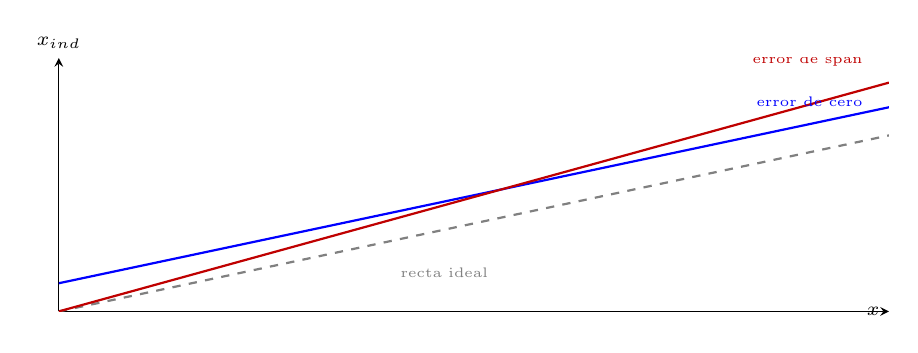
\begin{tikzpicture}
        \begin{axis}[
            width=\linewidth, height=4.8cm,
            xlabel={$x$}, ylabel={$x_{ind}$},
            xmin=0, xmax=5, ymin=0, ymax=7.2,
            axis lines=left, font=\scriptsize,
            xtick=\empty, ytick=\empty,
            every axis y label/.style={at=(current axis.above origin),anchor=south},
            every axis x label/.style={at=(current axis.right of origin),anchor=east},
        ]
            \addplot[gray, dashed, thick, domain=0:5] {x};
            \addplot[blue, thick, domain=0:5] {x+0.8};
            \addplot[red!75!black, thick, domain=0:5] {1.3*x};
            \node[gray, font=\tiny, anchor=north west] at (axis cs:2.0,1.5) {recta ideal};
            \node[blue, font=\tiny, anchor=south east] at (axis cs:4.9,5.55) {error de cero};
            \node[red!75!black, font=\tiny, anchor=south east] at (axis cs:4.9,6.7) {error de span};
        \end{axis}
    \end{tikzpicture}
    \caption[Error de cero y error de span sobre la recta de calibración.]{Los dos defectos de una recta de calibración lineal. El error de cero desplaza la recta entera el mismo valor absoluto --el error relativo es mayor en el fondo del rango--, mientras que el error de span cambia su pendiente y el error crece con la lectura.}\label{fig:errores_cero_span}
\end{marginfigure}

La distinción no es académica: la calibración de un instrumento consiste precisamente en medir esos dos parámetros y corregirlos, ajustando el cero y el span contra un patrón, y por eso el certificado de calibración de cualquier instrumento de laboratorio los declara por separado (Capítulo~\ref{cap:metrologia}). También explica por qué las especificaciones se escriben de dos formas a la vez: los errores de cero se dan en unidades absolutas --milivoltios, grados-- y los de span en tanto por ciento.

\marginnote{\textbf{Ejemplo:} un sensor con un error de span del \SI{0.5}{\percent} sobre un fondo de escala de \SI{100}{\milli\volt} y un error de cero de \SI{1}{\milli\volt}. En el fondo de escala el error combinado es de \SI{1.5}{\milli\volt}, es decir, el \SI{1.5}{\percent} de la lectura; pero a una décima parte del rango, con una lectura de \SI{10}{\milli\volt}, el error sigue siendo de \SI{1.05}{\milli\volt} y ahora representa el \SI{10.5}{\percent} de lo indicado. El error de cero manda en el fondo del rango y el de span, en el extremo superior.}

\subsection{Linealidad y Ajuste por Mínimos Cuadrados}

En ingeniería, siempre preferimos sistemas lineales de la forma $y = mx + b$, ya que facilitan el procesado posterior. Sin embargo, los sensores reales presentan desviaciones. Para obtener la \emph{mejor recta} de ajuste, que se considera la curva de calibración que representa a un sensor en el laboratorio, utilizamos el \emph{Método de los Mínimos Cuadrados}~\cite{taylor1997erroranalysis}, como se muestra en la Figura~\ref{fig:minimos_cuadrados}.
\begin{marginfigure}
    \centering
    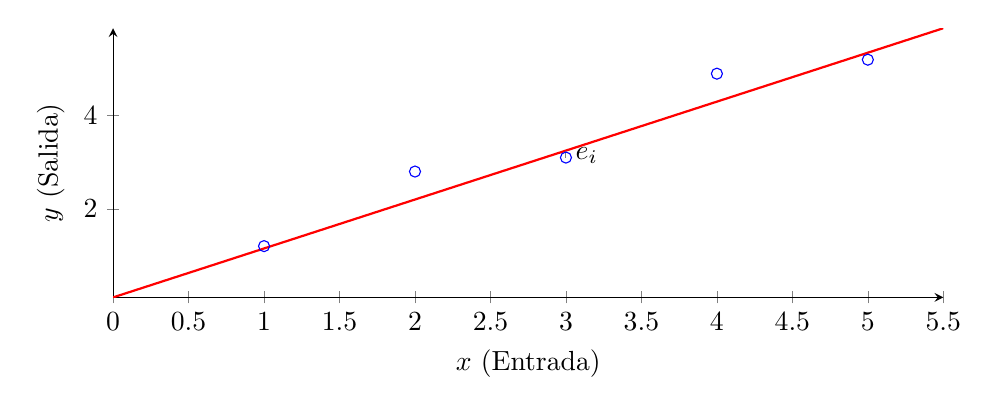
\begin{tikzpicture}
        \begin{axis}[
            width=\linewidth,
            height=5cm,
            xlabel={$x$ (Entrada)},
            ylabel={$y$ (Salida)},
            %font=\small,
            axis lines=left,
            scatter/classes={a={mark=o,draw=blue}},
            legend style={at={(0.5,-0.3)},anchor=north,legend columns=-1}
        ]
            % Puntos experimentales
            \addplot[scatter,only marks,scatter src=explicit symbolic]
                table[meta=label] {
                    x y label
                    1 1.2 a
                    2 2.8 a
                    3 3.1 a
                    4 4.9 a
                    5 5.2 a
                };
            % Recta de ajuste
            \addplot[thick, red, domain=0:5.5] {1.05*x + 0.1};
            
            % Línea de error (ejemplo)
            \draw[dashed, gray] (axis cs:3, 3.1) -- (axis cs:3, 3.25);
            \node[right] at (axis cs:3, 3.15) {$e_i$};
        \end{axis}
    \end{tikzpicture}
    \caption[Ajuste lineal por mínimos cuadrados.]{Ajuste lineal por mínimos cuadrados. La recta minimiza la distancia vertical al cuadrado de cada punto experimental.}\label{fig:minimos_cuadrados}
\end{marginfigure}

Dado un conjunto de $n$ pares de medidas $(x_i, y_i)$, buscamos la recta que minimiza la suma de los cuadrados de los residuos ($e_i$). El residuo para cada punto es la diferencia entre la salida medida $y_i$ y la salida predicha por la recta de ajuste $mx_i + b$:
\[ e_i = y_i - (mx_i + b) \]

El objetivo es encontrar los coeficientes $m$ y $b$ que minimizan la suma de los cuadrados de los residuos:
\begin{equation}\label{eq:error_cuadratico} 
    \sum_{i=1}^n e_i^2 = \sum_{i=1}^n {(y_i - (mx_i + b))}^2 = \sum_{i=1}^n {(y_i - mx_i - b)}^2
\end{equation}

Para obtener la mejor representación lineal de los datos obtenidos en el laboratorio, utilizamos el \emph{Método de los Mínimos Cuadrados}.\marginnote{\emph{Método de los Mínimos Cuadrados $m$ y $b$:}  La demostración de la Ecuación~\ref{eq:m_final} y~\ref{eq:b_final} se basa en la minimización de la función de error cuadrático proporcionada por la Ecuación~\ref{eq:error_cuadratico}, que es la suma de los cuadrados de los residuos. Al derivar esta función con respecto a $m$ y $b$ y establecer las derivadas iguales a cero, se obtienen las fórmulas mencionadas para $m$ y $b$. Este proceso asegura que se encuentra el punto mínimo de la función de error, lo que corresponde a la mejor recta de ajuste para los datos experimentales.

Para minimizar la función de error cuadrático $E(m, b) = \sum_{i=1}^n {(y_i - mx_i - b)}^2$, buscamos el punto donde las derivadas parciales se anulan:

\begin{enumerate}
    \item $\frac{\partial E}{\partial m} = -2\sum x_i (y_i - mx_i - b) = 0$
    \item $\frac{\partial E}{\partial b} = -2\sum (y_i - mx_i - b) = 0$
\end{enumerate}

Reorganizando términos (Ecuaciones Normales):
\begin{equation} \label{eq:normal1}
    m\sum x_i^2 + b\sum x_i = \sum x_i y_i
\end{equation}
\begin{equation} \label{eq:normal2}
    m\sum x_i + nb = \sum y_i
\end{equation}

Despejando $b$ de (\ref{eq:normal2}):
\[ b = \frac{\sum y_i - m\sum x_i}{n} = \bar{y} - m\bar{x} \]

Sustituyendo $b$ en (\ref{eq:normal1}) y resolviendo para $m$:
\begin{equation} \label{eq:m_final_note}
    m = \frac{n\sum x_i y_i - \sum x_i \sum y_i}{n\sum x_i^2 - {(\sum x_i)}^2}
\end{equation}

Estas expresiones permiten calcular la recta de mejor ajuste para cualquier conjunto de datos experimentales.
} Este método garantiza que la recta de ajuste $y = mx + b$ minimice la suma de los cuadrados de las distancias verticales (residuos) de cada punto experimental a la recta. Las fórmulas para calcular la pendiente ($m$) y la ordenada en el origen ($b$) son:

\begin{equation} \label{eq:m_final}
    m = \frac{n \sum\limits_{i=1}^n x_i y_i - \left(\sum\limits_{i=1}^n x_i\right) \left(\sum\limits_{i=1}^n y_i\right)}{n \sum\limits_{i=1}^n x_i^2 - {\left(\sum\limits_{i=1}^n x_i\right)}^2}
\end{equation}

\begin{equation} \label{eq:b_final}
    b = \bar{y} - m\bar{x} = \frac{\sum\limits_{i=1}^n y_i - m \sum\limits_{i=1}^n x_i}{n}
\end{equation}
donde $n$ es el número de pares de medidas $(x_i, y_i)$, y $\bar{x}, \bar{y}$ son las medias aritméticas de las muestras. 


En la Tabla~\ref{tab:datos_ejemplo} del siguiente ejemplo se muestra un conjunto de $n=5$ pares de medidas $(x_i, y_i)$ y la recta de ajuste encontrada por el Método de los Mínimos Cuadrados. La recta de ajuste es la que minimiza la suma de los cuadrados de los residuos.

\begin{margintable}
    \centering
    %\footnotesize
    \caption[Datos experimentales del sensor.]{Datos experimentales del sensor. Se muestra un conjunto de $n=5$ pares de medidas $(x_i, y_i)$ y la recta de ajuste encontrada por el Método de los Mínimos Cuadrados.\protect\label{tab:datos_ejemplo}}
    \begin{tabular}{c c}
        \toprule
        $x_i$ (bar) & $y_i$ (V) \\
        \midrule
        0 & 0.1 \\
        1 & 1.2 \\
        2 & 1.9 \\
        3 & 3.1 \\
        4 & 3.9 \\
        \bottomrule
    \end{tabular}
\end{margintable}

Para aplicar las fórmulas de mínimos cuadrados, calculamos primero las sumatorias necesarias:
\begin{itemize}
    \item $\sum x_i = 10$
    \item $\sum y_i = 10.2$
    \item $\sum x_i^2 = 0 + 1 + 4 + 9 + 16 = 30$
    \item $\sum x_i y_i = (0\cdot 0.1) + (1\cdot 1.2) + (2\cdot 1.9) + (3\cdot 3.1) + (4\cdot 3.9) = 29.9$
\end{itemize}

Sustituyendo en las expresiones de la pendiente ($m$) y la ordenada en el origen ($b$):
\begin{equation}
    m = \frac{5(29.9) - (10)(10.2)}{5(30) - (10)^2} = \frac{149.5 - 102}{150 - 100} = 0.95
\end{equation}
\begin{equation}
    b = \frac{10.2}{5} - 0.95\left(\frac{10}{5}\right) = 2.04 - 1.9 = 0.14
\end{equation}

La recta de ajuste resultante es \emph{$y = 0.95x + 0.14$} y está representada en la Figura~\ref{fig:grafico_ejemplo}.
\begin{marginfigure}
    \centering
    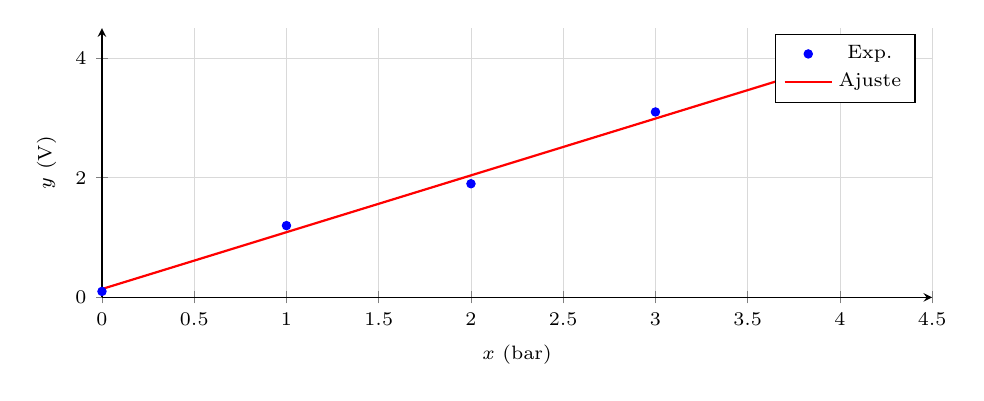
\begin{tikzpicture}
        \begin{axis}[
            width=\linewidth,
            height=5cm,
            xlabel={$x$ (bar)},
            ylabel={$y$ (V)},
            font=\scriptsize,
            grid=both,
            grid style={line width=.1pt, draw=gray!10},
            major grid style={line width=.2pt,draw=gray!30},
            axis lines=left,
            xmin=0, xmax=4.5,
            ymin=0, ymax=4.5
        ]
            % Puntos experimentales
            \addplot[
                only marks,
                mark=*,
                blue,
                mark size=1.5pt
            ] coordinates {
                (0, 0.1)
                (1, 1.2)
                (2, 1.9)
                (3, 3.1)
                (4, 3.9)
            };
            
            % Recta de ajuste: y = 0.95x + 0.14
            \addplot[
                thick,
                red,
                domain=0:4
            ] {0.95*x + 0.14};
            
            \legend{Exp., Ajuste}
        \end{axis}
    \end{tikzpicture}
    \caption[Representación de los puntos y la recta de ajuste calculada por el Método de los Mínimos Cuadrados.]{Representación de los puntos y la recta de ajuste calculada por el Método de los Mínimos Cuadrados.}\label{fig:grafico_ejemplo}
\end{marginfigure}

\subsection{Error de No Linealidad}\label{sec:error_no_linealidad}
Una vez calculados estos parámetros, el \emph{Error de No Linealidad}  se puede evaluar analizando el residuo máximo entre los valores medidos y los valores predichos por la recta de ajuste. El Error de No Linealidad se define como la máxima desviación de los puntos experimentales respecto a la recta de ajuste, expresado normalmente como porcentaje sobre el fondo de escala (\textit{Full Scale}, FS):

\begin{equation}
    \epsilon_{lin} = \frac{|y_i - (mx_i + b)|_{\max}}{y_{\max} - y_{\min}} \times 100\%
\end{equation}
para el ejemplo anterior, el error de no linealidad se calcularía evaluando el residuo máximo entre los valores medidos ($y_i$) y los valores predichos por la recta de ajuste ($mx_i + b$), y luego dividiendo por el rango total de salida ($y_{\max} - y_{\min}$) para obtener un porcentaje. Por lo tanto, el error de no linealidad se puede expresar como:

\begin{equation}
    \epsilon_{lin} = \frac{\max_i |y_i - (0.95x_i + 0.14)|}{3.9 - 0.1} \times 100\%
\end{equation}
donde $y_{\max} = 3.9$ V y $y_{\min} = 0.1$ V son los valores máximo y mínimo de la salida respectivamente. Este cálculo proporciona una medida cuantitativa de la desviación máxima de los puntos experimentales respecto a la recta de ajuste, lo que es crucial para evaluar la precisión del sensor en su rango de operación. Como $y_i$ valen 0.1, 1.2, 1.9, 3.1 y 3.9 V para $x_i$ igual a 0, 1, 2, 3 y 4 bar respectivamente, se evaluaría el residuo para cada punto y se identificaría el máximo para calcular el error de no linealidad. Así tenemos que el error de no linealidad se calcula evaluando el residuo para cada punto:
\begin{itemize}
    \item Para $x_0 = 0$ bar: $|0.1 - (0.95\cdot 0 + 0.14)| = |0.1 - 0.14| = 0.04$ V
    \item Para $x_1 = 1$ bar: $|1.2 - (0.95\cdot 1 + 0.14)| = |1.2 - 1.09| = 0.11$ V
    \item Para $x_2 = 2$ bar: $|1.9 - (0.95\cdot 2 + 0.14)| = |1.9 - 2.04| = 0.14$ V
    \item Para $x_3 = 3$ bar: $|3.1 - (0.95\cdot 3 + 0.14)| = |3.1 - 2.85| = 0.19$ V    
    \item Para $x_4 = 4$ bar: $|3.9 - (0.95\cdot 4 + 0.14)| = |3.9 - 3.64| = 0.21$ V
\end{itemize}
Por lo tanto, el residuo máximo es $0.21$ V para $x_4 = 4$ bar. Finalmente, el error de no linealidad se calcula como:
\begin{equation}
    \epsilon_{lin} = \frac{0.21}{3.9 - 0.1} \times 100\% \approx 5.38\%
\end{equation}
Esto indica que el error de no linealidad del sensor es aproximadamente del 5.38\% del fondo de escala, lo que proporciona una medida cuantitativa de la desviación máxima de los puntos experimentales respecto a la recta de ajuste, y es crucial para evaluar la precisión del sensor en su rango de operación. Un error de no linealidad del 5.38\% puede ser considerado aceptable o inaceptable dependiendo de los requisitos específicos de la aplicación para la cual se está utilizando el sensor. En aplicaciones donde se requiere alta precisión, este nivel de no linealidad podría ser problemático, mientras que en aplicaciones más tolerantes a la imprecisión, podría ser perfectamente adecuado. Por lo tanto, es importante evaluar este error en el contexto de la aplicación específica para determinar si el sensor cumple con los requisitos de precisión necesarios.




% \begin{itemize}
%     \item \emph{Error de No Linealidad}: Máxima desviación de los puntos experimentales respecto a la recta de ajuste, expresado normalmente como porcentaje sobre el fondo de escala (\textit{Full Scale}, FS).
%     \item \emph{Error de Histeresis}: Máxima diferencia en la salida para un mismo valor de entrada según el sentido de la variación (ascendente o descendente).
% \end{itemize}




\subsection{Recta de Referencia}
%que es la recta de referencia y como se define.

La recta de referencia, como se ilustra en la Figura~\ref{fig:recta_referencia}, es una linea que une el origen del sistema de coordenadas con el punto máximo de la salida. Esta recta se utiliza como una referencia para evaluar la linealidad y el comportamiento dinámico del sistema de medida. La elección de la recta de referencia es crucial, ya que puede influir en la interpretación de las características dinámicas del sensor, como la histéresis y la repetibilidad.

%ejemplo grafico de la recta de referencia y como se define.Dibujar una serie de puntos experimentales que no sean muy lineales y luego dibujar la recta de ajuste y la recta de referencia que los une. Explicar que esta recta se utiliza para evaluar la linealidad y el comportamiento dinámico del sistema de medida.
\begin{marginfigure}
    \centering
    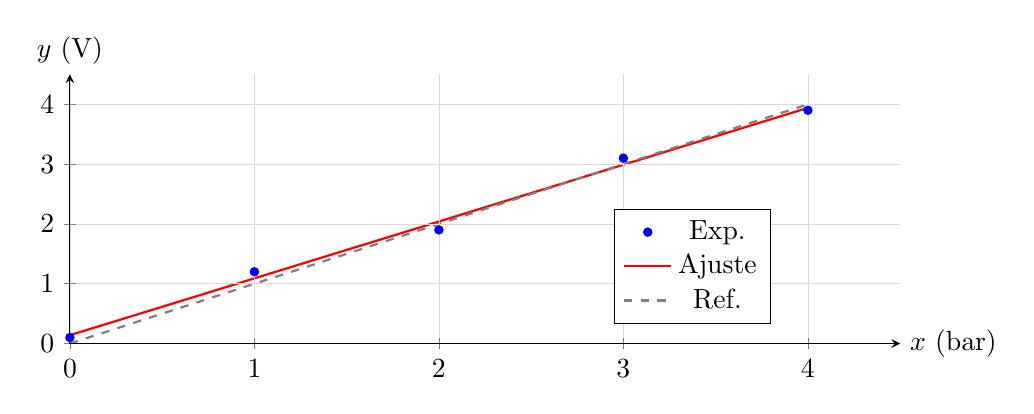
\begin{tikzpicture}
        \begin{axis}[
            width=\linewidth,
            height=5cm,
            xlabel={$x$ (bar)},
            ylabel={$y$ (V)},
            %font=\scriptsize,
            grid=both,
            grid style={line width=.1pt, draw=gray!10},
            major grid style={line width=.2pt,draw=gray!30},
            minor grid style={line width=.1pt,draw=gray!10},
            axis lines=left,
            every axis y label/.style={at=(current axis.above origin),anchor=south},
            every axis x label/.style={at=(current axis.right of origin),anchor=west},
            xmin=0, xmax=4.5,
            ymin=0, ymax=4.5,
            xtick={0,1,2,3,4},
            ytick={0,1,2,3,4},    
            xticklabels={$0$,$1$,$2$,$3$,$4$},
            yticklabels={$0$,$1$,$2$,$3$,$4$},
            enlargelimits=false, clip=false, axis on top,
            legend style={at={(0.75,0.5)}, anchor=north, legend columns=1},
        ]
            % Puntos experimentales
            \addplot[
                only marks,
                mark=*,
                blue,
                mark size=1.5pt
            ] coordinates {
                (0, 0.1)
                (1, 1.2)
                (2, 1.9)
                (3, 3.1)
                (4, 3.9)
            };
            
            % Recta de ajuste: y = 0.95x + 0.14
            \addplot[
                thick,
                red,
                domain=0:4
            ] {0.95*x + 0.14};
            
            % Recta de referencia: y = x
            \addplot[
                thick,
                dashed,
                gray,
                domain=0:4
            ] {x};
            \legend{Exp., Ajuste, Ref.}           
        \end{axis}       
    \end{tikzpicture}
    \caption[Recta de referencia y recta de ajuste]{
        Recta de referencia y recta de ajuste para una serie de puntos experimentales. 
    }\label{fig:recta_referencia}
\end{marginfigure}

% Como se define la recta de referencia. existen varias formas?
% la recta de referencia es una linea que une el origen del sistema de coordenadas con el punto máximo de la salida.

% Existen diferentes formas de definir la recta de referencia. La recta de referencia puede ser elegida basada en las siguientes características dinámicas:
% \begin{enumerate}
%     \item \emph{Linealidad de terminales}: Recta que une el origen y el punto máximo.
%     \item \emph{Linealidad a través de cero}: Obliga a que $b=0$.
%     \item \emph{Mejor recta de ajuste}: La obtenida por mínimos cuadrados (la más común).
% \end{enumerate}

\subsection{Histéresis y Repetibilidad}\label{sec:histeresis_repetibilidad}

Un sistema presenta \emph{histéresis} cuando la salida depende de la dirección en la que se alcanza la entrada (ascendente o descendente). Por ejemplo, si se aumenta la entrada $x$ desde un valor bajo hasta un valor alto, la salida $y$ puede seguir una curva diferente a la que se obtiene al disminuir $x$ desde el valor alto hasta el valor bajo. Esto se debe a que el sistema puede tener memoria o inercia, lo que provoca que la salida no solo dependa del valor actual de la entrada, sino también de su historia reciente. La histéresis es común en sensores magnéticos y mecánicos debido a la fricción o deformación elástica. En la Figura~\ref{fig:histeresis} se muestra un ejemplo gráfico del efecto de histéresis, donde la curva azul representa la variación ascendente de la entrada y la curva roja representa la variación descendente. La diferencia entre ambas curvas para el mismo rango de valores de entrada es una manifestación clara de la histéresis en el sistema.\marginnote{\textbf{Ejemplo de histéresis.} Un ejemplo típico de histéresis es el comportamiento de un motor de paso, donde la velocidad de rotación puede variar dependiendo de la dirección en la que se mueve el eje. Otro ejemplo típico de histéresis es el comportamiento de un termistor NTC\, donde la resistencia varía con la temperatura, pero la respuesta puede diferir dependiendo de si la temperatura está aumentando o disminuyendo, lo que es una manifestación de histéresis térmica.}

\begin{marginfigure}
    \centering
    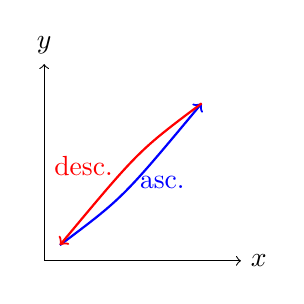
\begin{tikzpicture}
      \shorthandoff{>}
        \draw[->] (0,0) -- (2.5,0) node[right] {$x$};
        \draw[->] (0,0) -- (0,2.5) node[above] {$y$};
        % Curva ascendente
        \draw[blue, thick, ->] (0.2,0.2) .. controls (1,0.8) .. (2,2);
        % Curva descendente
        \draw[red, thick, ->] (2,2) .. controls (1.2,1.4) .. (0.2,0.2);
        \node[blue] at (1.5,1) {asc.};
        \node[red] at (.5,1.2) {desc.};
    \end{tikzpicture}
    \caption[Efecto de histéresis.]{Efecto de histéresis. Es común en sensores magnéticos y mecánicos debido a la fricción o deformación elástica.}\label{fig:histeresis}
\end{marginfigure}

%banda de Muerta

La \emph{banda muerta} es un fenómeno relacionado con la histéresis, donde existe un rango de valores de entrada que no produce ningún cambio en la salida. Esto es común en sistemas mecánicos con fricción o en sensores que requieren una fuerza mínima para activar la salida. Por ejemplo, en un reductor mecánico, puede haber una banda de muerta debido a la fricción interna, lo que significa que pequeñas variaciones en la entrada no se traducen en cambios en la salida hasta que se supera un umbral específico. En la Figura~\ref{fig:banda_muerta} se muestra un ejemplo gráfico de una banda de muerta, donde la curva azul representa la respuesta del sistema a variaciones de entrada. En el rango marcado como \emph{Banda de Muerta}, la salida permanece constante a pesar de las variaciones en la entrada, lo que ilustra claramente este fenómeno.\marginnote{\textbf{Ejemplo de Banda de Muerta.} Un ejemplo típico de banda de muerta es el comportamiento de un reductor mecánico, donde puede haber una banda de muerta debido a la fricción interna, lo que significa que pequeñas variaciones en la entrada no se traducen en cambios en la salida hasta que se supera un umbral específico. Otro ejemplo típico de banda de muerta es el comportamiento de un sensor de presión, donde puede haber una banda de muerta debido a la necesidad de superar una presión mínima para activar la salida del sensor.}

\begin{marginfigure}
    \centering
    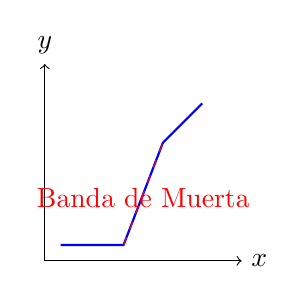
\begin{tikzpicture}
      \shorthandoff{>}
        \draw[->] (0,0) -- (2.5,0) node[right] {$x$};
        \draw[->] (0,0) -- (0,2.5) node[above] {$y$};
        % Curva con banda de muerta
        \draw[blue, thick] (0.2,0.2) -- (1,0.2) -- (1.5,1.5) -- (2,2);
        % Banda de muerta
        \draw[dashed, red] (1,0.2) -- (1.5,1.5);
        \node[red] at (1.25,0.8) {Banda de Muerta};
    \end{tikzpicture}
    \caption[Ejemplo de banda muerta.]{Ejemplo de banda muerta. Es común en sistemas mecánicos con fricción o en sensores que requieren una fuerza mínima para activar la salida.}\label{fig:banda_muerta}
\end{marginfigure}

La \emph{repetibilidad} es la capacidad de un sensor para entregar la misma salida al aplicar la misma entrada varias veces en periodos cortos de tiempo. Un sensor con buena repetibilidad producirá resultados consistentes bajo las mismas condiciones de prueba, lo que es crucial para aplicaciones donde se requiere alta precisión y confiabilidad. La repetibilidad se puede evaluar realizando múltiples mediciones con el mismo valor de entrada y analizando la variación en las salidas obtenidas. Un sensor con alta repetibilidad tendrá una desviación estándar baja en sus mediciones, lo que indica que las salidas son consistentes y confiables. En la Figura~\ref{fig:repetibilidad} se muestra un ejemplo gráfico de repetibilidad, donde se realizan varias mediciones con el mismo valor de entrada. La dispersión de los puntos alrededor de la media indica el nivel de repetibilidad del sensor, siendo una dispersión menor indicativa de una mejor repetibilidad.\marginnote{\textbf{Ejemplo de repetibilidad.} Un ejemplo típico de repetibilidad es el comportamiento de un sensor de temperatura, donde se espera que el sensor entregue la misma salida para la misma temperatura en múltiples mediciones realizadas en periodos cortos de tiempo. Otro ejemplo típico de repetibilidad es el comportamiento de un sensor de presión, donde se espera que el sensor entregue la misma salida para la misma presión en múltiples mediciones realizadas en periodos cortos de tiempo.} 

% \begin{margintable}
%     \centering
%     %\footnotesize
%     \begin{tabular}{c c}
%         \toprule
%         Medición (20 ºC) & Salida (V) \\
%         \midrule
%         1 & 2.0 \\
%         2 & 1.9 \\
%         3 & 2.1 \\
%         4 & 2.0 \\
%         5 & 1.95 \\
%         \bottomrule
%         \\
%     \end{tabular}
%     \caption{Ejemplo de repetibilidad. Se muestran varias mediciones con el mismo valor de entrada y la variación en las salidas obtenidas para evaluar la repetibilidad del sensor.}
%     \label{tab:repetibilidad}
% \end{margintable}

\begin{marginfigure}
    \centering
    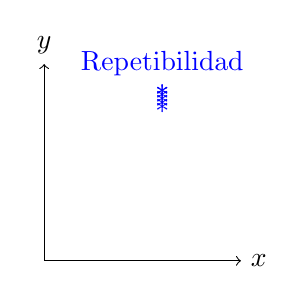
\begin{tikzpicture}
      \shorthandoff{>}
        \draw[->] (0,0) -- (2.5,0) node[right] {$x$};
        \draw[->] (0,0) -- (0,2.5) node[above] {$y$};
        % Puntos de repetibilidad dibujados con node como puntos azules 
        \node[blue] at (1.5,2.1) {*};
        \node[blue] at (1.5,2.0) {*};
        \node[blue] at (1.5,1.9) {*};
        \node[blue] at (1.5,2.1) {*};
        \node[blue] at (1.5,2.05) {*};
        \node[blue] at (1.5,1.95) {*};        
        \node[blue] at (1.5,2.5) {Repetibilidad};
    \end{tikzpicture}
    \caption[Ejemplo de repetibilidad.]{Ejemplo de repetibilidad. Un sensor con buena repetibilidad producirá resultados consistentes bajo las mismas condiciones de prueba.}\label{fig:repetibilidad}
\end{marginfigure}

\subsection{Error de Histéresis}


Además, el \emph{Error de Histeresis} se puede evaluar comparando las salidas para un mismo valor de entrada según el sentido de la variación (ascendente o descendente). Este error se define como la máxima diferencia en la salida para un mismo valor de entrada según el sentido de la variación, y se expresa también como porcentaje sobre el fondo de escala:

\begin{equation}    
    \epsilon_{his} = \frac{|y_{asc} - y_{desc}|_{\max}}{y_{\max} - y_{\min}} \times 100\%
\end{equation}
donde $y_{asc}$ y $y_{desc}$ son las salidas correspondientes a un mismo valor de entrada durante la variación ascendente y descendente respectivamente. Este cálculo proporciona una medida cuantitativa de la diferencia máxima en la salida para un mismo valor de entrada según el sentido de la variación, lo que es fundamental para evaluar la estabilidad y confiabilidad del sensor en aplicaciones donde se esperan cambios frecuentes en la magnitud medida.

\subsection{Rango de Entrada y Saturación}

Todo sistema de medida está diseñado para operar dentro de un intervalo específico de la magnitud de entrada $[x_{\min}, x_{\max}]$. El Fondo de Escala (Full Scale, FS) es la diferencia entre el valor máximo y el valor mínimo medible: $FS = x_{\max} - x_{\min}$. Define la capacidad total del instrumento.
    
La saturación es una característica no lineal que ocurre cuando la entrada excede los límites de diseño. En este estado, la salida $y$ deja de responder a incrementos de la entrada $x$, permaneciendo constante en un valor máximo ($y_{sat}$). En la Figura~\ref{fig:saturacion} se muestra un ejemplo gráfico de saturación, donde la curva azul representa la relación entre la entrada $x$ y la salida $y$. En la zona lineal (hasta $x_{sat}$), la salida aumenta proporcionalmente a la entrada. Sin embargo, una vez que se alcanza el punto de saturación ($x_{sat}$), la salida se mantiene constante en $y_{sat}$, independientemente de cualquier aumento adicional en la entrada. Esto ilustra claramente cómo la saturación limita el rango operativo del sistema de medida y afecta su capacidad para seguir cambios en la magnitud física más allá de ciertos límites.\marginnote{\textbf{Saturación:} Un sistema debe diseñarse para que su rango dinámico de trabajo nunca alcance la saturación, ya que en esa zona la sensibilidad es nula ($S = dy/dx = 0$) y la información de la magnitud física se pierde por completo.
}

\begin{marginfigure}
    \centering
    \shorthandoff{>}
    \begin{tikzpicture}
        \begin{axis}[
            width=\linewidth, height=4.5cm,
            xlabel={$x$}, ylabel={$y$},
            font=\scriptsize,
            axis lines=left,
            xmin=0, xmax=5, ymin=0, ymax=3.5,
            xtick={3}, xticklabels={$x_{sat}$},
            ytick={3}, yticklabels={$y_{sat}$},
            every axis y label/.style={at=(current axis.above origin),anchor=south},
            every axis x label/.style={at=(current axis.right of origin),anchor=west},
        ]
            % Zona lineal
            \addplot[thick, blue, domain=0:3] {x};
            % Zona de saturación
            \addplot[thick, red, domain=3:5] {3};
            % Línea discontinua ideal (prolongación)
            \addplot[dashed, gray, domain=3:4.5] {x};
            
            \node[blue, rotate=43] at (axis cs:1.2,1.6) {Zona Lineal};
            \node[red] at (axis cs:4,3.2) {Saturación};
        \end{axis}
    \end{tikzpicture}
    \caption[Característica de saturación.]{Característica de saturación. Físicamente, suele estar impuesta por los límites de alimentación de la electrónica o la deformación máxima del material del sensor.}\label{fig:saturacion}
\end{marginfigure}

\subsection{Efecto de Carga e Impedancias}\label{sub:efecto_carga_general}

Al conectar la salida de una etapa con la entrada de la siguiente --el sensor con el acondicionador, el acondicionador con el convertidor, el instrumento con el sistema de registro-- no se unen dos terminales ideales, sino una fuente con impedancia de salida $R_{out}$ y una carga con impedancia de entrada $R_{in}$. Ambas forman un divisor de tensión, y la señal que llega al receptor ya no es la que salió de la fuente:
\begin{equation}\label{eq:error_carga}
    v_{rx} = v_{tx}\,\frac{R_{in}}{R_{in} + R_{out}}, \qquad \frac{\Delta v}{v_{tx}} \approx -\frac{R_{out}}{R_{in}} \quad \text{si } R_{in} \gg R_{out}
\end{equation}
La regla de diseño es, por tanto, que la impedancia de entrada sea mucho mayor que la de salida: dos órdenes de magnitud de diferencia dejan un error del orden del \SI{1}{\percent}. La gravedad del efecto depende de la impedancia de la fuente, y por eso conviene conocerla antes de elegir la etapa siguiente: un sensor pasivo de \SI{1}{\kilo\ohm} no puede leerse con una entrada de \SI{1}{\kilo\ohm} --se pierde la mitad de la señal--, mientras que un termopar de unos pocos ohmios apenas acusa una entrada de \SI{10}{\kilo\ohm}. En los sensores resistivos este mismo efecto es el que obliga a las configuraciones de tres y cuatro hilos (Figura~\ref{fig:efecto_carga}) y en el acondicionamiento es la razón de ser de la etapa de entrada del amplificador de instrumentación (Sección~\ref{sec:inamp}).

\marginnote{\textbf{Efecto de carga en cifras:} una fuente de \SI{1}{\kilo\ohm} leída por una entrada de \SI{100}{\kilo\ohm} pierde el \SI{1}{\percent} de la señal; con una entrada de \SI{1}{\mega\ohm}, pierde el \SI{0.1}{\percent}. Como el error es sistemático y depende de una impedancia que a su vez cambia con la temperatura, no se corrige en el software: se combate con una etapa de entrada de alta impedancia, como un seguidor de tensión o un amplificador de instrumentación.}

\section{Características Dinámicas}\label{sec:caract_dinamicas} 

Las características dinámicas describen el comportamiento de un sistema de medida cuando la magnitud física varía con el tiempo. A diferencia de las características estáticas, que se centran en la relación entre entrada y salida en condiciones de equilibrio o variaciones lentas, las características dinámicas analizan cómo el sistema responde a cambios rápidos en la magnitud medida, incluyendo aspectos como la velocidad de respuesta, la estabilidad y la capacidad para seguir señales de alta frecuencia.

Las características dinámicas analizan la respuesta del sistema cuando la entrada $x(t)$ varía rápidamente. Matemáticamente, se modelan mediante una ecuación diferencial lineal de coeficientes constantes:

\begin{equation}
    a_n \frac{d^n y}{dt^n} + \cdots + a_1 \frac{dy}{dt} + a_0 y = b_m \frac{d^m x}{dt^m} + \cdots + b_0 x
\end{equation}

\subsection{Sistema de Orden 0}
Un sistema de orden 0 es un sensor ideal. La salida sigue a la entrada instantáneamente sin retardo ni error dinámico como se muestra en la Figura~\ref{fig:orden_0}. Su ecuación es:
\[ y(t) = K \cdot x(t) \]
donde $K$ es una constante de ganancia. La sensibilidad estática $K     = b_0/a_0$ es la sensibilidad estática.
%Figura de larespuesta escalon de un sistema de orden 0, que es una linea recta que sigue a la entrada sin retardo ni error dinamico.
\begin{marginfigure}
    \centering
    \begin{tikzpicture}
        \begin{axis}[ 
            width=\linewidth, height=4.5cm,
            xlabel={$t$}, ylabel={$y(t)$},
            font=\scriptsize,
            axis lines=left,
            ymin=0, ymax=1.5,
            every axis y label/.style={at=(current axis.above origin),anchor=south},
            every axis x label/.style={at=(current axis.right of origin),anchor=west},
            %xtick={1}, %xticklabels={$\tau$},
            ytick={1,1.01}, yticklabels={K}
        ]
           % ENTRADA (Escalón en t=0)
            \addplot[thick, red, dashed, domain=0:4] {1.01};
            %\addlegendentry{Entrada $x(t)$}

            % SALIDA (Orden 0: Sigue instantáneamente)
            % Usamos una línea sólida azul justo encima
            \addplot[thick, blue, domain=0:4] {1};
            %\addlegendentry{Salida $y(t)$}
        \end{axis}
    \end{tikzpicture}
    \caption[Respuesta al escalón de un sistema de orden 0.]{Respuesta al escalón de un sistema de orden 0. La salida sigue a la entrada instantáneamente sin retardo ni error dinámico.}\label{fig:orden_0}
\end{marginfigure}

\subsection{Sistema de Primer Orden}
Corresponde a sensores con almacenamiento de energía (ej.\ una capacidad térmica de un termómetro o condensador en un circuito). En este caso la salida $y(t)$ depende de la entrada $x(t)$ y de la constante de tiempo $\tau$. Matemáticamente, se modela mediante una ecuación diferencial lineal de primer orden. Su ecuación es:
\[ \tau \frac{dy(t)}{dt} + y(t) = K \cdot x(t) \]
donde $K$ es una constante de ganancia. La sensibilidad estática $K = b_0/a_0$ es la sensibilidad estática. En la Figura~\ref{fig:primer_orden} se muestra la respuesta al escalón de un sistema de primer orden. La respuesta al escalón de un sistema de primer orden es una curva exponencial que se aproxima a un valor final $K \cdot x(t)$ con una constante de tiempo $\tau$ que es un parámetro crucial que define la rapidez del sensor, ya que determina cuánto tiempo tarda la salida en responder a un cambio en la entrada. Un valor de $\tau$ más pequeño indica una respuesta más rápida, mientras que un valor de $\tau$ más grande indica una respuesta más lenta.\marginnote{\textbf{Constante de Tiempo ($\tau$):} Es el parámetro que define la rapidez del sensor. Representa el tiempo necesario para que la salida alcance el \qty{63.2}{\percent} de su valor final ante un escalón.
}

% Figura que muestra el escalon en rojo y en azul la respuesta al escalon de un sistema de primer orden, que es una curva exponencial que se aproxima a un valor final $K \cdot x(t)$ con una constante de tiempo $\tau$ que determina la rapidez de la respuesta. Las líneas punteadas indican el tiempo $\tau$ necesario para que la salida alcance el \SI{63.2}{\percent} de su valor final. La constante de tiempo $\tau$ es un parámetro crucial que define la rapidez del sensor, ya que determina cuánto tiempo tarda la salida en responder a un cambio en la entrada. Un valor de $\tau$ más pequeño indica una respuesta más rápida, mientras que un valor de $\tau$ más grande indica una respuesta más lenta.
\begin{marginfigure}
    \centering
    \begin{tikzpicture}
        \begin{axis}[
            width=\linewidth, height=4.5cm,
            xlabel={$t$}, ylabel={$y(t)$},
            %font=\scriptsize,
            %rango del eje y es 0 a 2
            ymin=0, ymax=1.5,
            axis lines=left,
            every axis y label/.style={at=(current axis.above origin),anchor=south},
            every axis x label/.style={at=(current axis.right of origin),anchor=west},
            xtick={1}, xticklabels={$\tau$},
            ytick={0.63, 1}, yticklabels={0.63K, K}
        ]
            % Dibujar la curva azul expomnencial de la respuesta al escalón
            \addplot[thick, blue, domain=0:4, samples=50] {1-exp(-x)};
            % Dibujar líneas punteadas para indicar el tiempo $\tau$ y el valor 0.63K
            % Líneas punteadas de la constante de tiempo
            \draw[dashed, gray] (axis cs:1,0) -- (axis cs:1,0.632);
            \draw[dashed, gray] (axis cs:0,0.632) -- (axis cs:1,0.632);
            \addplot[thick, red, dashed, domain=0:4] {1};
        \end{axis}
    \end{tikzpicture}
    \caption[Respuesta al escalón de un sistema de 1er orden.]{Respuesta al escalón de un sistema de 1er orden. La curva azul representa la salida $y(t)$ que se aproxima a su valor final $K \cdot x(t)$ de manera exponencial, y las líneas punteadas indican el tiempo $\tau$ necesario para que la salida alcance el \SI{63.2}{\percent} de su valor final. }\label{fig:primer_orden}
\end{marginfigure}

\subsection{Sistema de Segundo Orden}\label{sec:segundo_orden}
Corresponde a sensores con almacenamiento de energía y  con oscilaciones (ej.\ un sistema mecánico con masa, resorte y amortiguador, como el que se ilustra en la Figura~\ref{fig:masa_resorte}). Este sistema mecánico se rige por la segunda ley de Newton, resultando en la ecuación diferencial de segundo orden. 
\begin{equation}\label{eq:segundo_orden}
m \frac{d^2y(t)}{dt^2} + c \frac{dy(t)}{dt} + ky(t) = F(t)
\end{equation}
donde $m$ es la masa, $c$ es el coeficiente de amortiguamiento, $k$ es la constante del resorte y $F(t)$ es la fuerza externa aplicada. En esta ecuación, el término $m \frac{d^2y(t)}{dt^2}$ representa la inercia del sistema, el término $c \frac{dy(t)}{dt}$ representa la fuerza de amortiguamiento que se opone al movimiento, y el término $ky(t)$ representa la fuerza restauradora del resorte. La respuesta dinámica de este sistema puede presentar oscilaciones dependiendo de los valores de $m$, $c$ y $k$, lo que hace que su análisis sea más complejo en comparación con los sistemas de orden 0 y 1.
%
% Mostrar figura de un sistema mecánico con masa, resorte y amortiguador.
\begin{marginfigure}
    \centering
    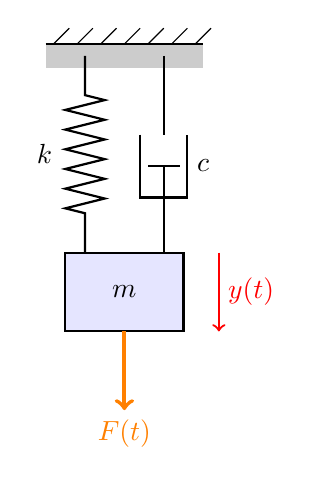
\begin{tikzpicture}[every node/.style={draw,outer sep=0pt,thick}]
        \shorthandoff{>}
        % Soporte superior (Techo)
        \node (ceiling) [shape=rectangle,fill=black!20,minimum width=2cm,minimum height=0.3cm,draw=none] at (0,0) {};
        \draw[thick] (-1,0.15) -- (1,0.15);
        \foreach \x in {-0.9,-0.6,...,0.9}
            \draw (\x,0.15) -- (\x+0.2,0.35);

        % Masa
        \node (M) [shape=rectangle,fill=blue!10,minimum width=1.5cm,minimum height=1cm] at (0,-3) {$m$};

        % Resorte (Spring) - Usando decoración zigzag
        \draw[decoration={zigzag,amplitude=2.5mm,segment length=2.5mm,post length=5mm,pre length=5mm},decorate,thick] 
            (-0.5,0) -- (-0.5,-2.5) node[midway,left=3mm,draw=none] {$k$};

        % Amortiguador (Damper) - Dibujo manual del pistón
        \begin{scope}[xshift=0.5cm]
            % Parte fija (cilindro)
            \draw[thick] (0,0) -- (0,-1);
            \draw[thick] (-0.3,-1) -- (-0.3,-1.8) -- (0.3,-1.8) -- (0.3,-1);
            % Parte móvil (pistón)
            \draw[thick] (0,-2.5) -- (0,-1.4);
            \draw[thick] (-0.2,-1.4) -- (0.2,-1.4);
            \node[draw=none] at (0.5,-1.4) {$c$};
        \end{scope}

        % Coordenada de desplazamiento
        \draw[->,thick,red] (1.2,-2.5) -- (1.2,-3.5) node[midway,right,draw=none] {$y(t)$};
        
        % Fuerza externa (opcional)
        \draw[->,line width=1.5pt,orange] (0,-3.5) -- (0,-4.5) node[below,draw=none] {$F(t)$};

    \end{tikzpicture}
    \caption[Sistema mecánico de segundo orden.]{Sistema mecánico de segundo orden. Los parámetros $m$ (masa), $k$ (constante elástica) y $c$ (coeficiente de amortiguamiento) definen la respuesta dinámica del sensor.}\label{fig:masa_resorte}
\end{marginfigure}
%
Comparando la expresión~\eqref{eq:segundo_orden} con la forma normalizada de un sistema de segundo orden:
\begin{equation}    
\frac{d^2 y(t)}{dt^2} + 2\zeta \omega_n \frac{dy(t)}{dt} + \omega_n^2 y(t) = \frac{F(t)}{m}
\end{equation}
podemos obtener las relaciones fundamentales para el diseño de sensores de segundo orden:
\begin{equation}
\omega_n = \sqrt{\frac{k}{m}} \quad  \quad \zeta = \frac{c}{2\sqrt{km}} \quad \quad K = \frac{1}{m\omega_n^2} = \frac{1}{k}
\end{equation}
donde $\omega_n$ es la \emph{frecuencia natural} del sistema, $\zeta$ es el \emph{factor de amortiguamiento} y $K$ es la sensibilidad estática.  

La frecuencia natural $\omega_n$ influye en la rapidez de la respuesta, siendo una frecuencia más alta indicativa de una respuesta más rápida. Esta respuesta al escalón de un sistema de segundo orden puede presentar oscilaciones dependiendo del valor del factor de amortiguamiento $\zeta$.%\marginnote{\textbf{Factor de Amortiguamiento ($\zeta$):} Es un parámetro que determina el tipo de respuesta del sistema. Si $\zeta < 1$, el sistema es subamortiguado y presenta oscilaciones. Si $\zeta = 1$, el sistema es críticamente amortiguado y alcanza su valor final sin oscilar. Si $\zeta > 1$, el sistema es sobreamortiguado y se aproxima a su valor final de manera exponencial sin oscilar.}
\begin{enumerate}
    \item Si $\zeta < 1$, el sistema es subamortiguado y la salida oscila antes de estabilizarse en su valor final.
    \item Si $\zeta = 1$, el sistema es críticamente amortiguado y la salida alcanza su valor final sin oscilar.
    \item Si $\zeta > 1$, el sistema es sobreamortiguado y la salida se aproxima a su valor final de manera exponencial.
\end{enumerate}
%\marginnote{\textbf{Frecuencia Natural ($\omega_n$):} Es un parámetro que influye en la rapidez de la respuesta del sistema. Una frecuencia natural más alta indica una respuesta más rápida, mientras que una frecuencia natural más baja indica una respuesta más lenta.}

 %

%
En la Figura~\ref{fig:segundo_orden} se muestra la respuesta al escalón de un sistema de segundo orden. En el caso de un sistema de segundo orden \emph{subamortiguado}, la ecuación que gobierna la respuesta al escalón es:
\begin{equation}
    y(t) = K \left( 1 - e^{-\zeta \omega_n t} \left( \cos(\omega_d t) + \frac{\zeta}{\sqrt{1-\zeta^2}} \sin(\omega_d t) \right) \right)
\end{equation}
donde $\omega_d = \omega_n \sqrt{1-\zeta^2}$ es la frecuencia de oscilación amortiguada. En esta ecuación, el término $e^{-\zeta \omega_n t}$ representa la envolvente de decaimiento de las oscilaciones, mientras que la combinación de las funciones trigonométricas describe la naturaleza oscilatoria del sistema. La sobreoscilación máxima $M_p$ se puede calcular como:
\begin{equation}
    M_p = e^{-\frac{\pi \zeta}{\sqrt{1-\zeta^2}}}
\end{equation}
que representa la máxima desviación de la salida respecto al valor final durante las oscilaciones. La frecuencia de oscilación amortiguada $\omega_d$ también influye en la rapidez de las oscilaciones, siendo una frecuencia más alta indicativa de oscilaciones más rápidas. En resumen, la respuesta al escalón de un sistema de segundo orden subamortiguado se caracteriza por una combinación de un crecimiento exponencial amortiguado y oscilaciones sinusoidales, donde la magnitud de la sobreoscilación y la frecuencia de las oscilaciones dependen del factor de amortiguamiento $\zeta$ y la frecuencia natural $\omega_n$ del sistema.
% Figura que muestra el escalon en rojo y en azul la respuesta al escalon de un sistema de segundo orden, que puede presentar oscilaciones dependiendo del valor del factor de amortiguamiento $\zeta$. Si $\zeta < 1$, el sistema es subamortiguado y la salida oscila antes de estabilizarse en su valor final. Si $\zeta = 1$, el sistema es críticamente amortiguado y la salida alcanza su valor final sin oscilar. Si $\zeta > 1$, el sistema es sobreamortiguado y la salida se aproxima a su valor final de manera exponencial sin oscilar. La frecuencia natural $\omega_n$ también influye en la rapidez de la respuesta, siendo una frecuencia más alta indicativa de una respuesta más rápida.
\begin{marginfigure}
    \centering
    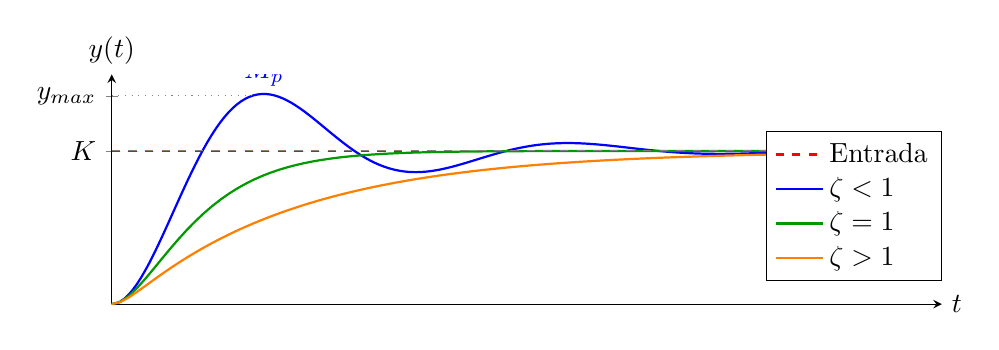
\begin{tikzpicture}
        \begin{axis}[
            width=\linewidth, height=4.5cm,
            xlabel={$t$}, ylabel={$y(t)$},
            %font=\scriptsize,
            ymin=0, ymax=1.5, xmin=0, xmax=6,
            axis lines=left,
            % IMPORTANTE: Usar radianes para las funciones trigonométricas
            trig format plots=rad, 
            every axis y label/.style={at=(current axis.above origin),anchor=south},
            every axis x label/.style={at=(current axis.right of origin),anchor=west},
            % Etiquetas correctas para 2º orden
            xtick=\empty,
            ytick={1, 1.36}, yticklabels={$K$, $y_{max}$},
            legend style={at={(1,0.1)}, anchor=south east, cells={anchor=west}}
        ]
            % 1. ESCALÓN DE ENTRADA
            \addplot[thick, red, dashed, domain=0:6] {1};
            \addlegendentry{Entrada}

            % 2. SUBAMORTIGUADO (zeta = 0.3, wn = 3) - CORRECTO
            \addplot[thick, blue, domain=0:6, samples=200] 
                {1 - exp(-0.9*x) * (cos(2.86*x) + 0.314*sin(2.86*x))};
            \addlegendentry{$\zeta < 1$}
            
            % Marcador de Sobreoscilación para el azul
            \draw[dotted, gray] (axis cs:0,1.36) -- (axis cs:1.1,1.36);
            \node[anchor=south, blue] at (axis cs:1.1, 1.36) {$M_p$};

            % 3. CRÍTICAMENTE AMORTIGUADO (zeta = 1, wn = 3)
            % Fórmula: y(t) = 1 - (1 + wn*t)*exp(-wn*t)
            \addplot[thick, green!60!black, domain=0:6, samples=100] 
                {1 - (1 + 3*x)*exp(-3*x)};
            \addlegendentry{$\zeta = 1$}
            
            % 4. SOBREAMORTIGUADO (zeta = 2, wn = 3)
            % Fórmula: suma de dos exponenciales reales
            \addplot[thick, orange, domain=0:6, samples=100] 
                {1 - 1.077*exp(-0.804*x) + 0.077*exp(-11.19*x)};
            \addlegendentry{$\zeta > 1$}

            % Línea de valor final
            \draw[dashed, gray] (axis cs:0,1) -- (axis cs:6,1);
        \end{axis}
    \end{tikzpicture}
    \caption[Respuesta al escalón de un sistema de segundo orden.]{Respuesta al escalón de un sistema de segundo orden. Las curvas representan las salidas $y(t)$ que puedes presentar oscilaciones dependiendo del valor del factor de amortiguamiento $\zeta$. En este caso, se muestra un sistema subamortiguado ($\zeta < 1$) donde la salida oscila antes de estabilizarse en su valor final; un sistema críticamente amortiguado ($\zeta = 1$) donde la salida alcanza su valor final sin oscilar; y un sistema sobreamortiguado ($\zeta > 1$) donde la salida se aproxima a su valor final de manera exponencial sin oscilar.}\label{fig:segundo_orden}
\end{marginfigure}


En el caso de un sistema de segundo orden \emph{críticamente amortiguado}, la ecuación que gobierna la respuesta al escalón es:
\begin{equation}
    y(t) = K \left( 1 - (1 + \omega_n t) e^{-\omega_n t} \right)
\end{equation}
donde $\omega_n$ es la frecuencia natural del sistema. En esta ecuación, el término $(1 + \omega_n t) e^{-\omega_n t}$ representa la combinación de un crecimiento lineal y un decaimiento exponencial que caracteriza la respuesta de un sistema críticamente amortiguado. La salida $y(t)$ se aproxima a su valor final $K$ sin presentar oscilaciones, y la rapidez con la que alcanza el valor final está determinada por la frecuencia natural $\omega_n$. En resumen, la respuesta al escalón de un sistema de segundo orden críticamente amortiguado se caracteriza por una aproximación suave al valor final sin oscilaciones, donde la rapidez de la respuesta está influenciada por la frecuencia natural del sistema.    

Y por último, en el caso de un sistema de segundo orden \emph{sobreamortiguado}, las raíces de la ecuación característica son reales y distintas. La respuesta al escalón no presenta oscilaciones y es más lenta que en el caso crítico, la ecuación que gobierna la respuesta al escalón es:
\begin{equation}
y(t) = K \left( 1 - \frac{s_2}{s_2 - s_1} e^{s_1 t} + \frac{s_1}{s_2 - s_1} e^{s_2 t} \right)
\end{equation}
donde $s_1$ y $s_2$ son las raíces reales de la ecuación característica dada por:
\begin{equation}
s_{1,2} = -\zeta \omega_n \pm \omega_n \sqrt{\zeta^2 - 1}
\end{equation}
En esta ecuación, el término $\frac{s_2}{s_2 - s_1} e^{s_1 t}$ y $\frac{s_1}{s_2 - s_1} e^{s_2 t}$ representan la combinación de dos exponenciales reales que caracterizan la respuesta de un sistema sobreamortiguado. La salida $y(t)$ se aproxima a su valor final $K$ de manera más lenta que en el caso críticamente amortiguado, y no presenta oscilaciones. La rapidez con la que alcanza el valor final está determinada por las raíces $s_1$ y $s_2$, que a su vez dependen del factor de amortiguamiento $\zeta$ y la frecuencia natural $\omega_n$ del sistema.\marginnote{\textbf{Raíces Reales:} En un sistema de segundo orden sobreamortiguado, las raíces de la ecuación característica son reales y negativas, lo que garantiza que los términos exponenciales decaigan hacia cero, permitiendo que la salida alcance el valor final $K$ de manera lenta que en el caso críticamente amortiguado. Las raíces reales son determinadas por el factor de amortiguamiento $\zeta$ y la frecuencia natural $\omega_n$ del sistema.}

\subsection{Ejemplo de Cálculo de la Respuesta al Escalón de un Sistema de Segundo Orden con $\zeta = 0.3$ y $\omega_n = 3$}\label{sec:ejemplo_segundo_orden}

A modo de ejemplo, en la Figura~\ref{fig:ejemplo_segundo_orden} se muestra el cálculo de la respuesta al escalón de un sistema de segundo orden con $\zeta = 0.3$ y $\omega_n = 3$. El sistema es subamortiguado ($\zeta < 1$) y la salida oscila antes de estabilizarse en su valor final. La curva azul representa la salida $y(t)$ que se aproxima a su valor final $K$ de manera exponencial amortiguada y oscilatoria, donde la magnitud de la sobreoscilación $M_p$ y la frecuencia de las oscilaciones dependen del factor de amortiguamiento $\zeta=0.3$ y la frecuencia natural $\omega_n=3$ del sistema. En este caso, se observa que la salida oscila antes de estabilizarse en su valor final, lo que es característico de un sistema subamortiguado. 

La magnitud de la sobreoscilación $M_p$ se calcula de la siguiente forma:
\begin{equation}
    M_p = e^{-\frac{\pi \zeta}{\sqrt{1-\zeta^2}}} = e^{-\frac{\pi \cdot 0.3}{\sqrt{1-0.3^2}}} \approx 0.372
\end{equation}
lo que indica que la salida alcanza un máximo de aproximadamente $1.37K$ antes de estabilizarse en su valor final $K$. La frecuencia de las oscilaciones amortiguadas $\omega_d$ se calcula como:
\begin{equation}
    \omega_d = \omega_n \sqrt{1-\zeta^2} = 3 \sqrt{1-0.3^2} \approx \SI{2.86}{rad/s}
\end{equation}
A partir de este valor, podemos predecir el instante en el que ocurrirá el primer pico (tiempo de pico, $t_p$):
\begin{equation}
    t_p = \frac{\pi}{\omega_d} = \frac{\pi}{2.86} \approx \SI{1.1}{s}
\end{equation}
La caracterización dinámica obtenida para el sistema ($\zeta = 0.3$ y $\omega_n = \SI{3}{rad/s}$) permite extraer conclusiones críticas sobre la calidad de la medida en régimen transitorio:

\begin{itemize}
    \item \emph{Frecuencia Amortiguada ($\omega_d$)}: El valor de $\omega_d \approx \SI{2.86}{rad/s}$ determina la \textit{periodicidad del transitorio}. Físicamente, representa la velocidad a la que el sistema oscila antes de alcanzar el equilibrio. Una $\omega_d$ más elevada es un indicador directo de una \emph{respuesta más rápida}, reduciendo el tiempo necesario para que el sensor reaccione inicialmente, aunque puede comprometer la estabilidad si el amortiguamiento es bajo.
    
    \item \emph{Sobreoscilación Máxima ($M_p$)}: El resultado de \SI{37.2}{\percent} indica que el sensor experimentará un \textit{error dinámico temporal} considerable, superando el valor real de la magnitud física en más de un tercio de su valor de estado estacionario ($K$). 
    
    \item \emph{Tiempo de Pico ($t_p$)}: Este error máximo ocurre exactamente a los \SI{1.1}{s} tras la aparición del escalón. Para un ingeniero de instrumentación, este dato es vital: cualquier captura de datos (muestreo) realizada cerca de este instante daría una lectura errónea y sobredimensionada de la magnitud real.
\end{itemize}
\marginnote{\textbf{Compromiso de Diseño:} En instrumentación, existe un \textit{trade-off} constante. Aumentar la rapidez (subir $\omega_n$) suele desplazar el tiempo de pico $t_p$ hacia la izquierda (más rápido), pero si no se controla el factor de amortiguamiento $\zeta$, la sobreoscilación $M_p$ puede dañar el sistema o saturar las etapas de amplificación posteriores.}

En resumen, el sistema analizado es capaz de seguir cambios con una rapidez moderada ($\omega_d \approx \SI{2.86}{rad/s}$), pero a costa de un transitorio oscilatorio pronunciado que requiere esperar al menos hasta el \emph{tiempo de establecimiento} ($t_s$) para que la medida se considere válida y dentro de una banda de error aceptable.

%ejemplo de calculo de la respuesta al escalon de un sistema de segundo orden subamortiguado, con $\zeta = 0.3$ y $\omega_n = 3$.
\begin{marginfigure}
    \centering
    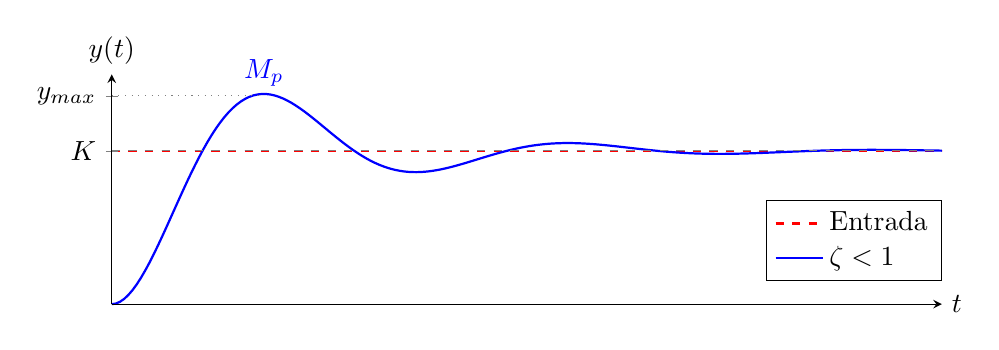
\begin{tikzpicture}
        \begin{axis}[
            width=\linewidth, height=4.5cm,
            xlabel={$t$}, ylabel={$y(t)$},
            %font=\scriptsize,
            ymin=0, ymax=1.5, xmin=0, xmax=6,            
            axis lines=left,            
            % IMPORTANTE: Usar radianes para las funciones trigonométricas
            trig format plots=rad,            
            every axis y label/.style={at=(current axis.above origin),anchor=south},            
            every axis x label/.style={at=(current axis.right of origin),anchor=west},            
            enlargelimits=false, clip=false, axis on top,
            legend style={at={(1,0.1)}, anchor=south east, cells={anchor=west}},
            % Etiquetas correctas para 2º orden
            xtick=\empty,
            ytick={1, 1.36}, yticklabels={$K$, $y_{max}$},
        ]
            % 1. ESCALÓN DE ENTRADA
            \addplot[thick, red, dashed, domain=0:6] {1};
            \addlegendentry{Entrada}

            % 2. SUBAMORTIGUADO (zeta = 0.3, wn = 3) - CORRECTO
            \addplot[thick, blue, domain=0:6, samples=200] 
                {1 - exp(-0.9*x) * (cos(2.86*x) + 0.314*sin(2.86*x))};
            \addlegendentry{$\zeta < 1$}
            
            % Marcador de Sobreoscilación para el azul
            \draw[dotted, gray] (axis cs:0,1.36) -- (axis cs:1.1,1.36);
            \node[anchor=south, blue] at (axis cs:1.1, 1.36) {$M_p$};

            % Línea de valor final
            \draw[dashed, gray] (axis cs:0,1) -- (axis cs:6,1);
        \end{axis}
    \end{tikzpicture}
    \caption[Respuesta al escalón de un sistema de segundo orden.]{Ejemplo de cálculo de la respuesta al escalón de un sistema de segundo orden subamortiguado, con $\zeta = 0.3$ y $\omega_n = 3$. La curva azul representa la salida $y(t)$ que se aproxima a su valor final $K$ de manera exponencial amortiguada y oscilatoria, donde la magnitud de la sobreoscilación $M_p$ y la frecuencia de las oscilaciones dependen del factor de amortiguamiento $\zeta$ y la frecuencia natural $\omega_n$ del sistema.}\label{fig:ejemplo_segundo_orden}
\end{marginfigure}

\subsection{Prestaciones Dinámicas Normalizadas}\label{sub:prestaciones_dinamicas}

Los parámetros de las secciones anteriores --la constante de tiempo $\tau$, la frecuencia natural $\omega_n$ y el amortiguamiento $\zeta$-- describen el sistema, pero las hojas de características de los instrumentos y los pliegos de los ensayos no se escriben con ellos, sino con cifras medidas sobre la respuesta al escalón, que es lo que resume la Figura~\ref{fig:prestaciones_dinamicas}:

\begin{itemize}
    \item \emph{Tiempo de subida} ($t_r$): lo que tarda la salida en pasar del \SI{10}{\percent} al \SI{90}{\percent} de su valor final. Para un sistema de segundo orden vale aproximadamente $t_r \approx 1{,}8/\omega_n$: la frecuencia natural fija la rapidez.
    \item \emph{Sobreoscilación máxima} ($M_p$): el exceso sobre el valor final en el primer pico, en porcentaje. Depende solo del amortiguamiento,
\begin{equation}\label{eq:sobreoscilacion}
    M_p = e^{-\pi\zeta/\sqrt{1-\zeta^2}}
\end{equation}
y cae deprisa: un \SI{30.9}{\percent} para $\zeta = 0{,}35$, un \SI{16.3}{\percent} para $\zeta = 0{,}5$ y ninguna sobreoscilación para $\zeta \ge 1$.
    \item \emph{Tiempo de establecimiento} ($t_s$): lo que tarda la salida en quedarse dentro de una banda alrededor del valor final, del \SI{5}{\percent} o del \SI{2}{\percent} según lo que exija la especificación. Vale aproximadamente $t_s \approx 3/(\zeta\omega_n)$ al \SI{5}{\percent} y $t_s \approx 4/(\zeta\omega_n)$ al \SI{2}{\percent}: el amortiguamiento manda en la duración y la frecuencia natural, en la velocidad.
    \item \emph{Ancho de banda} ($f_c$): la frecuencia a la que la ganancia cae un factor $\sqrt{2}$ respecto a la de continua. Para $\zeta$ en torno a $0{,}7$ coincide, con buena aproximación, con la frecuencia natural.
\end{itemize}

\begin{marginfigure}
    \centering
    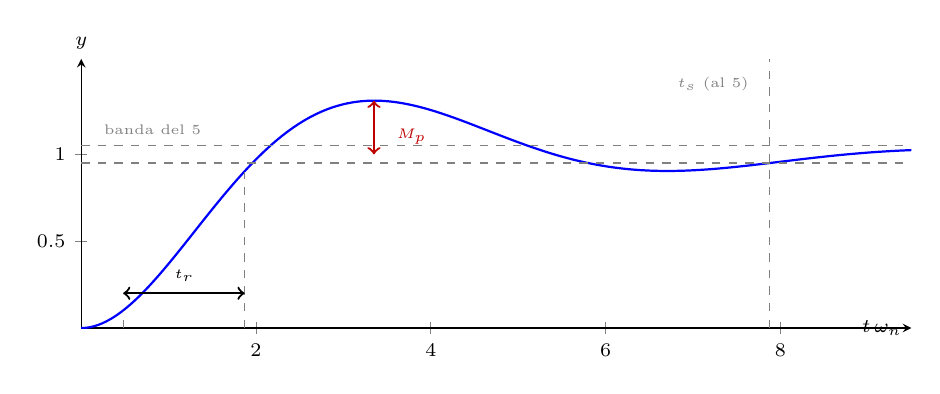
\begin{tikzpicture}
        \begin{axis}[
            width=\linewidth, height=5cm,
            xlabel={$t\,\omega_n$}, ylabel={$y$},
            xmin=0, xmax=9.5, ymin=0, ymax=1.55,
            axis lines=left, font=\scriptsize,
            xtick={2,4,6,8}, ytick={0.5,1},
            every axis y label/.style={at=(current axis.above origin),anchor=south},
            every axis x label/.style={at=(current axis.right of origin),anchor=east},
        ]
            \addplot[blue, thick, domain=0:9.5, samples=250]
                {1 - exp(-0.35*x)*(cos(deg(0.937*x)) + 0.374*sin(deg(0.937*x)))};
            % banda del 5 %
            \draw[dashed, gray] (axis cs:0,0.95) -- (axis cs:9.5,0.95);
            \draw[dashed, gray] (axis cs:0,1.05) -- (axis cs:9.5,1.05);
            \node[gray, font=\tiny, anchor=south west] at (axis cs:0.15,1.06) {banda del \SI{5}{\percent}};
            % sobreoscilación máxima
            \draw[<->, red!75!black, thick] (axis cs:3.35,1) -- (axis cs:3.35,1.309);
            \node[red!75!black, font=\tiny, anchor=west] at (axis cs:3.5,1.1) {$M_p$};
            % tiempo de subida (10 % a 90 %)
            \draw[dashed, gray] (axis cs:0.48,0) -- (axis cs:0.48,0.10);
            \draw[dashed, gray] (axis cs:1.87,0) -- (axis cs:1.87,0.90);
            \draw[<->, thick] (axis cs:0.48,0.2) -- (axis cs:1.87,0.2);
            \node[font=\tiny, anchor=south] at (axis cs:1.18,0.21) {$t_r$};
            % tiempo de establecimiento al 5 %
            \draw[dashed, gray] (axis cs:7.88,0) -- (axis cs:7.88,1.55);
            \node[gray, font=\tiny, anchor=north east] at (axis cs:7.75,1.5) {$t_s$ (al \SI{5}{\percent})};
        \end{axis}
    \end{tikzpicture}
    \caption[Prestaciones dinámicas medidas sobre la respuesta al escalón.]{Las prestaciones dinámicas que se especifican en una hoja de características, medidas sobre la respuesta al escalón de un sistema de segundo orden con $\zeta = 0{,}35$: el tiempo de subida $t_r$ (del \SI{10}{\percent} al \SI{90}{\percent}), la sobreoscilación máxima $M_p$ y el tiempo de establecimiento $t_s$ hasta entrar en la banda del \SI{5}{\percent}. El tiempo de subida y el de establecimiento fijan la rapidez; la sobreoscilación, el amortiguamiento.}\label{fig:prestaciones_dinamicas}
\end{marginfigure}

De los cuatro parámetros hay uno que merece una recomendación, porque aparece en todas las especificaciones y casi nunca se explica por qué: el amortiguamiento en torno a $\zeta \approx 0{,}7$ es el compromiso clásico, ya que da la respuesta más rápida sin sobreoscilación apreciable --menos de un \SI{5}{\percent}-- y un ancho de banda bien definido, con $f_c \approx \omega_n$. Es el valor que se busca cuando el ingeniero puede elegirlo --el amortiguamiento de un galvanómetro, la constante de tiempo de un filtro, el lazo de un circuito de disparo-- y el que conviene identificar en las especificaciones cuando viene impuesto.

\section{Límites de la Medida: Ruido y Rango Dinámico}\label{sec:limites_medida}

En esta sección se analizan los límites fundamentales de la medida, centrándonos en el ruido y el rango dinámico. Estos conceptos son cruciales para entender las limitaciones inherentes a cualquier sistema de medida y para diseñar sensores que puedan operar de manera efectiva dentro de estas limitaciones.

\subsection{El suelo de Ruido (\textit{Noise Floor})}\label{sec:noise_floor}
Una vez definidos los límites superiores (saturación), falta el límite inferior de la medida, que no es cero sino el \emph{suelo de ruido}: el nivel mínimo de señal que el sistema puede detectar por encima de su propio ruido --térmico, de disparo, de \textit{flicker}...--~\cite{ott1988noise}. Se expresa en las unidades de la magnitud medida, o en decibelios cuando conviene comparar rangos amplios. Su componente más predecible, el ruido térmico, se calcula como:
\begin{equation}\label{eq:noise_floor}
    N_f = \sqrt{4 k T R \Delta f}
\end{equation}
donde $k$ es la constante de Boltzmann, $T$ la temperatura absoluta, $R$ la resistencia del sistema y $\Delta f$ su ancho de banda: cuanto mayor sea cualquiera de los tres, mayor el ruido y peor la capacidad del sensor para detectar señales débiles.

\subsection{Ejemplo de Cálculo del Suelo de Ruido}\label{sec:ejemplo_suelo_ruido}
Con $R = \SI{1}{\kilo\ohm}$, $T = \SI{300}{\kelvin}$ y $\Delta f = \SI{1}{\kilo\hertz}$, la expresión~\eqref{eq:noise_floor} da:
\begin{equation}\label{eq:ejemplo_suelo_ruido}
    N_f = \sqrt{4 \cdot 1.38 \times 10^{-23} \cdot 300 \cdot 1000 \cdot 1000} \approx \SI{1.14}{\micro\volt}
\end{equation}
Ninguna señal por debajo de \SI{1.14}{\micro\volt} es fiable en este sistema. Bajar el suelo de ruido --componentes de bajo ruido, menor ancho de banda, un diseño de circuito cuidadoso-- es la única forma de detectar señales más débiles.

\subsection{Rango Dinámico}\label{sec:rango_dinamico}
El rango dinámico es la relación, en decibelios, entre la señal más fuerte que el sistema puede medir sin saturarse y la más débil que puede detectar por encima del suelo de ruido:
\begin{equation}\label{eq:rango_dinamico}
    R_D = 20 \log_{10} \left( \frac{S_{\max}}{N_f} \right)
\end{equation}
donde $S_{\max}$ es la señal máxima sin saturación y $N_f$ el suelo de ruido. Es una propiedad fija del sistema --no de la señal que se esté midiendo en cada momento-- y define su capacidad para medir simultáneamente señales muy grandes y muy pequeñas.\marginnote{\textbf{Importancia del Rango Dinámico:} Un micrófono con rango dinámico amplio captura tanto un susurro como un grito sin distorsión ni pérdida de información; de ahí que el rango dinámico se exprese en decibelios, que comprimen esas diferencias de varios órdenes de magnitud a una escala manejable.}

\subsection{Ejemplo de Cálculo del Rango Dinámico}
Con $N_f = \SI{1}{\micro\volt}$ y $S_{\max} = \SI{1}{\volt}$:
\begin{equation}
    R_D = 20 \log_{10} \left( \frac{1}{1 \times 10^{-6}} \right) = 20 \log_{10} (1000000) = \SI{60}{\decibel}
\end{equation}
Si el suelo de ruido sube a $N_f = \SI{10}{\micro\volt}$, el rango dinámico cae a:
\begin{equation}
    R_D = 20 \log_{10} \left( \frac{1}{10 \times 10^{-6}} \right) = 20 \log_{10} (100000) = \SI{40}{\decibel}
\end{equation}
Diez veces más ruido cuesta \SI{20}{\decibel} de rango: al ser una escala logarítmica, reducir el suelo de ruido a la mitad no duplica el rango dinámico utilizable.

\subsection{Relación Señal a Ruido (SNR)}\label{sec:snr}
La relación señal a ruido (SNR) compara, también en decibelios, el nivel de una señal concreta con el suelo de ruido del sistema:
\begin{equation}
    SNR = 20 \log_{10} \left( \frac{S}{N_f} \right)
\end{equation}
donde $S$ es el nivel de la señal que se desea medir y $N_f$ el suelo de ruido. A diferencia del rango dinámico --fijo para el sistema--, el SNR depende de la señal: cae a medida que esta se acerca al suelo de ruido, y con ella la fiabilidad de la medida.

\subsection{Ejemplo de Cálculo de la Relación Señal a Ruido (SNR)}\label{sec:ejemplo_snr}

Con $N_f = \SI{1}{\micro\volt}$ y $S = \SI{100}{\micro\volt}$:
\begin{equation}
    SNR = 20 \log_{10} \left( \frac{100 \times 10^{-6}}{1 \times 10^{-6}} \right) = 20 \log_{10} (100) = \SI{40}{\decibel}
\end{equation}
Si la señal cae a $S = \SI{10}{\micro\volt}$ --diez veces más débil--, el SNR baja a:
\begin{equation}
    SNR = 20 \log_{10} \left( \frac{10 \times 10^{-6}}{1 \times 10^{-6}} \right) = 20 \log_{10} (10) = \SI{20}{\decibel}
\end{equation}
El mismo suelo de ruido da lecturas mucho menos fiables cuando la señal es pequeña: es justo lo que distingue al SNR, que varía con la señal, del rango dinámico, que es fijo para el sistema.

Como se observa en la Figura~\ref{fig:noise_floor}, el diseño de un sistema de instrumentación es una lucha constante entre dos límites físicos. Por arriba, la Saturación limita la amplitud máxima que los amplificadores o el ADC pueden procesar sin distorsión. Por abajo, el Suelo de Ruido ($N_f$) establece el umbral mínimo de detectabilidad. La distancia total entre estos dos límites se conoce como Rango Dinámico (DR) y define la versatilidad del instrumento. Por el contrario, la Relación Señal-Ruido (SNR) es un parámetro operativo: cuanto más pequeña sea la señal de entrada, más cerca estará del suelo de ruido y menor será su SNR, lo que se traduce en una mayor incertidumbre en la medida.

\begin{marginfigure}
    \centering
    \shorthandoff{>}
    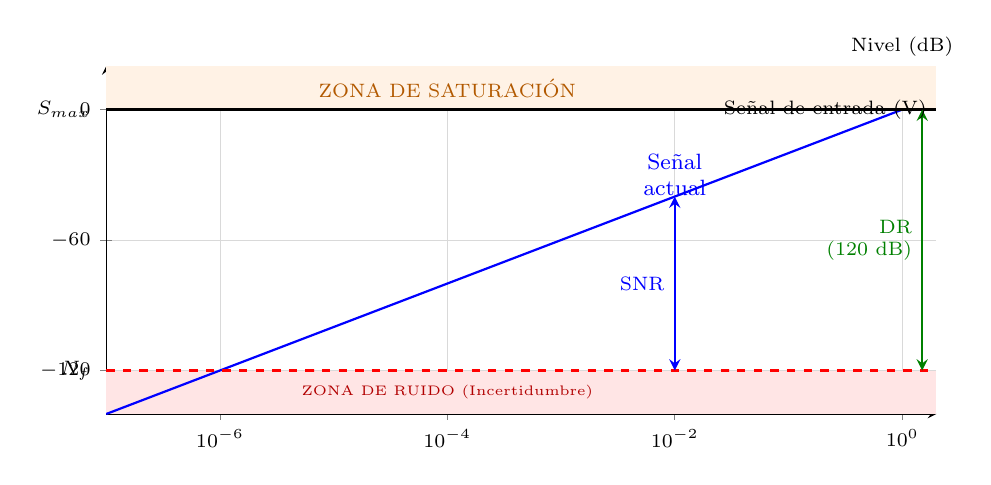
\begin{tikzpicture}
        \begin{axis}[
            width=\linewidth, height=6cm,
            xlabel={Señal de entrada (V)}, 
            ylabel={Nivel (dB)},
            xmode=log, % Escala logarítmica en X para ver décadas de voltaje
            xmin=1e-7, xmax=2,
            ymin=-140, ymax=20,
            axis lines=left,
            grid=both,
            grid style={line width=.1pt, draw=gray!10},
            major grid style={line width=.2pt,draw=gray!30},
            font=\scriptsize,
            xtick={1e-6, 1e-4, 1e-2, 1},
            ytick={-120, -60, 0},
            extra y ticks={-120, 0},
            extra y tick labels={$N_f$, $S_{max}$},
            every axis y label/.style={at=(current axis.above origin), anchor=south},
            every axis x label/.style={at=(current axis.right of origin), anchor=east},
        ]
            % 1. ZONA DE RUIDO (Sombreado)
            \fill[red!10] (axis cs:1e-7,-140) rectangle (axis cs:2,-120);
            \node[red!70!black, font=\tiny] at (axis cs:1e-4,-130) {ZONA DE RUIDO (Incertidumbre)};

            % 2. ZONA DE SATURACIÓN (Sombreado)
            \fill[orange!10] (axis cs:1e-7,0) rectangle (axis cs:2,20);
            \node[orange!70!black] at (axis cs:1e-4,10) {ZONA DE SATURACIÓN};

            % 3. CURVA DE SEÑAL
            \addplot[thick, blue, domain=1e-7:1, samples=100] {20*log10(x)};
            
            % 4. SUELO DE RUIDO (Línea horizontal)
            \addplot[thick, red, dashed, domain=1e-7:2] {-120};

            % 5. SEÑAL MÁXIMA (Línea horizontal)
            \addplot[thick, black, domain=1e-7:2] {0};

            % 6. ANOTACIÓN RANGO DINÁMICO (DR)
            \draw[<->, >=stealth, green!50!black, thick] (axis cs:1.5,-120) -- (axis cs:1.5,0) 
                node[midway, left, align=right] {DR\\(120 dB)};

            % 7. ANOTACIÓN SNR (en un punto concreto)
            \draw[<->, >=stealth, blue, thick] (axis cs:1e-2,-120) -- (axis cs:1e-2,-40) 
                node[midway, left] {SNR};
                
            \node[blue, align=center, font=\footnotesize] at (axis cs:1e-2, -30) {Señal\\actual};

        \end{axis}    
    \end{tikzpicture}        
    \caption[Diagrama de niveles de un sistema de medida.]{Diagrama de niveles de un sistema de medida. El \emph{Suelo de Ruido} ($N_f$) marca el límite inferior de detección, mientras que el nivel de \emph{Saturación} marca el límite superior. El \emph{Rango Dinámico} es una propiedad fija del sistema (\SI{120}{\decibel} en este ejemplo), mientras que la \emph{SNR} varía según la magnitud de la señal actual.}\label{fig:noise_floor}    
\end{marginfigure}

% \subsection{Resolución Real vs. Resolución Nominal}\label{sec:resolucion_real_vs_nominal}

% Es importante comprender que la resolución real de un sistema no es la que indica el número de bits del convertidor analógico a digital (ADC) o resolución nominal, sino la que impone el ruido. Si el ruido cuadrático médio o \textit{Root Mean Square} (RMS) es menor que el paso de cuantificación ($\Delta$), la resolución del sistema será la nominal y los bits menos significativos contendrán información sistemática. En cambio, si el RMS es mayor que el paso de cuantificación ($\Delta$), la resolución real del sistema estará degradada, sera inferior a la resolución nominal y los bits menos significativos solo contendrán información aleatoria.

% \begin{marginfigure}
%     \centering
%     \shorthandoff{>}
%     \begin{tikzpicture}
%         \begin{axis}[            
%             width=\linewidth, height=4.5cm,
%             xlabel={$t$}, ylabel={$y(t)$},
%             every axis y label/.style={at=(current axis.above origin),anchor=south},
%             every axis x label/.style={at=(current axis.right of origin),anchor=west},
%             axis lines=left,
%             grid=both,
%             grid style={line width=.1pt,draw=gray!10},
%             major grid style={line width=.2pt,draw=gray!30},
%             font=\scriptsize,
%             xtick={0, 1, 2, 3, 4, 5},
%             ytick={0, 0.5, 1},
%             legend style={at={(1,0.1)}, anchor=south east, font=\tiny, cells={anchor=west}}
%         ]
%             % 1. SEÑAL REAL (con ruido)
%             \addplot[thick, blue, domain=0:5, samples=200] {0.5 + 0.5*sin(deg(2*pi*0.5*x)) + 0.1*rand};
%             \addlegendentry{Señal con ruido}

%             % 2. SEÑAL NOMINAL (sin ruido)
%             \addplot[thick, red, domain=0:5, samples=200] {0.5 + 0.5*sin(deg(2*pi*0.5*x))};
%             \addlegendentry{Señal nominal}

%             % 3. PASO DE CUANTIFICACIÓN (Línea horizontal)
%             \addplot[thick, black, domain=0:5] {0.25};
%             \addlegendentry{Paso de cuantificación ($\Delta$)}

%             % 4. RESOLUCIÓN REAL            
%             \addplot[thick, green, domain=0:5, samples=200] {0.5 + 0.5*sin(deg(2*pi*0.5*x)) + 0.1*rand};
%             \addplot[thick, green, domain=0:5, samples=200] {0.5 + 0.5*sin(deg(2*pi*0.5*x))};
%             \addplot[thick, green, domain=0:5] {0.25};
%             \addlegendentry{Resolución real}

%             % 5. RESOLUCIÓN NOMINAL (Línea horizontal)
%             \addplot[thick, orange, domain=0:5] {0.0625};
%             \addlegendentry{Resolución nominal (4 bits)}
%         \end{axis}    
%     \end{tikzpicture}    
%     \caption{Resolución real vs. resolución nominal.}\label{fig:resolucion_real_vs_nominal}    
% \end{marginfigure}


\subsection{Resolución Nominal frente a Resolución Real}\label{sec:resolucion_real_vs_nominal}

En un sistema de medida digital, es fundamental distinguir entre el límite teórico impuesto por el hardware y el límite práctico impuesto por la física del ruido. La \emph{Resolución Nominal } viene determinada por el diseño del convertidor analógico a digital (ADC). Si el rango de entrada es $FS$ (\textit{Full Scale}) y el convertidor tiene $n$ bits, el paso de cuantificación $\Delta$ es:
    \begin{equation}
        \Delta = \frac{FS}{2^n}
    \end{equation}
    Este representa el \emph{peldaño} mínimo o \emph{paso de cuantificación} del sistema en ausencia total de ruido. La \emph{Resolución Real o Efectiva} es la resolución que el sistema puede alcanzar en la práctica. Depende de la relación entre el ruido cuadrático medio (\textit{Root Mean Square}, RMS) presente en la señal, $V_{n,RMS}$, y el paso de cuantificación $\Delta$.\marginnote{\textbf{Ruido \emph{pico a pico}:} Para que una medida sea estable en un display, el ruido pico a pico ($V_{pp}$) debe ser menor que $\Delta$. En una distribución gaussiana, se estima que $V_{pp} \approx 6.6 \cdot V_{n,RMS}$. Si $V_{pp} > \Delta$, los bits menos significativos oscilarán aleatoriamente, un fenómeno conocido como \textit{flicker} o parpadeo.} La variable $V_{n,RMS}$ representa el valor eficaz del ruido en la medida del cuantificador. En general, $V_{n,RMS}$ puede ser calculada con la siguiente fórmula:
    \begin{equation}
        V_{n,RMS} = \sqrt{4 k T R \Delta f}
    \end{equation}
    donde $k$ es la constante de Boltzmann, $T$ es la temperatura ambiente, $R$ es la resistencia del convertidor (o más exactamente la resistencia del sistema o resistencia equivalente de entrada) y $\Delta f$ es el ancho de banda del sistema. El ruido suelo o \textit{noise floor} es precisamente el valor de $V_{n,RMS}$, que representa el nivel mínimo de señal que el sistema puede detectar por encima del ruido inherente. Sólo una última aclaración, la ecuación del ruido cuadrático medio,  $V_{n,RMS}$, se basa en el modelo de ruido térmico (o de Johnson-Nyquist), pero en la práctica, el ruido total del sistema puede incluir otras fuentes de ruido, como el ruido de disparo, el ruido de flicker, entre otros. Por lo tanto, el valor real de $V_{n,RMS}$ puede ser mayor que el calculado solo con el ruido térmico, dependiendo de las características específicas del sistema y las condiciones de operación.

El comportamiento del sistema se puede clasificar en dos tipos de regímenes:     
\begin{enumerate}
    \item \emph{Sistema limitado por cuantificación} ($V_{n,RMS} \ll \Delta$): El ruido es tan bajo que queda \emph{escondido} dentro de un escalón de cuantificación. En este caso, la resolución real coincide con la nominal. Los bits menos significativos (\textit{Least Significant Bits}, LSB) son estables y contienen información útil de la magnitud física.
    \item \emph{Sistema limitado por ruido} ($V_{n,RMS} > \Delta$): El nivel de ruido es superior al escalón de cuantificación. La resolución real se degrada y el número efectivo de bits (ENOB, \emph{Effective Number of Bits}) es menor que el nominal ($n$). Los bits afectados por el ruido fluctúan aleatoriamente y no proporcionan información válida sobre la medida.
\end{enumerate}\marginnote{\textbf{Conclusión para el diseño:} No tiene sentido económico ni técnico utilizar un ADC de alta resolución (ej. 24 bits) si el ruido del sensor o de la etapa de acondicionamiento es muy elevado. El ingeniero debe equilibrar el suelo de ruido del hardware con la resolución del cuantificador.}

\section{Cómo se Lee una Hoja de Características}\label{sec:hoja_caracteristicas}

Todas las características anteriores acaban en una hoja de especificaciones, y leerla bien es tan importante como medir: dos instrumentos que anuncian la misma «exactitud del \SI{0.1}{\percent}» pueden comportarse de forma muy distinta según cómo esté referido ese número y en qué condiciones se haya medido. Conviene, por tanto, hacer tres preguntas a cada especificación.

\paragraph{¿Referida a la lectura o al fondo de escala?}
Una exactitud del \SI{0.1}{\percent} referida al fondo de escala es un error absoluto constante --siempre el mismo número de milivoltios--, mientras que referida a la lectura es proporcional al valor medido. La diferencia se aprecia al trabajar cerca del origen del rango, donde el error referido al fondo de escala se dispara en términos relativos:
\begin{equation}\label{eq:error_fs_lectura}
    e_{lectura} = e_{FS}\cdot\frac{\text{fondo de escala}}{\text{lectura}}
\end{equation}
de modo que un instrumento del \SI{0.1}{\percent} del fondo de escala empleado a una décima parte del rango se equivoca en un \SI{1}{\percent} de lo que indica. Por eso los multímetros de laboratorio especifican siempre dos términos: uno proporcional a la lectura y otro absoluto, con el que se cubren la deriva del cero y la resolución.

\paragraph{¿En qué condiciones?}
Toda especificación va referida a unas condiciones ambiente --habitualmente \SI{23}{\celsius} con una tolerancia de $\pm$\SI{5}{\celsius}-- y a una alimentación dadas. Fuera de ellas hay que añadir los coeficientes de las \emph{magnitudes de influencia}: la deriva térmica, en unidades por grado, y la sensibilidad a la tensión de alimentación. Ese término es el que arruina muchas medidas de campo y el que obliga a estabilizar la temperatura de una referencia o de un patrón (Capítulos~\ref{cap:metrologia} y~\ref{cap:ruido}).

\paragraph{¿Garantizada o típica?}
Un valor \emph{típico} es el que se obtiene en la mayoría de las unidades; un valor \emph{garantizado} o de peor caso es el que ninguna debe superar, y es el único que sirve para elaborar un presupuesto de errores como el de la Sección~\ref{sec:presupuesto_global}. La misma lógica se aplica a la estabilidad: una exactitud del \SI{0.01}{\percent} en veinticuatro horas puede degradarse a diez veces más en un año si el instrumento no se recalibra, de modo que el intervalo de calibración forma parte de la especificación tanto como el propio número.

La Tabla~\ref{tab:caracteristicas_medida} recoge, como resumen del capítulo, las características estudiadas, su símbolo y la forma habitual en que se especifican.

\begin{table}[ht]
    \centering
    \small
    \setlength{\tabcolsep}{3pt}
    \forcerectofloat % la tabla cae en página impar (recto); sin forzar, el caption sale al lado contrario
    \begin{tabularx}{\linewidth}{@{} L{0.24\linewidth} >{\centering\arraybackslash}X >{\centering\arraybackslash}X @{}}
        \toprule
        \textbf{Característica} & \textbf{Se especifica como} & \textbf{Dónde se estudia} \\
        \midrule
        Sensibilidad ($S$) & Pendiente de la curva de calibración: unidades de salida por unidad de entrada & Sección~\ref{sec:caract_estaticas} \\
        Linealidad & Desviación máxima respecto a la recta de referencia, en \% del fondo de escala & Sección~\ref{sec:error_no_linealidad} \\
        Histéresis y repetibilidad & Diferencia máxima entre las ramas y dispersión con entrada constante, en \% del fondo de escala & Sección~\ref{sec:histeresis_repetibilidad} \\
        Error de cero y de span ($e_0$, $\epsilon_s$) & El de cero en unidades absolutas; el de span en \% de la lectura & Sección~\ref{sub:error_cero_span} \\
        Resolución ($\Delta$) & Escalón más pequeño discernible, nominal y efectivo & Sección~\ref{sec:resolucion_real_vs_nominal} \\
        Efecto de carga & Error por la impedancia de entrada, en \% de la lectura & Sección~\ref{sub:efecto_carga_general} \\
        Prestaciones dinámicas ($t_r$, $M_p$, $t_s$, $f_c$) & Tiempos medidos sobre la respuesta al escalón y frecuencia de corte & Sección~\ref{sub:prestaciones_dinamicas} \\
        Suelo de ruido y rango dinámico ($N_f$, $DR$) & Nivel mínimo detectable y cociente con el máximo, en decibelios & Sección~\ref{sec:limites_medida} \\
        Deriva térmica & Unidades por grado centígrado, fuera de las condiciones de referencia & Sección~\ref{sec:hoja_caracteristicas} \\
        \bottomrule
    \end{tabularx}
    \caption[Características de un sistema de medida y su forma de especificarlas.]{Resumen de las características de un sistema de medida, la forma habitual de especificarlas y la sección donde se estudian. Es la lista que hay que recorrer al leer una hoja de características y la misma que se necesita, término a término, para elaborar un presupuesto de errores.\protect\label{tab:caracteristicas_medida}}
\end{table}

\section{Resumen}\label{sec:resumen_caracteristicas}

En este capítulo se ha fijado el vocabulario con el que se describe un sistema de medida, que es el que aparece después en las hojas de características, en los pliegos de condiciones y en los presupuestos de error del resto del libro:

\begin{itemize}
    \item \emph{Características estáticas} (Sección~\ref{sec:caract_estaticas}): la curva de calibración y su sensibilidad, la linealidad y la recta de referencia, la histéresis, la repetibilidad y la reproducibilidad, el rango y la saturación, y los dos defectos de la recta --error de cero y error de span (Figura~\ref{fig:errores_cero_span})--, junto con el efecto de carga, que aparece siempre que dos etapas con impedancias comparables se conectan entre sí.
    \item \emph{Características dinámicas} (Sección~\ref{sec:caract_dinamicas}): la respuesta al escalón de los sistemas de orden cero, primero y segundo, con la constante de tiempo, la frecuencia natural y el amortiguamiento como parámetros; y las prestaciones con las que se especifican --tiempo de subida, sobreoscilación máxima, tiempo de establecimiento y ancho de banda (Figura~\ref{fig:prestaciones_dinamicas})--, con $\zeta \approx 0{,}7$ como el compromiso recomendado entre rapidez y estabilidad.
    \item \emph{Límites de la medida} (Sección~\ref{sec:limites_medida}): el suelo de ruido, el rango dinámico y la relación señal-ruido, junto con la diferencia entre resolución nominal y resolución real (Figura~\ref{fig:noise_floor}), que es lo que fija hasta dónde se puede medir y no solo qué se puede medir.
    \item \emph{Cómo se lee una hoja de características} (Sección~\ref{sec:hoja_caracteristicas}): si la especificación está referida a la lectura o al fondo de escala (ecuación~\eqref{eq:error_fs_lectura}), en qué condiciones de referencia se ha medido, si el valor es típico o garantizado y qué magnitudes de influencia hay que añadir en cada caso; la Tabla~\ref{tab:caracteristicas_medida} reúne todas las características del capítulo con su forma de especificarlas.
\end{itemize}

\marginnote{\textbf{Conclusión:} ninguna de las características de este capítulo se puede mejorar más adelante. La exactitud de un sistema de medida queda fijada cuando se eligen el sensor y su acondicionamiento, y lo que hace el resto del libro es conservarla: digitalizarla sin degradarla (Capítulo~\ref{cap:daq}), protegerla del entorno (Capítulo~\ref{cap:ruido}) y transmitirla sin perderla (Capítulo~\ref{cap:buses}).}

% !TeX root = main.tex
% !TEX program = pdflatex

\chapter{Sensores Resistivos}

En este capítulo se estudian los sensores cuyo principio de funcionamiento se basa en la variación de la resistencia eléctrica ($\Delta R$) ante cambios en una magnitud física. Analizaremos desde el modelado físico de potenciómetros y galgas hasta la caracterización de sensores de temperatura (RTD y termistores) y luz (LDR), prestando especial atención a los efectos de carga y las configuraciones de conexión industrial.

\section{Principios Físicos de la Conversión Resistiva}\label{sec:fundamentos_resistivos}

La resistencia de un conductor viene definida por su geometría y su resistividad:
\begin{equation}
    R = \rho \frac{L}{A}
\end{equation}
donde $\rho$ es la resistividad, $L$ la longitud y $A$ el área de la sección transversal. Los sensores resistivos aprovechan la variación de estos parámetros ante estímulos externos:
\begin{itemize}
    \item \emph{Variación geométrica ($\Delta L, \Delta A$)}: Potenciómetros y galgas extensiométricas.
    \item \emph{Variación de resistividad ($\Delta \rho$)}: RTDs, termistores, LDRs y magnetorresistencias.
\end{itemize}
La Figura~\ref{fig:resistencia} ilustra la variación de la resistencia ante cambios en la geometría y la resistividad. En la Figura \ref{fig:resistencia}a se muestra cómo un potenciómetro varía su resistencia al deslizar un contacto móvil, mientras que en la Figura~\ref{fig:resistencia}b se observa cómo una galga extensiométrica cambia su resistencia al estirarse o comprimirse.

\begin{marginfigure}
    \centering
    \shorthandoff{>}
    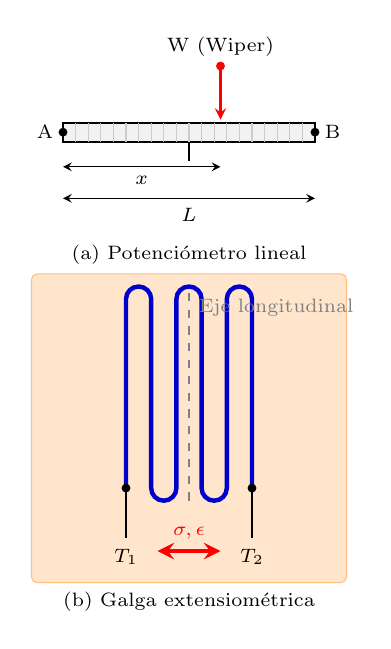
\begin{tikzpicture}[scale=0.8, font=\scriptsize]
        % --- DIBUJO A: POTENCIÓMETRO ---
        \begin{scope}[yshift=0cm]
            % Pista resistiva (rectángulo sombreado)
            \draw[fill=gray!10, thick] (0,0) rectangle (4,0.3);
            \foreach \x in {0.2,0.4,...,3.8} \draw[gray!40] (\x,0) -- (\x,0.3);
            
            % Terminales fijos
            \fill (0,0.15) circle (2pt) node[left] {A};
            \fill (4,0.15) circle (2pt) node[right] {B};
            
            % Contacto móvil (Wiper)
            \draw[thick, red, -stealth] (2.5, 1.2) -- (2.5, 0.35);
            \fill[red] (2.5, 1.2) circle (2pt) node[above, black] {W (Wiper)};
            
            % Cotas de posición
            \draw[<->, >=stealth] (0,-0.4) -- (2.5,-0.4) node[midway, below] {$x$};
            \draw[<->, >=stealth] (0,-0.9) -- (4,-0.9) node[midway, below] {$L$};
            
            % Poner en el centro la etiqueta Potenciometro lineal
            \draw[thick] (2,0) -- (2,-0.3);  
            \node at (2,-1.8) {(a) Potenciómetro lineal};
        \end{scope}

        % --- DIBUJO B: GALGA EXTENSIOMÉTRICA ---
        \begin{scope}[yshift=-5.5cm]
            % Base de la galga (Poliamida)
            \draw[fill=orange!20, draw=orange!50, rounded corners=2pt] (-0.5,-1.5) rectangle (4.5, 3.4);
            
            % Rejilla metálica (Serpentín)
            \draw[ultra thick, blue!80!black] 
                (1,0) -- (1,3) 
                arc(180:0:0.2) -- (1.4,0) 
                arc(-180:0:0.2) -- (1.8,3) 
                arc(180:0:0.2) -- (2.2,0) 
                arc(-180:0:0.2) -- (2.6,3) 
                arc(180:0:0.2) -- (3.0,0);
            
            % Terminales de conexión
            \draw[thick] (1,0) -- (1,-0.8) node[below] {$T_1$};
            \draw[thick] (3.0,0) -- (3.0,-0.8) node[below] {$T_2$};
            \fill (1,0) circle (2pt);
            \fill (3.0,0) circle (2pt);
            
            % Eje de deformación (Esfuerzo)
            \draw[<->, >=stealth, red, ultra thick] (1.5, -1) -- (2.5, -1) node[midway, above] {$\sigma, \epsilon$};
            \draw[dashed, gray] (2, -0.2) -- (2, 3.2) node[pos=0.9, right] {Eje longitudinal};
            
            \node at (2,-1.8) {(b) Galga extensiométrica};
        \end{scope}
    \end{tikzpicture}
    \caption{Representación física de sensores resistivos: (a) Potenciómetro donde la posición $x$ del cursor determina la división de tensión a través del wiper. (b) Galga extensiométrica donde la deformación longitudinal $\epsilon$ altera la resistencia del hilo metálico $\sigma$.}\label{fig:resistencia}
\end{marginfigure}



\section{Potenciómetros de Medida}\label{sec:potenciometros}

En esta sección se analiza el funcionamiento de los potenciómetros como sensores de posición. Se estudia su modelo ideal, la influencia de la carga externa (efecto de carga) y cómo esto afecta la linealidad de la medida.

\subsection{Modelo Ideal y Resolución}

El potenciómetro ideal se modela como una resistencia variable $R(x) = R_{total} \frac{x}{L}$, donde $x$ es la posición del cursor y $L$ la longitud total de la pista resistiva. La salida de tensión por el cursor se obtiene mediante un divisor de tensión: 
\begin{equation}
    V_{out} = V_{in} \frac{R(x)}{R(x) + R_L}
\end{equation}
donde $R_L$ es la resistencia de carga conectada a la salida. En el caso ideal sin carga ($R_L \to \infty$), la salida es lineal con la posición: $V_{out} = V_{in} \frac{x}{L}$.


\subsection{Efecto de Carga y Error de Linealidad}\label{sec:efecto_carga}
% Aquí desarrollaremos el análisis de cómo RL afecta a la medida.
Cuando se conecta una carga $R_L$ a la salida del potenciómetro, el divisor de tensión ya no es ideal y la salida se ve afectada por el efecto de carga, como se muestra en la Figura~\ref{fig:efecto_carga}. La relación entre la salida real y la posición se vuelve no lineal, especialmente cuando $R_L$ es bastante menor que $R(x)$. El error de linealidad introducido por el efecto de carga se puede cuantificar como:
\begin{equation}
    \text{Error} = \frac{V_{out} - V_{ideal}}{V_{ideal}} = \frac{V_{in} \frac{R(x)}{R(x) + R_L} - V_{in} \frac{x}{L}}{V_{in}}
\end{equation}  
\marginnote{\textbf{Efecto de carga:} El efecto de carga es un fenómeno que ocurre cuando la resistencia de carga $R_L$ conectada a la salida del potenciómetro es lo suficientemente baja como para afectar la tensión de salida. Esto provoca una desviación de la respuesta ideal, introduciendo un error de linealidad que se vuelve más pronunciado a medida que $R_L$ disminuye. En aplicaciones donde se requiere alta precisión, es crucial minimizar este efecto utilizando amplificadores de alta impedancia o seleccionando potenciómetros con resistencias totales significativamente mayores que la resistencia de carga.} 
%Figura que ilustra el efecto de carga en la respuesta del potenciómetro, mostrando cómo la salida se desvía de la linealidad ideal a medida que $R_L$ disminuye.
% \begin{marginfigure}
%     \centering
%     \shorthandoff{>}
%     \begin{tikzpicture}
%         \draw[thick] (0,0) -- (4,0);
%         \draw[thick] (0,0) -- (0,2);
%         \draw[thick] (0,2) -- (4,2);
%         \draw[thick] (4,0) -- (4,2);
%         \draw[thick] (2,0) -- (2,2);        
%         \fill (0,0) circle (2pt);        
%         \fill (4,0) circle (2pt);        
%         \fill (0,2) circle (2pt);        
%         \fill (4,2) circle (2pt);        
%         \draw[thick, red, -stealth] (0.5, 1.5) -- (1.5, 0.5) node[midway, above] {$R_L$};
%         \draw[thick, blue, -stealth] (2.5, 1.5) -- (3.5, 0.5) node[midway, above] {$R(x)$};
%         \node at (2, -0.5) {Posición $x$};
%         \node at (2, 2.5) {Tensión de salida $V_{out}$};
%         \node at (2, 1) {Respuesta ideal sin carga};
%         \node at (2, 0.5) {Respuesta con carga $R_L$};
%     \end{tikzpicture}
%     \caption{Ilustración del efecto de carga en un potenciómetro. La curva azul representa la respuesta ideal sin carga, mientras que la curva roja muestra cómo la salida se desvía de la linealidad ideal a medida que la resistencia de carga $R_L$ disminuye.}\label{fig:efecto_carga}
% \end{marginfigure}

El error de linealidad absoluto se define como la diferencia entre la salida real y la ideal: $\epsilon = V_{o,real} - V_{o,ideal}$. El error relativo máximo ocurre aproximadamente en $k \approx 0.67$ (2/3 del recorrido) y se puede aproximar por:
\begin{equation}
    \epsilon_{\max} \approx \frac{4}{27} \frac{R_t}{R_L} \times 100\%
\end{equation}

\begin{marginfigure}[2em]
    \centering
    \shorthandoff{>}
    % --- ESQUEMA DEL CIRCUITO ---
    \begin{tikzpicture}[scale=1]
        % Fuente y Potenciómetro
        \draw (0,0) node[ground]{} to[V, v=$V_i$] (0,3) -- (2,3);
        \draw (2,3) to[R, l=$R_1$] (2,1.5) coordinate (wiper);
        \draw (wiper) to[R, l=$R_2$] (2,0) node[ground]{};
        
        % Conexión a Carga
        \draw (wiper) -- (3.5,1.5) to[R, l=$R_L$] (3.5,0) node[ground]{};
        \draw (3.5,1.5) to[short, -o] (4,1.5) node[right] {$V_o$};
        
        % Etiquetas de resistencia
        \node[left, font=\tiny] at (1.75,2.25) {$(1-k)R_t$};
        \node[left, font=\tiny] at (1.75,0.75) {$k R_t$};
    \end{tikzpicture}
    
    \vspace{1cm}
    
    % --- GRÁFICA DE ERROR ---
    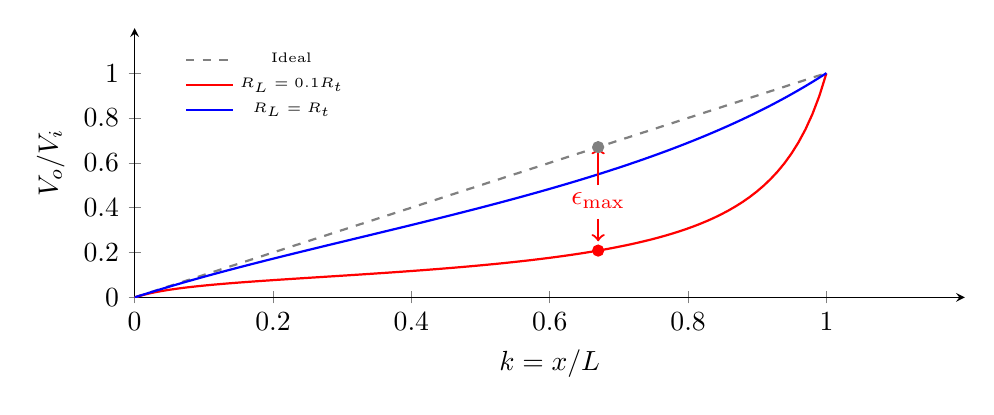
\begin{tikzpicture}
        \begin{axis}[
            width=\linewidth, height=5cm,
            xlabel={$k = x/L$}, ylabel={$V_o/V_i$},
            xmin=0, xmax=1.2, ymin=0, ymax=1.2,
            ytick={0, 0.2, 0.4, 0.6, 0.8, 1}, 
            xtick={0, 0.2, 0.4, 0.6, 0.8, 1},
            %font=\tiny,
            axis lines=left,
            legend style={at={(0.05,0.95)}, anchor=north west, draw=none, font=\tiny}
        ]
            % Respuesta Ideal (Recta)
            \addplot[thick, gray, dashed, domain=0:1] {x};
            \addlegendentry{Ideal};

            % Respuesta con Carga (Rt/RL = 10 para que se note mucho)
            % Formula: x / (1 + x*(1-x)*10)
            \addplot[thick, red, domain=0:1, samples=100] {x / (1 + x*(1-x)*10)};
            \addlegendentry{$R_L = 0.1 R_t$};
            
            % Respuesta con Carga (Rt/RL = 1)
            \addplot[thick, blue, domain=0:1, samples=100] {x / (1 + x*(1-x)*1)};
            \addlegendentry{$R_L = R_t$};
            
            % Marcar el punto de error máximo
            \addplot[only marks, mark=*, red] coordinates {(0.67,{0.67 / (1 + 0.67*(1-0.67)*10)})};
            % ahora sobre la recta ideal
            \addplot[only marks, mark=*, gray] coordinates {(0.67,0.67)};

            \node[red] at (axis cs:0.67,0.43) {$\epsilon_{\max}$};
            % Dibujar una flecha para indicar el error máximo
            \draw[->, thick, red] (axis cs:0.67,0.35) -- (axis cs:0.67,0.25);
            \draw[->, thick, red] (axis cs:0.67,0.5) -- (axis cs:0.67,0.67);

        \end{axis}
    \end{tikzpicture}
    \caption{Efecto de carga. El circuito (arriba) muestra la $R_L$ en paralelo con el brazo inferior. La gráfica (abajo) ilustra cómo la salida se \emph{aplasta} respecto a la ideal, perdiendo linealidad. El eje $y$ representa la relación $V_o/V_i$ y el eje $x$ la posición del cursor.}\label{fig:efecto_carga}
\end{marginfigure}

Ese error se vuelve significativo cuando $R_L$ es pequeño, lo que reduce la resolución efectiva del potenciómetro. Para minimizar este efecto, se recomienda utilizar un amplificador de alta impedancia de entrada o seleccionar un potenciómetro con una resistencia total $R_{total}$ mucho mayor que la resistencia de carga $R_L$. Se utiliza un amplificador operacional en configuración seguidor de tensión para asegurar que la carga no afecte la medida, manteniendo la linealidad y precisión del potenciómetro. eso es debido a que el seguidor de tensión presenta una impedancia de entrada muy alta, lo que minimiza el efecto de carga y permite obtener una salida que sigue fielmente la tensión en el cursor del potenciómetro.

\section{Galgas Extensiométricas (\textit{Strain Gauges})}\label{sec:galgas}

Se estudia el comportamiento de las galgas extensiométricas como sensores de deformación. Se analiza el factor de galga, los tipos de galgas (metálicas y de semiconductor) y cómo la temperatura afecta su respuesta, así como las técnicas de compensación para mitigar estos efectos. Se discuten también las aplicaciones industriales de las galgas en la medición de esfuerzos y deformaciones en estructuras.\marginnote{\textbf{Ejercicio para clase:} 
    Si tenemos un potenciómetro de \SI{10}{\kilo\ohm} y queremos que el error de linealidad por efecto de carga sea inferior al \SI{0.5}{\%}, ¿cuál debe ser la resistencia mínima del sistema de adquisición?     
    \textit{Solución: $R_L > \SI{296}{\kilo\ohm}$.}
}

\subsection{El Factor de Galga ($G$)}
Una galga es un sensor que mide la deformación ($\epsilon$) a través de la variación de su resistencia ($\Delta R$). El factor de galga se define como:
\begin{equation}
    G = \frac{\Delta R / R}{\epsilon}
\end{equation}
Este factor depende del material y la geometría de la galga. Para galgas metálicas típicas, $G \approx 2$, mientras que para galgas de semiconductor puede ser mucho mayor, llegando a valores de $G \approx 100$ o más, debido a la fuerte dependencia de la resistividad con la deformación. La Figura~\ref{fig:factor_galga} muestra la relación entre la deformación y la variación de resistencia para diferentes tipos de galgas, destacando cómo las galgas de semiconductor presentan una respuesta mucho más sensible a la deformación en comparación con las galgas metálicas.

% \begin{marginfigure}
%     \centering
%     \shorthandoff{>}
%     \begin{tikzpicture}
%         \begin{axis}[
%             width=\linewidth, height=5cm,
%             xlabel={Deformación $\epsilon$}, ylabel={Variación de Resistencia $\Delta R / R$},
%             xmin=0, xmax=0.01, ymin=0, ymax=1.0,
%             ytick={0, 0.2, 0.4, 0.6, 0.8, 1.0}, 
%             xtick={0, 0.0025, 0.005, 0.0075, 0.01},
%             axis lines=left,
%             legend style={at={(0.05,0.95)}, anchor=north west, draw=none, font=\tiny}
%         ]
%             % Galga Metálica (G ~ 2)
%             \addplot[thick, blue] {2*x};
%             \addlegendentry{G = 2 (Metálica)};

%             % Galga de Semiconductor (G ~ 100)
%             \addplot[thick, red] {100*x};
%             \addlegendentry{G = 100 (Semiconductor)};
%         \end{axis}
%     \end{tikzpicture}
%     \caption{Relación entre la deformación $\epsilon$ y la variación de resistencia $\Delta R / R$ para galgas metálicas y de semiconductor. Las galgas de semiconductor muestran una respuesta mucho más sensible a la deformación en comparación con las galgas metálicas debido a su mayor factor de galga $G$.}\label{fig:factor_galga}
% \end{marginfigure}

\begin{marginfigure}
    \centering
    \shorthandoff{>}
    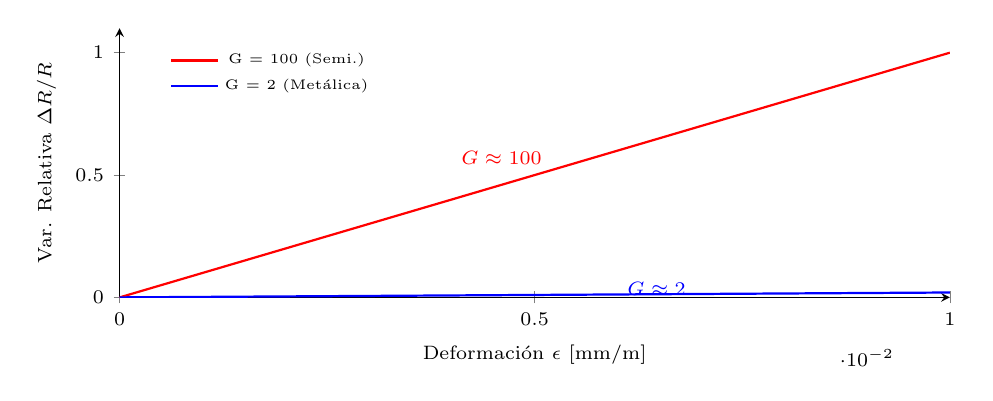
\begin{tikzpicture}
        \begin{axis}[
            width=\linewidth, height=5cm,
            xlabel={Deformación $\epsilon$ [mm/m]}, 
            ylabel={Var. Relativa $\Delta R / R$},
            % Definimos el dominio para que coincida con la vista
            xmin=0, xmax=0.01, 
            ymin=0, ymax=1.1,
            % Formato de números para evitar notación científica amontonada
            xtick={0, 0.005, 0.01},
            xticklabel style={/pgf/number format/fixed, /pgf/number format/precision=3},
            axis lines=left,
            font=\scriptsize,
            legend style={at={(0.05,0.95)}, anchor=north west, font=\tiny, draw=none}
        ]
            % Galga de Semiconductor (G = 100)
            % IMPORTANTE: domain=0:0.01 evita el error "Dimension too large"
            \addplot[thick, red, domain=0:0.01, samples=2] {100*x};
            \addlegendentry{G = 100 (Semi.)};

            % Galga Metálica (G = 2)
            \addplot[thick, blue, domain=0:0.01, samples=2] {2*x};
            \addlegendentry{G = 2 (Metálica)};

            % Nodo explicativo
            \node[red, anchor=south west] at (axis cs:0.004, 0.5) {$G \approx 100$};
            \node[blue, anchor=north west] at (axis cs:0.006, 0.1) {$G \approx 2$};
        \end{axis}
    \end{tikzpicture}
    \caption[Comparativa de sensibilidad entre galgas.]{Comparativa de sensibilidad entre galgas. Nótese que para una deformación de \qty{0.01}{mm/m}, la galga metálica apenas varía un \qty{2}{\percent}, mientras que la de semiconductor llega al \qty{100}{\percent} de variación ($\Delta R = R$).}\label{fig:factor_galga}
\end{marginfigure}

\subsection{Tipos de Galgas: Metálicas y de Semiconductor}
Las galgas metálicas están hechas de aleaciones como Constantán o Karma, que tienen un factor de galga relativamente bajo pero son estables y lineales con la temperatura. Las galgas de semiconductor, por otro lado, utilizan materiales como silicio o germanio, que presentan una alta sensibilidad debido a su fuerte dependencia de la resistividad con la deformación. Sin embargo, las galgas de semiconductor son más susceptibles a la temperatura, poco lineales y requieren técnicas de compensación para mantener la precisión en aplicaciones industriales.

%Usos
Las galgas extensiométricas metálicas se utilizan comúnmente en aplicaciones de ingeniería civil y mecánica para medir esfuerzos en puentes, edificios y maquinaria. Las galgas de semiconductor, debido a su alta sensibilidad, se emplean en aplicaciones donde se requieren mediciones de deformación extremadamente precisas, como en la investigación científica y en la industria aeroespacial.

%MEMS
Las galgas de semiconductor se han miniaturizado en forma de dispositivos MEMS (\textit{Microelectromechanical Systems}), que integran sensores de deformación con circuitos electrónicos en un solo chip, permitiendo aplicaciones avanzadas en monitoreo estructural y biomecánica. Un ejemplo de MEMS es el acelerómetro piezoresistivo como el que semuestra en la Figura~\ref{fig:mems_acelerometro}, que utiliza galgas de semiconductor para medir la aceleración a través de la deformación inducida en las estructuras del dispositivo que como máximo ejempo es el acelerómetro del teléfono móvil, que detecta la orientación del dispositivo y permite funciones como el cambio automático entre modo vertical y horizontal. Las galgas de semiconductor muestran una respuesta mucho más sensible a la deformación en comparación con las galgas metálicas debido a su mayor factor de galga $G$. Las galgas son regiones del propio silicio de la viga que han sido dopadas selectivamente (es decir, con impurezas mediante un proceso de difusion o implantación iónica) para ser piezorresistivas.\marginnote{\textbf{Dopaje y Orientación Cristalina:} El efecto piezorresistivo en el silicio es anisotrópico (depende de la dirección). Dopaje tipo P (Boro): Es el más utilizado en MEMS. Se introducen átomos de Boro (trivalentes) que crean \emph{huecos}. El silicio tipo P es extremadamente sensible a los esfuerzos de cizalla en la dirección cristalográfica <110>, que es la dirección estándar de los brazos en un acelerómetro. Dopaje tipo N (Fósforo/Arsénico): Se introducen electrones en exceso. Aunque también es piezorresistivo, su coeficiente de sensibilidad suele ser menor que el del tipo P para la mayoría de las configuraciones. Existe un compromiso con la catidad de dopaje. Bajo Dopaje: Si ponemos pocos átomos de Boro, el sensor es muy sensible (Factor de Galga $G$ muy alto), pero es inestable con la temperatura. Cualquier cambio térmico altera la resistencia tanto como la deformación. Alto Dopaje (Silicio Degenerado): Si saturamos el silicio con mucho Boro, el sensor se vuelve muy estable térmicamente, pero pierde mucha sensibilidad (el Factor de Galga $G$ baja). La Figura~\ref{fig:zona_dopada} muestra la integración de la galga de semiconductor en el acelerómetro piezoresistivo. Lo que hace que el dopaje sea piezorresistivo es que las impurezas permiten que los cambios en la red cristalina afecten directamente a la nube de electrones/huecos, algo que en un aislante o en un conductor metálico normal no ocurre con tanta intensidad.
} Se colocan sobre la superficie de la viga, lo más cerca posible de las uniones (con el marco, que tambien es de silicio fijo). Si imaginamos la viga como una tabla de trampolín, cuando la masa se mueve, la viga se dobla. El punto donde el silicio se estira y se comprime más (máximo esfuerzo mecánico) es justo en el \emph{encastre}, es decir, donde la viga nace del marco fijo (y también donde se une a la masa). De hecho, para un acelerómetro de alta calidad (puente completo), se suelen poner galgas en ambos extremos de cada viga (una cerca del marco y otra cerca de la masa).

%Figura de un MEMS del acelerómetro piezoresistivo, mostrando cómo las galgas de semiconductor están integradas en la estructura del dispositivo para medir la aceleración a través de la deformación inducida.
\begin{marginfigure}
    \centering
    \shorthandoff{>}
    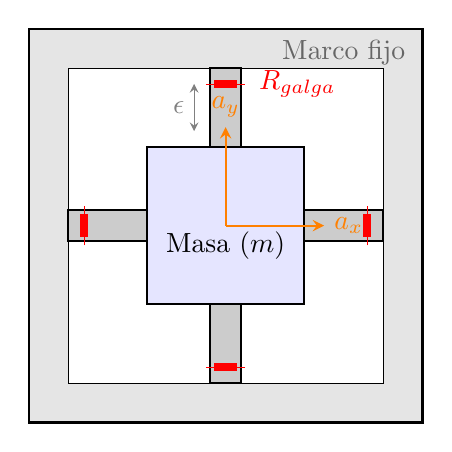
\begin{tikzpicture}[scale=1]
        % Marco exterior (Sustrato de silicio fijo)
        \draw[thick, fill=gray!20] (-2.5,-2.5) rectangle (2.5,2.5);
        \draw[fill=white] (-2,-2) rectangle (2,2); % Hueco grabado
        
        % Masa sísmica (Proof Mass)
        \draw[thick, fill=blue!10] (-1,-1) rectangle (1,1);
        \node at (0,-0.25) {Masa ($m$)};
        
        % Brazos de suspensión (Vigas/Flexures)
        % Arriba
        \draw[thick, fill=gray!40] (-0.2,1) rectangle (0.2,2);
        % Abajo
        \draw[thick, fill=gray!40] (-0.2,-1) rectangle (0.2,-2);
        % Izquierda
        \draw[thick, fill=gray!40] (-1,-0.2) rectangle (-2,0.2);
        % Derecha
        \draw[thick, fill=gray!40] (1,-0.2) rectangle (2,0.2);
        
        % Galgas piezorresistivas (Semiconductoras)
        % Se colocan en los puntos de máximo esfuerzo (unión viga-marco)
        \foreach \x/\y/\r in {0/1.8/0, 0/-1.8/0, -1.8/0/90, 1.8/0/90} {
            \begin{scope}[shift={(\x,\y)}, rotate=\r]
                \fill[red] (-0.15,-0.05) rectangle (0.15,0.05);
                \draw[red, ultra thin] (-0.25,0) -- (0.25,0); % Contactos
            \end{scope}
        }
        
        % Leyendas y etiquetas
        \node[red, anchor=west] at (0.3, 1.8) {$R_{galga}$};
        \node[gray!80!black] at (1.5, 2.2) {Marco fijo};
        
        % Ejes de sensibilidad
        \draw[thick, -stealth, orange] (0,0) -- (0,1.25) node[above] {$a_y$};
        \draw[thick, -stealth, orange] (0,0) -- (1.25,0) node[right] {$a_x$};
        
        % Detalle de flexión
        \draw[<->, >=stealth, gray] (-0.4, 1.2) -- (-0.4, 1.8) node[midway, left] {$\epsilon$};

    \end{tikzpicture}
    \caption[Estructura de un acelerómetro MEMS.]{Estructura de un acelerómetro MEMS. La aceleración desplaza la masa central, deformando las vigas de suspensión. Las galgas de semiconductor (en rojo) integradas en las zonas de máxima flexión detectan la deformación $\epsilon$. El silicio tiene excelentes propiedades mecánicas (no presenta histéresis elástica y es casi tan duro como el acero), lo que permite fabricar sensores de aceleración extremadamente robustos y de bajo coste. }\label{fig:mems_acelerometro}
\end{marginfigure}

\begin{marginfigure}[0em]
    \centering
    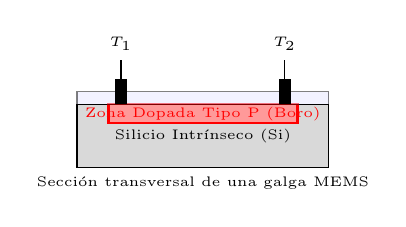
\begin{tikzpicture}[scale=0.8, font=\tiny]
        % Sustrato de Silicio (Bulk)
        \draw[fill=gray!30] (0,0) rectangle (4,1);
        \node at (2,0.5) {Silicio Intrínseco (Si)};
        
        % Zona Dopada (La galga)
        \draw[fill=red!40, draw=red, thick] (0.5,0.7) rectangle (3.5,1);
        \node[red] at (2,0.85) {Zona Dopada Tipo P (Boro)};
        
        % Capa de Pasivación (Óxido)
        \draw[fill=blue!10, opacity=0.5] (0,1) rectangle (4,1.2);
        
        % Contactos de Aluminio
        \fill[black] (0.6,1) rectangle (0.8,1.4);
        \fill[black] (3.2,1) rectangle (3.4,1.4);
        \draw (0.7,1.4) -- (0.7,1.7) node[above] {$T_1$};
        \draw (3.3,1.4) -- (3.3,1.7) node[above] {$T_2$};
        
        \node[below] at (2,0) {Sección transversal de una galga MEMS};

        % Vista de planta

    \end{tikzpicture}
    \caption{Integración de la galga en el silicio. La zona roja es la que cambia su resistividad ante la flexión del sustrato.}\label{fig:zona_dopada}
\end{marginfigure}

Ante una aceleración externa $\vec{a}$, la masa central experimenta una fuerza inercial $\vec{F}=m\vec{a}$. Esta fuerza provoca el desplazamiento de la masa, lo que genera una flexión en las vigas de suspensión. Según la teoría de vigas, el esfuerzo máximo ($\sigma$) se produce en la unión de las vigas con el marco fijo formado por un sustrato de silicio fijo. Las galgas de semiconductor situadas en estos puntos críticos aprovechan su elevado Factor de Galga ($G \approx 100$) para convertir la deformación en una variación de resistencia significativa ($\Delta R/R = G \cdot \epsilon \approx 0.1$). Normalmente, estas cuatro galgas se conectan en una configuración de puente de Wheatstone completo para maximizar la sensibilidad y compensar efectos térmicos no deseados.

\subsection{Influencia de la Temperatura y Compensación}
La temperatura afecta tanto a las galgas metálicas como a las de semiconductor, aunque de manera diferente. En las galgas metálicas, la resistencia varía con la temperatura debido al coeficiente de temperatura de la resistividad ($\alpha$), lo que puede introducir errores en la medida de deformación. En las galgas de semiconductor, la dependencia de la resistividad con la temperatura es aún más pronunciada, lo que puede resultar en errores significativos si no se compensa adecuadamente. Para mitigar estos efectos, se utilizan técnicas de compensación como la conexión en puente de Wheatstone, donde se combinan galgas activas (sujetas a deformación) con galgas de referencia (no deformadas) para cancelar las variaciones debidas a la temperatura. Además, se pueden emplear materiales con bajo coeficiente de temperatura o implementar algoritmos de corrección basados en mediciones de temperatura para mejorar la precisión de las galgas en entornos variables.

\section{Sensores de Temperatura Resistivos (RTD)}\label{sec:rtd}




\subsection{Metales Utilizados: El platino y la Pt100}
\subsection{Ecuación de Callendar-Van Dusen}
\subsection{Configuraciones de Conexión: 2, 3 y 4 hilos}\label{sec:conexion_hilos}
% Vital para instrumentación industrial.
\subsection{Error por Autocalentamiento}

\section{Termistores (NTC y PTC)}\label{sec:termistores}

\subsection{Termistores NTC: Modelo Exponencial y Parámetro $\beta$}
\subsection{Ecuación de Steinhart-Hart}
\subsection{Linealización de la Respuesta NTC}
\subsection{Termistores PTC y aplicaciones de protección}

\section{Sensores de Luz y Campos Magnéticos}\label{sec:otros_resistivos}

\subsection{Fotorresistencias (LDR): Respuesta Espectral}
\subsection{Magnetorresistencias (AMR y GMR)}

\section{Circuitos de Medida: El Puente de Wheatstone}\label{sec:puente_wheatstone}

\subsection{Análisis del Puente Desequilibrado}
\subsection{Configuraciones: Cuarto, Medio y Puente Completo}
\subsection{Linealidad según el tipo de excitación (Voltaje vs. Corriente)}

\section{Resumen de Errores en Sensores Resistivos}\label{sec:errores_resistivos}
% !TeX root = main.tex
% !TEX program = pdflatex

\chapter{Sensores Reactivos: Capacitivos e Inductivos}\label{cap:reactivos}

En este capítulo se estudian los sensores basados en la variación de los parámetros reactivos de un circuito: la capacidad ($C$) y la inductancia ($L$). Estos sensores destacan por su alta resolución, ausencia de contacto físico y versatilidad. Analizaremos sus modelos físicos, el impacto crítico de las capacidades parásitas y las técnicas de acondicionamiento en alterna necesarias para convertir variaciones de impedancia en señales de tensión procesables.


\section{Fundamentos de los Sensores Reactivos}\label{sec:fundamentos_reactivos}

A diferencia de los sensores resistivos que disipan energía, los sensores reactivos la almacenan en campos eléctricos o magnéticos. Puesto que en corriente continua un condensador ideal es un circuito abierto y un inductor un cortocircuito, la medida de estos sensores exige el uso de una señal de \emph{excitación alterna} ($v_{exc} = V_p \sin(\omega t)$). La magnitud física a medir altera la geometría o las propiedades electromagnéticas del sensor, modificando su reactancia $X$:
\begin{equation}
    X_C = \frac{1}{j\omega C} \quad ; \quad X_L = j\omega L
\end{equation}

En el estudio de los sensores reactivos, la oposición al paso de la corriente alterna se describe mediante la \emph{Impedancia compleja ($\mathit{Z}$)}. Esta magnitud unifica el comportamiento disipativo de la resistencia ($R$) con el comportamiento de almacenamiento de energía de la reactancia ($X$):

\begin{equation}
    Z = R + jX
\end{equation}

Donde $R$ es la parte real y $X$ es la parte imaginaria. Como se ilustra en la Figura~\ref{fig:impedancia_compleja}, el signo de la reactancia determina el carácter del sensor:

\begin{itemize}
    \item \emph{Carácter Inductivo}: La reactancia es positiva ($X_L = \omega L$). La tensión adelanta a la corriente.
    \item \emph{Carácter Capacitivo}: La reactancia es negativa ($X_C = -1/\omega C$). La corriente adelanta a la tensión.
\end{itemize}

\begin{marginfigure}[0em]
    \centering
    \shorthandoff{>}
    \begin{tikzpicture}[american, scale=1]
        \ctikzset{resistors/scale=0.7, inductors/scale=0.7, inductor=cute, capacitors/scale=0.7}

        % --- PARTE 1: PLANO COMPLEJO GENERAL ---
        \begin{scope}
            % Ejes
            \draw[->, >=stealth] (-1.5,0) -- (2.5,0) node[below] {Real};
            \draw[->, >=stealth] (0,-1.5) -- (0,2) node[left] {Imaginario};
            
            % Vectores
            \draw[ultra thick, white!40!black,-stealth] (0.2,0.1) -- (1.5,0.1) node[right, above] {$R$};
            \draw[ultra thick, green!60!black, -stealth] (-0.1,0.2) -- (-0.1,1.5) node[left] {$X_L$};
            \draw[ultra thick, blue!60!black, -stealth] (-0.1,-0.2) -- (-0.1,-1.2) node[left] {$X_C$};
            
            % Fórmulas
            \node[anchor=west] at (1.2, 1.5) {$X_L = j\omega L$};
            \node[anchor=west] at (1.2, -1.0) {$X_C = \dfrac{-j}{\omega C} = \dfrac{1}{j\omega C}$};
            
            % Iconos
            \draw (-1.2, 1.2) to[L, color=red] (-1.2, 0.2); \node[left, red] at (-1.2, 0.7) {$L$};
            \draw (-1.2, -0.2) to[C, color=red] (-1.2, -1.2); \node[left, red] at (-1.2, -0.7) {$C$};
            \draw(0.4, 0.7) to[R, color=red] (1.4, 0.7); \node[left, red] at (1.2, 1.1) {$R$};
        \end{scope}

        % --- PARTE 2: CIRCUITO RL ---
        \begin{scope}[xshift=-1cm, yshift=-3.5cm]
            %\draw[dotted] (-1.8, 2) rectangle (4.5, -0.5);
            % Diagrama fasorial
            \draw[->] (-0.2,0) -- (2,0) node[below] {$R_L$};
            \draw[->] (0,-0.2) -- (0,1.5);
            \draw[thick, -stealth] (0,0) -- (1.5,0); % R
            \draw[thick, green!60!black, -stealth] (1.5,0) -- (1.5,1.2) node[right] {$j\omega L$};
            \draw[thick, blue, -stealth] (0,0) -- (1.5,1.2) node[midway, above left] {$Z_L$};
            
            % Circuito y Fórmula
            \begin{scope}[xshift=2.5cm, yshift=1cm]
                \draw[red] (0,0) to[R, l=$R_L$] (0.8,0) to[L, l=$L$] (1.6,0);
                \node[anchor=north] at (0.8, -0.2) {$Z_L = R_L + j\omega L$};
            \end{scope}
        \end{scope}

        % --- PARTE 3: CIRCUITO RC ---
        \begin{scope}[xshift=-1cm, yshift=-6cm]
            %\draw[dotted] (-1.8, 2) rectangle (4.5, -0.5);
            % Diagrama fasorial
            \draw[->] (-0.2,1) -- (2,1) node[above] {$R_C$};
            \draw[->] (0,1.5) -- (0,-0.5);
            \draw[thick, -stealth] (0,1) -- (1.5,1); % R
            \draw[thick, green!60!black, -stealth] (1.5,1) -- (1.5,-0.2) node[right] {$-\frac{j}{\omega C}$};
            \draw[thick, blue, -stealth] (0,1) -- (1.5,-0.2) node[midway, below left] {$Z_C$};
            
            % Circuito y Fórmula
            \begin{scope}[xshift=2.5cm, yshift=0.5cm]
                \draw[red] (0,.5) to[R, l=$R_C$] (0.8,.5) to[C, l=$C$] (1.6,.5);
                \node[anchor=north] at (0.8, 0.2) {$Z_C = R_C - \dfrac{j}{\omega C}$};
            \end{scope}
        \end{scope}
    \end{tikzpicture}
    \caption{Representación en el plano complejo de las impedancias para circuitos RL y RC serie. La parte real representa la resistencia (disipativa) y la parte imaginaria la reactancia (almacenamiento).}\label{fig:impedancia_compleja}
\end{marginfigure}

En la práctica, un sensor reactivo de alta calidad busca que la magnitud de la reactancia $|X|$ sea mucho mayor que la resistencia serie $R$, lo que se traduce en un \emph{ángulo de fase} cercano a los $\qty{90}{\degree}$. Este desfase será el parámetro fundamental utilizado en las técnicas de \emph{demodulación síncrona} para recuperar la información de la magnitud física medida.

En un sensor puramente resistivo, la tensión y la corriente están en fase ($\phi = \qty{0}{\degree}$), lo que significa que ambos alcanzan sus valores máximos y mínimos simultáneamente. Sin embargo, en los sensores reactivos, la naturaleza del almacenamiento de energía introduce un desplazamiento temporal o \emph{desfase} como se ilustra en la Figura~\ref{fig:fase_temporal}. El desfase es el parámetro fundamental utilizado en las técnicas de \emph{demodulación alterna} para recuperar la información de la magnitud fisica medida.

\begin{marginfigure}
    \centering
    \shorthandoff{>}
    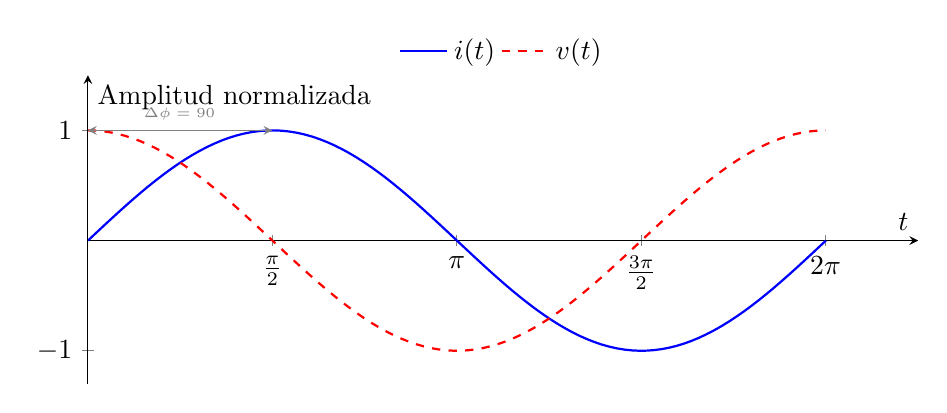
\begin{tikzpicture}
        \begin{axis}[
            width=\linewidth, height=5.5cm,
            xlabel={$t$}, ylabel={Amplitud normalizada},
            xmin=0, xmax=2*pi+pi/4,
            ymin=-1.3, ymax=1.5,
            axis lines=middle,
            xtick={0, 1.57, 3.14, 4.71, 6.28},
            xticklabels={0, $\frac{\pi}{2}$, $\pi$, $\frac{3\pi}{2}$, $2\pi$},
            ytick={-1, 1},
            legend style={at={(0.5,1)}, anchor=south, legend columns=-1, draw=none}
        ]
            % Corriente i(t) - Azul
            \addplot[thick, blue, domain=0:2*pi, samples=100] {sin(deg(x))};
            \addlegendentry{$i(t)$}

            % Tensión v(t) - Roja (Adelantada 90 grados para un inductor)
            \addplot[thick, red, dashed, domain=0:2*pi, samples=100] {cos(deg(x))};
            \addlegendentry{$v(t)$}

            % Indicación del adelanto (Lead)
            \draw[<->, >=stealth, gray] (axis cs:0, 1) -- (axis cs:1.57, 1);
            \node[gray, font=\tiny, anchor=south] at (axis cs:0.78, 1) {$\Delta \phi = \qty{90}{\degree}$};
        \end{axis}
    \end{tikzpicture}
    \caption[Representación temporal del desfase en un inductor ideal.]{Representación temporal del desfase en un inductor ideal. La curva de tensión (roja) alcanza su valor máximo un cuarto de ciclo antes que la de corriente (azul).}\label{fig:fase_temporal}
\end{marginfigure}

\paragraph{El Inductor: La tensión adelanta a la corriente}
Físicamente, un inductor se opone a las variaciones bruscas de la intensidad de corriente debido a la Ley de Lenz. La corriente tarda un tiempo en establecerse tras aplicar una diferencia de potencial. 

Matemáticamente, la relación es diferencial: $v(t) = L \frac{di(t)}{dt}$. Si la corriente es una señal senoidal $i(t) = I_0 \sin(\omega t)$, la tensión resultante es:
\begin{equation}
    v(t) = L \cdot \omega I_0 \cos(\omega t) = V_0 \sin(\omega t + \qty{90}{\degree})
\end{equation}


\paragraph{El Condensador: La corriente adelanta a la tensión}
En un condensador, la tensión entre sus placas no puede cambiar instantáneamente; requiere el flujo previo de portadores de carga (corriente). Por tanto, la corriente debe fluir antes de que se observe un aumento en la tensión.

La relación es $i(t) = C \frac{dv(t)}{dt}$. Si aplicamos una tensión $v(t) = V_0 \sin(\omega t)$, la corriente es:
\begin{equation}
    i(t) = C \cdot \omega V_0 \cos(\omega t) = I_0 \sin(\omega t + \qty{90}{\degree})
\end{equation}

\paragraph{Implicaciones en Instrumentación:}
Para un ingeniero electrónico, el concepto de adelanto o retardo se traduce en la posición del vector en el plano complejo:
\begin{itemize}
    \item Un adelanto de $\qty{90}{\degree}$ sitúa el fasor en el eje imaginario positivo ($+j$).
    \item Un retardo de $\qty{90}{\degree}$ lo sitúa en el eje imaginario negativo ($-j$).
\end{itemize}

En los capítulos siguientes veremos que el \emph{LVDT} utiliza precisamente este desfase para determinar la dirección del movimiento: si el núcleo se desplaza hacia un lado, la señal está en fase ($\phi=\qty{0}{\degree}$); si se desplaza hacia el otro, se invierte por completo ($\phi=\qty{180}{\degree}$).

% \begin{marginfigure}
%     \centering
%     \shorthandoff{>}
%     \begin{tikzpicture}[american, scale=1]
%         % --- DIBUJO (a): CAPACITIVO ---
%         \begin{scope}
%             % Placas
%             \draw[ultra thick, fill=gray!20] (0,0.8) rectangle (2,1);
%             \draw[ultra thick, fill=gray!20] (0,0) rectangle (2,0.2);
%             % Líneas de campo E
%             \foreach \x in {0.2,0.6,...,2.2} {
%                 \draw[blue, -stealth, thin] (\x, 0.78) -- (\x, 0.22);
%             }
%             \node[blue, font=\tiny] at (2.3, 0.4) {$\vec{E}$};
%             \node at (1, -0.6) {\textbf{(a) Almacenamiento en } $\vec{E}$};
%         \end{scope}

%         % --- DIBUJO (b): INDUCTIVO ---
%         \begin{scope}[yshift=-3.8cm]
%             \draw (0,0.5) to[L, l=$L$, color=red!70!black] (2,0.5);
%             % Líneas de campo B (elipses)
%             \draw[red!70!black, dashed, thin] (1,0.5) ellipse (1.2cm and 0.5cm);
%             \draw[red!70!black, dashed, thin] (1,0.5) ellipse (0.8cm and 0.3cm);
%             \node[red!70!black, font=\tiny] at (2.2, 1.1) {$\vec{B}$};
%             \node at (1, -0.6) {\textbf{(b) Almacenamiento en } $\vec{B}$};
%         \end{scope}
%     \end{tikzpicture}
%     \caption{Interacción con los campos en sensores reactivos. La variación de la capacidad depende de la permitividad y la geometría de las placas, mientras que la inductancia depende de la permeabilidad del núcleo y la configuración del devanado.}\label{fig:fundamentos_reactivos}
% \end{marginfigure}

\subsection{Figuras de Mérito: El Factor de Calidad ($Q$)}
En un diseño de ingeniería real, los sensores reactivos no son puros. Presentan pérdidas debidas a la resistencia del conductor (en inductores) o a las corrientes de fuga y polarización del dieléctrico (en condensadores). Para caracterizar la eficiencia del sensor se emplea el \emph{Factor de Calidad ($Q$)}:

\begin{equation}\label{eq:factor_q}
    Q = \frac{\text{Energía almacenada}}{\text{Energía disipada por ciclo}}
\end{equation}

Para modelos con resistencia serie ($R_s$):
\begin{itemize}
    \item \emph{Inductor}: $Q_L = \dfrac{\omega L}{R_s}$ (Aumenta con la frecuencia).
    \item \emph{Condensador}: $Q_C = \dfrac{1}{\omega C R_s}$ (Disminuye con la frecuencia).
\end{itemize}

\marginnote{\textbf{Consideración de Diseño:} Un sensor con un $Q$ bajo se comporta de forma cuasi-resistiva, perdiendo la ventaja de la inmunidad al ruido térmico y dificultando el diseño de circuitos resonantes estables. En 4º curso se asume que un sensor de instrumentación de alta gama debe operar en zonas donde $Q > 50$.
}

\subsection{Ventajas del Uso de Reactancias}
El salto tecnológica de la medida resistiva a la reactiva ofrece ventajas críticas:
\begin{enumerate}
    \item \emph{Ausencia de Ruido Térmico}: Puesto que el ruido de Johnson-Nyquist es proporcional a la parte real de la impedancia ($R$), un sensor puramente reactivo es idealmente silencioso.
    \item \emph{Sensibilidad Estática}: Muchos materiales dieléctricos (aire, cuarzo) son extremadamente estables frente a variaciones de temperatura comparados con los semiconductores de una NTC.
    \item \emph{Bajo Consumo}: No requieren circular una corriente de excitación constante para mantener la información; la energía se devuelve a la fuente en cada semiciclo.
\end{enumerate}

\section{Sensores Capacitivos}\label{sec:capacitivos}

Los sensores capacitivos convierten cambios de una magnitud física en cambios de la capacidad de un condensador. Partiendo del modelo de placas paralelas:
\begin{equation}\label{eq:capacidad_placas}
    C = \epsilon_0 \epsilon_r \frac{A}{d}
\end{equation}
donde $\epsilon_0$ es la permitividad del vacío, $\epsilon_r$ la permitividad relativa del dieléctrico, $A$ el área efectiva de las placas y $d$ la distancia de separación.

\subsection{Principios de Funcionamiento}
% Variación de distancia (d), área (A) y constante dieléctrica (epsilon).

Los sensores capacitivos basan su funcionamiento en la modificación de uno o más parámetros de la ecuación fundamental del condensador de placas paralelas:

\paragraph{Variación de la Distancia ($d$):}
Es el método más común para medir desplazamientos microscópicos o presiones. Si una placa se desplaza una distancia $x$ respecto a la posición inicial $d_0$, la capacidad es:
\begin{equation}
    C(x) = \frac{\epsilon A}{d_0 - x} = C_0 \frac{1}{1 - x/d_0}
\end{equation}
La respuesta es \emph{no lineal} (hiperbólica). Sin embargo, su sensibilidad ($S = dC/dx$) aumenta a medida que las placas se aproximan, lo que permite detectar variaciones del orden de los nanómetros. Para mantener la linealidad, se suele restringir su uso a desplazamientos $x \ll d_0$ o se emplean configuraciones diferenciales.

\paragraph{Variación del Área ($A$):}
Se obtiene mediante el desplazamiento lateral de una placa sobre la otra. Si las placas tienen un ancho $w$ y el solapamiento inicial es $L$, un desplazamiento $x$ resulta en:
\begin{equation}
    C(x) = \frac{\epsilon \cdot w \cdot (L - x)}{d} = C_0 \left( 1 - \frac{x}{L} \right)
\end{equation}
A diferencia del método anterior, la relación es \emph{intrínsecamente lineal}. Es la configuración preferida para sensores de desplazamiento lineal de largo recorrido o sensores de rotación angular (usando placas semicirculares).

\paragraph{Variación del Dieléctrico ($\epsilon_r$):}
El sensor consta de placas fijas, y la magnitud física (como el nivel de un líquido o la humedad ambiental) altera la permitividad efectiva del medio.
\begin{equation}
    C_{total} = C_{fixed} + \Delta C(\epsilon_r)
\end{equation}
Es el principio utilizado en la medida de humedad (el polímero absorbe agua, variando su $\epsilon_r$) y en la monitorización de calidad de aceites o nivel de combustibles.

\begin{marginfigure}[-15em]
    \centering
    \shorthandoff{>}
    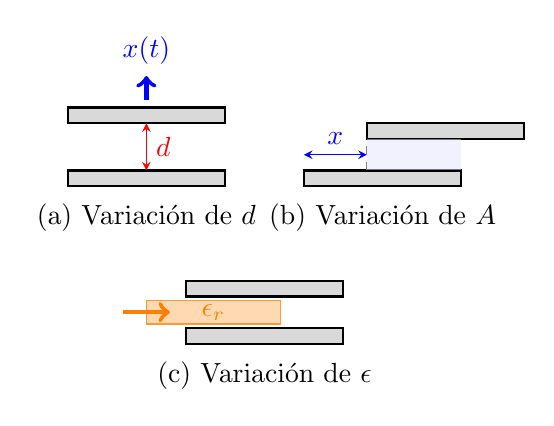
\begin{tikzpicture}[scale=1]
        % Estilo de las placas
        \tikzset{placa/.style={fill=gray!30, draw=black, thick}}
        
        % --- MODO A: VARIACIÓN DE DISTANCIA ---
        \begin{scope}[xshift=-1.5cm]
            \draw[placa] (0,0.8) rectangle (2,1);
            \draw[placa] (0,0) rectangle (2,0.2);
            \draw[<->, >=stealth, red] (1, 0.2) -- (1, 0.8) node[midway, right] {$d$};
            \draw[->, ultra thick, blue] (1, 1.1) -- (1, 1.4) node[above] {$x(t)$};
            \node at (1, -0.4) {(a) Variación de $d$};
        \end{scope}

        % --- MODO B: VARIACIÓN DE ÁREA ---
        \begin{scope}[xshift=1.5cm]
            \draw[placa] (0.8,0.6) rectangle (2.8,0.8);
            \draw[placa] (0,0) rectangle (2,0.2);
            \draw[dashed, gray] (0.8,0.2) -- (0.8,0.6);
            \draw[<->, >=stealth, blue] (0, 0.4) -- (0.8, 0.4) node[midway, above] {$x$};
            \fill[blue!10, opacity=0.5] (0.8, 0.2) rectangle (2, 0.6);
            \node at (1, -0.4) {(b) Variación de $A$};
        \end{scope}

        % --- MODO C: VARIACIÓN DE DIELÉCTRICO ---
        \begin{scope}[yshift=-2cm]
            \draw[placa] (0,0.6) rectangle (2,0.8);
            \draw[placa] (0,0) rectangle (2,0.2);
            % Dieléctrico entrando
            \draw[fill=orange!30, draw=orange!80] (-0.5, 0.25) rectangle (1.2, 0.55);
            \draw[->, ultra thick, orange] (-0.8, 0.4) -- (-0.2, 0.4);
            \node[orange] at (0.35, 0.4) {$\epsilon_r$};
            \node at (1, -0.4) {(c) Variación de $\epsilon$};
        \end{scope}
    \end{tikzpicture}
    \caption[Métodos de transducción en sensores capacitivos.]{Métodos de transducción en sensores capacitivos. La elección del modo de operación define la sensibilidad y el rango dinámico del sensor.}\label{fig:modos_capacitivos}
\end{marginfigure}


\subsection{Modelos de Sensibilidad y Linealidad}
% Modelos de sensibilidad y linealidad.

El diseño de un sistema de instrumentación capacitivo exige evaluar el compromiso entre la \emph{sensibilidad absoluta} ($S = dC/dx$) y el \emph{error de no linealidad}. Dependiendo del parámetro geométrico que se modifique, el comportamiento del sensor varía drásticamente, como se resume en la Tabla~\ref{tab:sensibilidad_capacitiva}.

\begin{table}[ht]
    \centering
    \setlength{\tabcolsep}{3pt} % Reducimos el espacio entre columnas
    \small
    \begin{tabularx}{\linewidth}{l c c X}
        \toprule
        \textbf{Modo} & \textbf{Ecuación $C(x)$} & \textbf{Sensibilidad ($S$)} & \textbf{Linealidad} \\
        \midrule
        \emph{Área} ($A$) & $C_0 (1 - \dfrac{x}{L})$ & $-\dfrac{\epsilon w}{d}$ (Constante) & Excelente (Lineal) \\
        \midrule
        \emph{Distancia ($d$)} & $\dfrac{C_0}{1 - x/d_0}$ & $\dfrac{C_0 / d_0}{(1 - x/d_0)^2}$ (Variable) & Pobre (Hiperbólica) \\
        \bottomrule
    \end{tabularx}
    \caption{Comparativa de modelos de sensibilidad. La variación de distancia ofrece una sensibilidad mucho mayor a costa de una respuesta no lineal.}\label{tab:sensibilidad_capacitiva}
\end{table}

\begin{marginfigure}
    \centering
    \shorthandoff{>}
    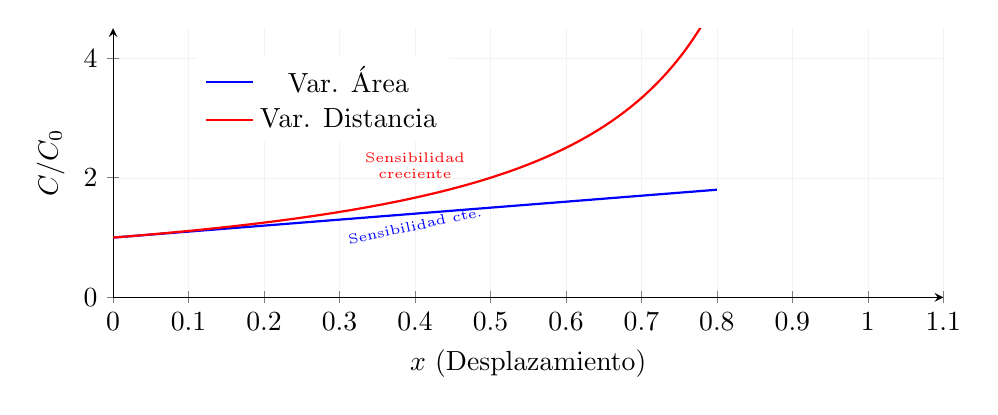
\begin{tikzpicture}
        \begin{axis}[
            width=\linewidth, height=5cm,
            xlabel={$x$ (Desplazamiento)}, ylabel={$C/C_0$},
            xmin=0, xmax=1.1, ymin=0, ymax=4.5,
            axis lines=left, grid=both,
            grid style={line width=.1pt, draw=gray!10},
            %font=\scriptsize,
            legend style={at={(0.1,0.9)}, anchor=north west, draw=none}
        ]
            % Variación de Área (Lineal)
            \addplot[thick, blue, domain=0:0.8] {1 + x};
            \addlegendentry{Var. Área}

            % Variación de Distancia (Hiperbólica)
            \addplot[thick, red, domain=0:0.8, samples=100] {1 / (1 - x)};
            \addlegendentry{Var. Distancia}
            
            \node[red, font=\tiny, align=center] at (axis cs:0.4, 2.2) {Sensibilidad\\creciente};
            \node[blue, font=\tiny, rotate=12] at (axis cs:0.4, 1.2) {Sensibilidad cte.};
        \end{axis}
    \end{tikzpicture}
    \caption[Comparativa de respuesta variación Área y Distancia.]{Comparativa de respuesta. El sensor de distancia es ideal para desplazamientos ínfimos (nanómetros), mientras que el de área es preferible para rangos mayores.}\label{fig:curvas_sensibilidad}
\end{marginfigure}

\paragraph{Linealización mediante Configuraciones Diferenciales:}

En ingeniería de precisión, el problema de la no linealidad hiperbólica de los sensores de distancia se resuelve mediante el uso de un \emph{condensador diferencial} o configuración \textit{Push-Pull}. Este sistema consta de tres placas: dos fijas y una central móvil.

Si la placa central se desplaza una distancia $x$ desde el centro equilibrado ($d_0$), las capacidades resultantes son:
\begin{equation}
    C_1 = \frac{\epsilon A}{d_0 - x} \quad ; \quad C_2 = \frac{\epsilon A}{d_0 + x}
\end{equation}

Al procesar la señal de forma diferencial ($\Delta C = C_1 - C_2$), la expresión resultante mejora significativamente la linealidad:
\begin{equation}
    \Delta C = C_0 \left( \frac{1}{1-x/d_0} - \frac{1}{1+x/d_0} \right) = C_0 \left( \frac{2x/d_0}{1 - (x/d_0)^2} \right)
\end{equation}

Para desplazamientos pequeños ($x \ll d_0$), el término cuadrático del denominador se desprecia, obteniendo una respuesta lineal:
\begin{equation}
    \Delta C \approx 2 C_0 \frac{x}{d_0}
\end{equation}

\marginnote{\textbf{Ventaja del diferencial:} 
    Además de duplicar la sensibilidad ($2C_0/d_0$), esta topología cancela por \textit{modo común} los errores debidos a variaciones térmicas del dieléctrico, ya que afectan a $C_1$ y $C_2$ por igual y se restan en la etapa de acondicionamiento.
}

\begin{marginfigure}
    \centering
    \shorthandoff{>}
    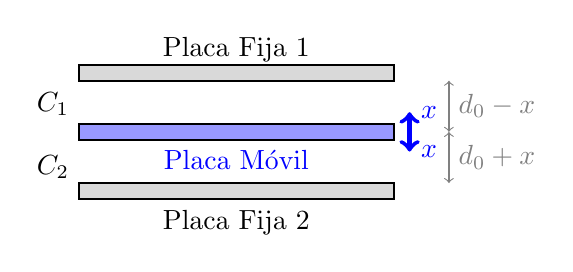
\begin{tikzpicture}[scale=1]
        % Placas fijas
        \draw[fill=gray!30, thick] (0,1.5) rectangle (4,1.7);
        \draw[fill=gray!30, thick] (0,0) rectangle (4,0.2);
        
        % Placa móvil central
        \draw[fill=blue!40, thick] (0,0.75) rectangle (4,0.95);
        \draw[->, ultra thick, blue] (4.2, 0.85) -- (4.2, 1.1) node[right] {$x$};
        \draw[->, ultra thick, blue] (4.2, 0.85) -- (4.2, 0.6) node[right] {$x$};
        
        % Etiquetas
        \node at (2, 1.9) {Placa Fija 1};
        \node at (2, -0.3) {Placa Fija 2};
        \node[blue] at (2, 0.5) {Placa Móvil};
        
        % Dimensiones d0
        \draw[<->, gray] (4.7, 0.2) -- (4.7, 0.85) node[midway, right] {$d_0+x$};
        \draw[<->, gray] (4.7, 0.85) -- (4.7, 1.5) node[midway, right] {$d_0-x$};
        
        % Capacidades
        \node[left] at (0, 1.2) {$C_1$};
        \node[left] at (0, 0.4) {$C_2$};
    \end{tikzpicture}
    \caption[Esquema de un sensor capacitivo diferencial.]{Esquema de un sensor capacitivo diferencial. Es la arquitectura base de los acelerómetros MEMS y sensores de presión de alta gama.}\label{fig:sensor_diferencial}
\end{marginfigure}

\paragraph{Conclusión para el Diseño}
Para un ingeniero electrónico, la elección depende del rango dinámico requerido:
\begin{enumerate}
    \item \emph{Alta Linealidad}: Usar variación de área o configuraciones diferenciales en rango central.
    \item \emph{Alta Sensibilidad}: Usar variación de distancia con huecos ($d_0$) muy pequeños, asumiendo la necesidad de compensación por software de la no linealidad.
\end{enumerate}

\subsection{Problemas de Implementación: Capacidades Parásitas}
% Introducción al blindaje y técnicas de guarda (Guarding).

La medida de la capacidad plantea un reto tecnológico mayor que la de la resistencia. Mientras que los sensores resistivos suelen tener valores de \unit{k\Omega}, los sensores capacitivos presentan valores extremadamente bajos, típicamente en el rango de los \unit{pF} ($10^{-12}$ F) o incluso \unit{fF} ($10^{-15}$ F).

\paragraph{El Efecto del Cable de Conexión} El principal enemigo de un sensor capacitivo es el cable que lo une a la electrónica. Un cable coaxial estándar presenta una capacidad parásita de entre \qtyrange{50}{100}{pF/m}. 

Si intentamos medir un sensor de \unit{1}{pF} mediante un cable de \unit{1}{m}, la capacidad del cable es \emph{100 veces superior} a la del sensor, actuando como un condensador en paralelo que enmascara la señal y degrada la sensibilidad. 
%
\begin{marginfigure}[0em]
    \centering
    \shorthandoff{>}
    \begin{tikzpicture}[american, scale=1]
        %\ctikzset{resistors/scale=0.6, capacitors/scale=0.6}
        % Sensor
        \draw (0,2) to[C, l_=$C_s$] (0,0) node[ground]{};
        % Cable coaxial (modelo)
        \draw (0,2) -- (1,2) coordinate(A);
        \draw (1,2) to[C, l=$C_p$ (cable)] (1,0) node[ground]{};
        \draw (1,2) -- (2,2) node[ocirc]{} node[right]{Electrónica};
        
        \node[blue] at (0, 2.3) {SENSOR};
        \node[red] at (1, 0.3) {PARÁSITA};
    \end{tikzpicture}
    \caption[Efecto de la capacidad parásita del cable.]{Efecto de la capacidad parásita del cable. $C_p$ aparece en paralelo con el sensor, sumándose a la medida y reduciendo drásticamente la variación relativa $\Delta C/C_{total}$.}\label{fig:cable_parasito}
\end{marginfigure}
%
Dos condensadores en paralelo, uno de \unit{1}{pF} y otro de \unit{100}{pF}, representan un \emph{sensor de baja capacidad degradado por la capacidad parásita} de un cable de conexión de longitud moderada (aprox. \unit{1}{m}). 

\paragraph{Análisis de la Degradación de Sensibilidad}
Para un ingeniero, el problema no es que la capacidad total sea mayor, sino que la \emph{sensibilidad relativa} del sistema se desploma. Consideremos que el sensor de \unit{1}{pF} experimenta una variación del \unit{10}{\%} ante un estímulo físico ($\Delta C_s = \unit{0,1}{pF}$).

\begin{enumerate}
    \item \emph{Caso Ideal (Sin cable)}: 
    La variación relativa que detecta la electrónica es:
    \[ \frac{\Delta C}{C} = \frac{\unit{0,1}{pF}}{\unit{1}{pF}} = \mathbf{\unit{10}{\%}} \]
    
    \item \emph{Caso Real (Con cable de \unit{100}{pF})}:
    La capacidad total es $C_T = C_s + C_p = \unit{101}{pF}$. La variación relativa que detecta la electrónica ahora es:
    \[ \frac{\Delta C}{C_T} = \frac{\unit{0,1}{pF}}{\unit{101}{pF}} \approx \mathbf{\unit{0,1}{\%}} \]
\end{enumerate}

\marginnote{\textbf{Solución a la atenuación de la sensibilidad:}
        La presencia de la capacidad parásita ha \emph{atenuado la sensibilidad en un factor de 100}. Para recuperar la medida, necesitaríamos un ADC con 7 bits adicionales de resolución o un amplificador con una ganancia masiva que, inevitablemente, amplificaría también el ruido.
}

\begin{marginfigure}
    \centering
    \shorthandoff{>}
    \begin{tikzpicture}[american, scale=1]
        \ctikzset{capacitors/scale=0.7}
        % Nodo de entrada
        \draw (0,2) -- (3,2);
        % Sensor
        \draw (0.5,2) to[C, l=$C_s$, v=$\Delta C$] (0.5,0) node[ground]{};
        % Parásita
        \draw (2.5,2) to[C, l=$C_p$] (2.5,0) node[ground]{};
        
        \node[blue] at (0.5, 2.3) {\unit{1}{pF}};
        \node[red] at (2.5, 2.3) {\unit{100}{pF}};
        
        % Flecha de suma
        \draw[thick, ->, >=stealth] (3.3,1) -- (3.6,1) node[right] {$C_{total} = \unit{101}{pF}$};
    \end{tikzpicture}
    \caption{Modelo equivalente del sensor y el cable. La gran magnitud de $C_p$ enmascara los pequeños cambios de $C_s$.}\label{fig:paralelo_capacitivo}
\end{marginfigure}

\paragraph{Estrategias de Mitigación}
Ante este escenario, el ingeniero de diseño tiene tres opciones:
\begin{itemize}
    \item \emph{Electrónica de proximidad}: Colocar el convertidor $C/V$ o el microcontrolador justo al lado del sensor (minimizando la longitud del cable).
    \item \emph{Guarda Activa}: Utilizar la técnica de \textit{guarding} analizada anteriormente para anular eléctricamente el efecto de $C_p$.
    \item \emph{Medida en Frecuencia}: Integrar el condensador en un oscilador, donde la frecuencia de salida $f \propto 1/\sqrt{C}$ suele ser más robusta frente a ruidos de amplitud, aunque la no linealidad persiste.
\end{itemize}


\paragraph{Blindaje Activo o Técnica de Guarda (\textit{Guarding})}
Para eliminar el efecto de $C_p$, no basta con blindar el cable (conectando la malla a masa); esto solo protegería frente a ruido externo, pero mantendría la capacidad parásita. La solución profesional es la \emph{Guarda Activa}.

\marginnote{\textbf{Principio de la Guarda:} 
    Si mantenemos los dos conductores de un condensador al \textbf{mismo potencial} ($V_1 = V_2$), la diferencia de tensión es nula. Según $Q = C \cdot \Delta V$, la carga acumulada es cero y, por tanto, no circula corriente a través de esa capacidad. \textit{Físicamente, la capacidad parásita sigue ahí, pero el circuito no la ``ve''}.
}

En esta técnica, se utiliza un seguidor de tensión (buffer) para alimentar el blindaje interno con exactamente la misma tensión que lleva el hilo de señal.

% \begin{marginfigure}
%     \centering
%     \shorthandoff{>}
%     \ctikzset{amplifiers/fill=blue!5, capacitors/scale=0.6}
%     %\usetikzlibrary{circuits.ee.IEC}
%     \begin{tikzpicture}[american, scale=1] 
%         % Sensor
%         \draw (0,2) to[C, l=$C_s$] (0,0) node[ground]{};
        
%         % Seguidor de tensión (Guarda)
%         \draw (2,1) node[op amp, scale=0.6] (opamp) {};
%         \draw (0,2) -- (1,2) |- (opamp.+);
%         \draw (opamp.out) -- ++(0,0.5) -| (opamp.-);
        
%         % Conexión a la guarda
%         \draw (opamp.out) -- ++(0.5,0) coordinate(G);
        
%         % Representación del cable triaxial o guarda
%         \draw[thick, gray] (0.8, 2.2) rectangle (2.8, 1.8);
%         \node[gray, font=\tiny] at (1.8, 2.4) {GUARDA};
%         \draw (G) |- (1.8, 1.8);
        
%         % Capacidades eliminadas
%         \draw[red, dashed] (1.5, 2) to[C, l=$C_p$, color=red] (1.5, 1.8);
        
%     \end{tikzpicture}
%     \caption{Esquema de guarda activa. El amplificador asegura que el potencial de la guarda sea idéntico al de la señal, anulando la corriente a través de $C_p$.}\label{fig:guarda_activa}
% \end{marginfigure}

\begin{marginfigure}
    \centering
    \shorthandoff{>}
    \begin{tikzpicture}[american, scale=1]
        % Ajustes de componentes
        \ctikzset{resistors/scale=0.6, capacitors/scale=0.6, amplifiers/fill=blue!5}

        % --- LÍNEA DE SEÑAL PRINCIPAL ---
        \draw (0,0) node[ground]{} 
              to[C, l=$C_s$] (0,2.5)      % Sensor
              to[short] (0.8,2.5)     % Punto de toma para el buffer
              -- (5,2.5) node[ocirc, scale=0.6] {} node[above] {Acond.};

        % --- EL SEGUIDOR DE TENSIÓN (BUFFER) ---
        % Lo situamos debajo para que no estorbe
        \draw (1.75,1) node[op amp, scale=0.7] (OA) {};
        
        % Conexión de entrada (+) al cable de señal
        \draw (0.5,2.5) node[circ,scale=0.6]{} |- (OA.+);
        
        % Realimentación unitaria (Salida a entrada -)
        \draw (OA.out)node[circ,scale=0.6]{} -- ++(0,0.95) -| (OA.-);
        \node[blue!50, font=\tiny\bfseries] at (3, .3) {BUFFER (Seguidor de tensión)};

        % --- LA GUARDA (CABLE BLINDADO) ---
        % Dibujamos la guarda como una caja gris que envuelve el cable
        \draw[thick, gray!80] (1.5, 2.1) rectangle (4.5, 2.9);
        \node[gray!80, font=\tiny\bfseries] at (3, 3.1) {GUARDA (Malla)};

        % Conexión de la salida del buffer a la guarda
        \draw (OA.out) -- ++(0.4,0) |- (2.98, 2.1)node[circ,scale=0.6]{};

        % --- CAPACIDAD PARÁSITA ELIMINADA ---
        % Se dibuja entre el hilo interno (2.5) y la malla (2.1)
        \draw[red, dashed, thick] (3.8, 2.5) to[C, l=$C_p$] (3.8, 2.1);
        
        % Nota aclaratoria
        \node[red, font=\tiny, align=center] at (4.3, 1.7) {$V_{sig} \approx V_{guard}$  $\implies I_{Cp} \approx 0$};

    \end{tikzpicture}
    \caption{Esquema de guarda activa. El buffer de ganancia unidad asegura que la malla del cable esté al mismo potencial que el hilo de señal ($V_{sig} \approx V_{guard}$), eliminando la corriente a través de $C_p$. Al no haber diferencia de tensión entre los terminales de $C_p$, esta capacidad no se carga ni descarga, eliminando su efecto en la medida del sensor.}\label{fig:guarda_activa}
\end{marginfigure}

\paragraph{Implementación en PCB: El Anillo de Guarda}
En el diseño de circuitos impresos (PCB), las corrientes de fuga por la superficie de la placa y las capacidades entre pistas también falsean la medida. Para evitarlo, se rodea la pista de alta impedancia del sensor con un \emph{anillo de guarda} conectado al mismo potencial.

\begin{marginfigure}
    \centering
    \shorthandoff{>}
    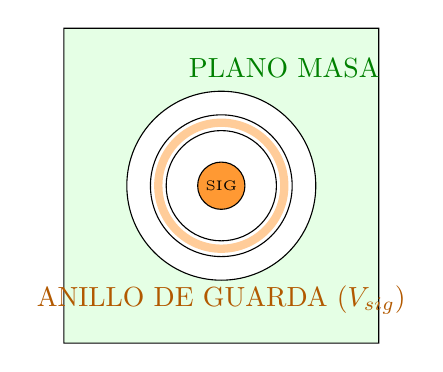
\begin{tikzpicture}[scale=1]
        % Pista de señal
        \draw[fill=orange!80, draw=black] (0,0) circle (0.3);
        \node[font=\tiny] at (0,0) {SIG};
        
        % Anillo de guarda
        \draw[line width=3pt, orange!40] (0,0) circle (0.8);
        \draw[draw=black, thin] (0,0) circle (0.7);
        \draw[draw=black, thin] (0,0) circle (0.9);
        
        
        % Masa exterior
        \draw[fill=green!10, even odd rule] (-2,-2) rectangle (2,2) (0,0) circle (1.2);
        % Textos
        \node[green!50!black] at (0.8, 1.5) {PLANO MASA};
        \node[orange!70!black] at (0,-1.45) {ANILLO DE GUARDA ($V_{sig}$)};

    \end{tikzpicture}
    \caption[Diseño de un anillo de guarda en PCB.]{Diseño de un anillo de guarda en PCB. El anillo actúa como una barrera de potencial que intercepta corrientes de fuga y neutraliza capacidades parásitas laterales.}\label{fig:anillo_guarda}
\end{marginfigure}

\marginnote{\textbf{Aplicación Anillo de Guarda}: Esta técnica es obligatoria en sensores de \textbf{humedad capacitivos} y en \textbf{acelerómetros MEMS}, donde las variaciones de señal son tan pequeñas que el simple aire entre pistas de la PCB podría actuar como una carga capacitiva inaceptable.
}
\subsection{Aplicaciones Típicas de los Sensores Capacitivos}\label{sec:aplicaciones_capacitivas}

La versatilidad de la transducción capacitiva permite su uso en una amplia gama de magnitudes físicas, aprovechando la ausencia de contacto mecánico y su alta resolución intrínseca.

\paragraph{1. Medida de Nivel de Líquidos}
Se basa en la variación de la permitividad efectiva ($\epsilon_r$) entre dos electrodos fijos (normalmente cilindros concéntricos o placas paralelas) sumergidos en un tanque como se muestra en la figura \ref{fig:nivel_capacitivo}. 

\begin{marginfigure}
    \centering
    \shorthandoff{>}
    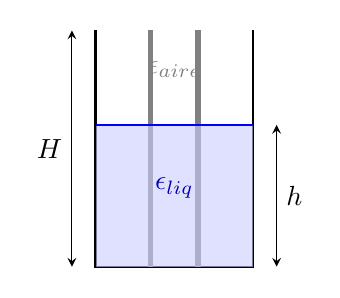
\begin{tikzpicture}[scale=1]
        % Tanque
        \draw[thick] (0,3) -- (0,0) -- (2,0) -- (2,3);
        % Electrodos (Capacitor)
        \draw[line width=2pt, gray] (0.7, 3) -- (0.7, 0);
        \draw[line width=2pt, gray] (1.3, 3) -- (1.3, 0);
        
        % Líquido
        \fill[blue!20, opacity=0.6] (0,0) rectangle (2,1.8);
        \draw[blue, thick] (0,1.8) -- (2,1.8);
        
        % Cotas
        \draw[<->, >=stealth] (2.3, 0) -- (2.3, 1.8) node[midway, right] {$h$};
        \draw[<->, >=stealth] (-0.3, 0) -- (-0.3, 3) node[midway, left] {$H$};
        
        \node[blue!70!black] at (1, 1) {$\epsilon_{liq}$};
        \node[gray] at (1, 2.5) {$\epsilon_{aire}$};
    \end{tikzpicture}
    \caption[Medida de nivel capacitiva.]{Medida de nivel capacitiva. El líquido actúa como un dieléctrico variable que rellena el espacio entre las placas a medida que sube el nivel $h$.}\label{fig:nivel_capacitivo}
\end{marginfigure}

Si el líquido es no conductor (dieléctrico), la capacidad total puede modelarse como la suma de dos condensadores en paralelo: uno con aire y otro sumergido. La capacidad resultante es lineal respecto a la altura $h$:
\begin{equation}
    C(h) = \frac{\epsilon_0 \cdot w}{d} \left[ h \cdot \epsilon_{liq} + (H - h) \cdot \epsilon_{aire} \right]
\end{equation}
donde $w$ es el ancho de las placas y $d$ la distancia entre ellas, $H$ la altura total del tanque y $h$ la altura del líquido. La variación de capacidad es proporcional a la altura del líquido, permitiendo una medida precisa del nivel.

\paragraph{2. Sensores de Humedad Relativa}
Utilizan un polímero higroscópico como dieléctrico. Este material tiene la propiedad de absorber moléculas de agua del aire, lo que altera su permitividad relativa ($\epsilon_r$) de forma proporcional a la humedad ambiente. 

\marginnote{\textbf{Dato técnico:} El agua pura tiene una $\epsilon_r \approx 80$, mientras que los polímeros secos tienen $\epsilon_r \approx 3$. Por ello, incluso una pequeña absorción de humedad provoca cambios de capacidad detectables con gran precisión.
}

\paragraph{3. Pantallas Táctiles y Sensores de Proximidad}
En las pantallas capacitivas, el dedo humano actúa como una ``tercera placa'' o un camino a masa como se esquematiza en la Figura \ref{fig:touch_capacitivo}. Al acercar el dedo, se distorsiona el campo eléctrico proyectado, creando una capacidad parásita que la electrónica localiza con alta resolución espacial.

\begin{marginfigure}
    \centering
    \shorthandoff{>}
    \begin{tikzpicture}[scale=1]
        % Panel de cristal
        \draw[fill=cyan!10] (0,0.5) rectangle (5,1);
        \node at (2.5, 0.8) {Cristal / Dieléctrico};
        
        % Electrodos
        \draw[ultra thick, orange] (0.5, 0.4) -- (2, 0.4);
        \draw[ultra thick, orange] (3, 0.4) -- (4.5, 0.4);
        \node[orange] at (1.25, 0.2) {Electrodo X};
        \node[orange] at (3.75, 0.2) {Electrodo Y};
        
        % Dedo (Esquema)
        \draw[fill=orange!20, rounded corners=5pt] (2.2, 3) -- (2.2, 1.7) -- (2.8, 1.7) -- (2.8, 3);
        \node at (2.5, 3.2) {Dedo (GND)};
        
        % Capacidad inducida
        \draw[red, dashed, thick] (2.5, 1.7) to[C, l=$C_{touch}$] (2.5, 0.7);
    \end{tikzpicture}
    \caption{Principio del \textit{touchscreen} capacitivo. El cuerpo humano altera el campo eléctrico proyectado por la matriz de electrodos.}\label{fig:touch_capacitivo}
\end{marginfigure}

\paragraph{4. Acelerómetros MEMS y Sensores de Presión}
En la microelectrónica de consumo (\textit{smartphones}), los acelerómetros son estructuras de silicio donde la aceleración desplaza una masa móvil, variando la distancia $d$ entre micro-placas. Estos sensores miden variaciones en el rango de los \unit{fF} (femtofaradios).

\marginnote{\textbf{Ventaja en MEMS:} La transducción capacitiva no requiere circular corriente constante por el sensor (a diferencia de las galgas), lo que reduce drásticamente el consumo de batería en dispositivos móviles.
}

\paragraph{5. Micrófonos de Condensador}
Consisten en un diafragma elástico que vibra con las ondas sonoras frente a una placa fija. El cambio en la distancia $d$ modula la capacidad a la frecuencia del sonido. Requieren una tensión de polarización (típicamente \unit{48}{V}, o \textit{Phantom Power}) para convertir el movimiento en una señal eléctrica medible.

% Sensores de proximidad, nivel de líquidos y humedad.

% ============================================================
%  SECCIÓN 4.3 — SENSORES INDUCTIVOS Y ELECTROMAGNÉTICOS
%  Para insertar en capitulo4.tex con \input{sec_inductivos}
%  Requiere: circuitikz, pgfplots, tikz, siunitx, booktabs,
%            tabularx, amsmath  (todos ya cargados en main.tex)
% ============================================================

\section{Sensores Inductivos y Electromagnéticos}\label{sec:inductivos}

Los sensores inductivos explotan la relación entre el movimiento mecánico y el campo magnético. Su principio de operación descansa en la \emph{Ley de Faraday}: cualquier cambio en el flujo magnético $\Phi$ que atraviesa un bobinado de $N$ espiras induce una fuerza electromotriz (f.e.m.):

\begin{equation}
  \mathcal{E} = -N \frac{d\Phi}{dt} = -N \frac{d(B \cdot A)}{dt}
\end{equation}
donde $B$ es la densidad de flujo magnético y $A$ el área del circuito magnético. Al variar $B$ o $A$ mediante el movimiento de una armadura, se genera una señal eléctrica proporcional a la velocidad del cambio.

A diferencia de los sensores resistivos o capacitivos, los sensores inductivos presentan \emph{inmunidad intrínseca al ruido eléctrico} (son insensibles a campos eléctricos externos) y toleran entornos industriales con vibraciones, suciedad y alta temperatura, razón por la que dominan en automoción, aeronáutica y manufactura pesada.

% -----------------------------------------------------------
\subsection{Sensores de Inductancia Variable (Reluctancia Variable)}\label{sub:reluctancia}
% -----------------------------------------------------------

\paragraph{Modelo Magnético del Circuito}

El concepto de \emph{reluctancia} ($\mathcal{R}$) es el análogo magnético de la resistencia eléctrica. En la Figura \ref{fig:reluctancia} se muestra un esquema de un bobinado de $N$ espiras en un circuito magnético con un entrehierro de longitud $g$:

\begin{equation}\label{eq:reluctancia}
  \mathcal{R}_{total} = \frac{l_c}{\mu_0 \mu_r A_c} + \frac{2g}{\mu_0 A_g}
\end{equation}
%
donde $l_c$ es la longitud del camino en el núcleo, $\mu_r$ su permeabilidad relativa, $A_c$ el área del núcleo y $g$ la longitud del entrehierro (factor 2 por los dos gaps). Dado que $\mu_r \gg 1$ para núcleos de ferrita o acero silicio, el término dominante es el del entrehierro:

\begin{equation}\label{eq:L_vs_g}
  L \approx \frac{N^2}{\mathcal{R}} \approx \frac{N^2 \mu_0 A_g}{2g}
\end{equation}
%
donde $L$ es la inductancia de la bobina. La inductancia varía inversamente con el entrehierro $g$, lo que permite medir desplazamientos mecánicos mediante la variación de $L$.

\marginnote{\textbf{Regla de diseño:} La inductancia varía inversamente con el entrehierro $g$. Para un desplazamiento $\Delta g$ pequeño respecto al gap inicial $g_0$:
\[
  L(g) \approx L_0 \frac{1}{1 + \Delta g / g_0}
\]
la respuesta es hiperbólica, idéntica al sensor capacitivo de distancia. Se aplica la misma solución: \emph{configuración diferencial}.}

\begin{marginfigure}[2em]
  \centering
  \shorthandoff{>}
  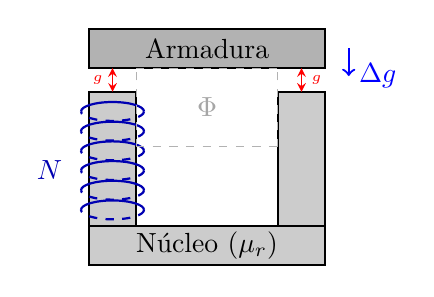
\begin{tikzpicture}[scale=1]
    % Núcleo en U (parte inferior)
    \draw[fill=gray!40, thick] (0,0) rectangle (3, 0.5);      % base
    \draw[fill=gray!40, thick] (0,0.5) rectangle (0.6, 2.2);  % pilar izq
    \draw[fill=gray!40, thick] (2.4,0.5) rectangle (3, 2.2);  % pilar der

    % Bobina en el pilar izquierdo
    \foreach \y in {0.7, 0.95, 1.2, 1.45, 1.7, 1.95} {
        \draw[blue!70!black, thick] (-0.1,\y) arc[start angle=180, end angle=0,
                                              x radius=0.4, y radius=0.12];
        \draw[blue!70!black, dashed, thick] (0.7,\y) arc[start angle=0, end angle=-180, x radius=0.4, y radius=0.12];
    }

    \node[blue!70!black] at (-0.5, 1.2) {$N$};

    % Armadura móvil (parte superior)
    \draw[fill=gray!60, thick] (0,2.5) rectangle (3, 3.0);

    % Entrehierro
    \draw[<->, red, >=stealth] (0.3, 2.2) -- (0.3, 2.5)
          node[midway, left, font=\tiny, red] {$g$};
    \draw[<->, red, >=stealth] (2.7, 2.2) -- (2.7, 2.5)
          node[midway, right, font=\tiny, red] {$g$};

    % Flecha de movimiento
    \draw[->, thick, blue] (3.3, 2.75) -- (3.3, 2.4)
          node[right] {$\Delta g$};

    % Etiquetas
    \node[] at (1.5, 0.25) {Núcleo ($\mu_r$)};
    \node[] at (1.5, 2.75) {Armadura};

    % Líneas de flujo (punteadas)
    \draw[dashed, gray!60] (0.6, 1.5) -- (0.6, 2.5);
    \draw[dashed, gray!60] (2.4, 1.5) -- (2.4, 2.5);
    \draw[dashed, gray!60] (0.6, 2.5) -- (2.4, 2.5);
    \draw[dashed, gray!60] (0.6, 1.5) -- (2.4, 1.5);
    \node[gray!70] at (1.5, 2.0) {$\Phi$};
  \end{tikzpicture}
  \caption[Sensor de reluctancia variable.]{Sensor de reluctancia variable. El desplazamiento de la armadura modifica el entrehierro $g$ y, por tanto, la inductancia $L$ de la bobina.}\label{fig:reluctancia}
\end{marginfigure}

\paragraph{Curva de Transferencia y No Linealidad}

La Figura~\ref{fig:curva_reluctancia} muestra la respuesta $L$ frente a $g$ para el modelo de la ecuación~\eqref{eq:L_vs_g}. Como en los sensores capacitivos de distancia, la alta sensibilidad en el origen (entrehierros pequeños) se paga con una respuesta no lineal. 

Para resolver este problema, se propone un modelo de \emph{configuración diferencial}. La \emph{configuración diferencial de reluctancia variable} con dos bobinas ($L_1, L_2$) en estructura push-pull linealiza la respuesta y duplica la sensibilidad, siguiendo la misma álgebra que el condensador diferencial. Sin embargo, esta solución es más compleja de implementar que en el caso capacitivo, ya que requiere un diseño mecánico preciso para garantizar la simetría de las bobinas y el movimiento de la armadura.

\begin{marginfigure}
  \centering
  \shorthandoff{>}
  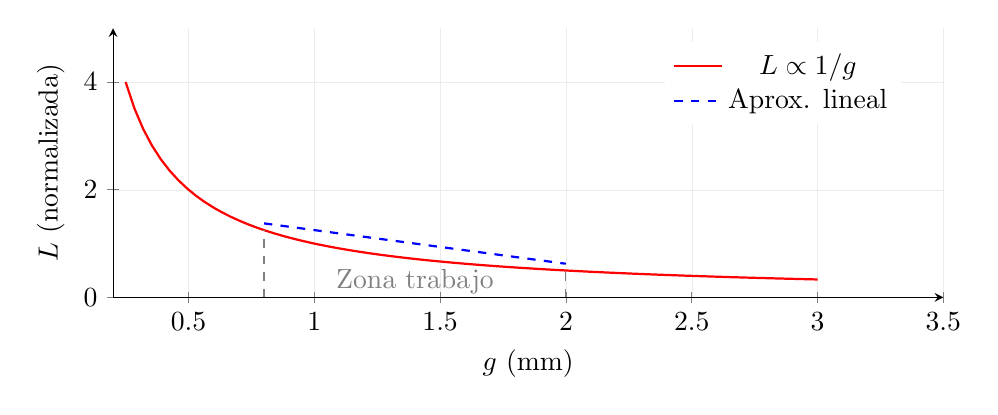
\begin{tikzpicture}
    \begin{axis}[
      width=\linewidth, height=5cm,
      xlabel={$g$ (\unit{mm})},
      ylabel={$L$ (normalizada)},
      xmin=0.2, xmax=3.5,
      ymin=0, ymax=5,
      axis lines=left, grid=both,
      grid style={line width=.1pt, draw=gray!15},
      legend style={at={(0.95,0.95)}, anchor=north east, draw=none}
    ]
      % L ∝ 1/g
      \addplot[thick, red, domain=0.25:3, samples=80] {1/x};
      \addlegendentry{$L \propto 1/g$}

      % Zona lineal aproximada
      \addplot[thick, blue, dashed, domain=0.8:2.0, samples=2]
              {-0.625*x + 1.875};
      \addlegendentry{Aprox. lineal}

      \draw[gray, dashed] (axis cs:0.8,0) -- (axis cs:0.8, 1.25);
      \draw[gray, dashed] (axis cs:2.0,0) -- (axis cs:2.0, 0.625);
      \node[ gray] at (axis cs:1.4, 0.3) {Zona trabajo};
    \end{axis}
  \end{tikzpicture}
  \caption[Respuesta $L(g)$ del sensor de reluctancia variable.]{Respuesta $L(g)$ del sensor de reluctancia variable. Solo en un entorno reducido del punto de operación la curva puede aproximarse por una recta.}\label{fig:curva_reluctancia}
\end{marginfigure}

Los sensores de efecto Hall activos han reemplazado progresivamente a los de reluctancia variable en los \emph{Anti-lock Braking System} (ABS) modernos, ya que funcionan desde velocidad cero (el sensor pasivo de reluctancia variable requiere una velocidad mínima de \qty{2}{km/h} para generar señal), y su salida digital (tren de pulsos de amplitud constante) es inmune al ruido electromagnético del entorno del vehículo.

\paragraph{Aplicaciones}

Los sensores de reluctancia variable son la base de los \emph{encoders de efecto magnético} para medida de posición angular en motores de corriente continua y los \emph{sensores de velocidad de rueda}  ABS en automoción, donde la frecuencia de los pulsos generados es proporcional a la velocidad de rotación.  Como se muestra en la Figura \ref{fig:abs_sensor}, una rueda dentada ferromagnética gira junto a la rueda del coche, y el sensor de reluctancia variable genera un pulso eléctrico cada vez que un diente pasa por delante. La frecuencia de esos pulsos es proporcional a la velocidad de rotación de la rueda. La \emph{Electronic Control Unit} (ECU) del ABS monitoriza las cuatro ruedas continuamente y, si detecta que una se frena bruscamente (frecuencia cae a cero → rueda bloqueada), modula la presión hidráulica del freno para evitar el deslizamiento.

% \begin{marginfigure}[0em]
%   \centering
%   \shorthandoff{>}
%   \begin{tikzpicture}[scale=1.0]

%     % --- Disco dentado (reluctor) ---
%     % Radio interior y exterior del disco
%     \def\Ri{1.0}   % radio interior (alma del disco)
%     \def\Ro{1.45}  % radio exterior (punta del diente)
%     \def\Nd{12}    % número de dientes visibles (simplificado)

%     % Alma del disco
%     \fill[gray!40] (0,0) circle (\Ri);
%     \draw[thick]   (0,0) circle (\Ri);

%     % Dientes: cada diente ocupa 360/Nd grados, la mitad es diente
%     % y la mitad es hueco. Se dibujan como sectores anulares.
%     \foreach \i in {0,1,...,11} {
%       \pgfmathsetmacro{\angA}{\i * 360/\Nd}
%       \pgfmathsetmacro{\angB}{\angA + 0.5*360/\Nd}
%       % Diente (sólido)
%       \fill[gray!60]
%         (\angA:\Ri) arc[start angle=\angA, end angle=\angB,
%                         radius=\Ri]
%         -- (\angB:\Ro) arc[start angle=\angB, end angle=\angA,
%                            radius=\Ro]
%         -- cycle;
%       \draw[thick, gray!70]
%         (\angA:\Ri) arc[start angle=\angA, end angle=\angB,
%                         radius=\Ri]
%         -- (\angB:\Ro) arc[start angle=\angB, end angle=\angA,
%                            radius=\Ro]
%         -- cycle;
%     }

%     % Eje central
%     \fill[gray!80] (0,0) circle (0.18);
%     \draw[thick]   (0,0) circle (0.18);

%     % Flecha de rotación
%     \draw[->, thick, red!70!black, >=stealth]
%       (0, 1.75) arc[start angle=90, end angle=20, radius=1.75]
%       node[midway, above right, font=\tiny, red!70!black] {$\omega$};

%     % --- Sensor de reluctancia variable ---
%     % Posicionado en la parte superior derecha (diente en posición ~75°)
%     \begin{scope}[shift={(1.85, 1.85)}, rotate=-45]

%       % Cuerpo del sensor (carcasa)
%       \fill[blue!15]  (-0.22, 0) rectangle (0.22, 0.65);
%       \draw[thick]    (-0.22, 0) rectangle (0.22, 0.65);

%       % Polo magnético (núcleo)
%       \fill[gray!60]  (-0.12, 0) rectangle (0.12, 0.30);

%       % Bobina (espiras simplificadas)
%       \foreach \yy in {0.08, 0.15, 0.22} {
%         \draw[blue!70!black, thick]
%           (-0.22, \yy) arc[start angle=180, end angle=0,
%                            x radius=0.22, y radius=0.055];
%         \draw[blue!70!black, dashed, thick, opacity=0.5]
%           (-0.22, \yy) arc[start angle=180, end angle=360,
%                            x radius=0.22, y radius=0.055];
%       }

%       % Conector (cable)
%       \draw[thick, gray!60] (0, 0.65) -- (0, 1.0);
%       \fill[gray!50] (-0.08, 1.0) rectangle (0.08, 1.12);

%     \end{scope}

%     % Entrehierro entre sensor y diente (flecha roja)
%     \draw[<->, red, >=stealth, thick]
%       (0.98, 1.40) -- (1.25, 1.60)
%       node[midway, above left, font=\tiny, red] {$g$};

%     % Etiquetas
%     \node[font=\tiny, align=center] at (0, -1.75)
%       {Reluctor ($n=48$ dientes)};
%     \node[font=\tiny, blue!70!black, align=center] at (2.5, 2.6)
%       {Sensor};

%   \end{tikzpicture}
%   \caption[Sensor de velocidad de rueda ABS.]{Sensor de velocidad de rueda ABS. El reluctor gira
%     solidario a la rueda; el sensor de reluctancia variable genera
%     un pulso por cada diente. La UCE del ABS calcula $v$ a partir
%     de la frecuencia de pulsos mediante la
%     ec.~\eqref{eq:abs_freq}.}\label{fig:abs_sensor}
% \end{marginfigure}

\begin{marginfigure}[0em]
  \centering
  \shorthandoff{>}
  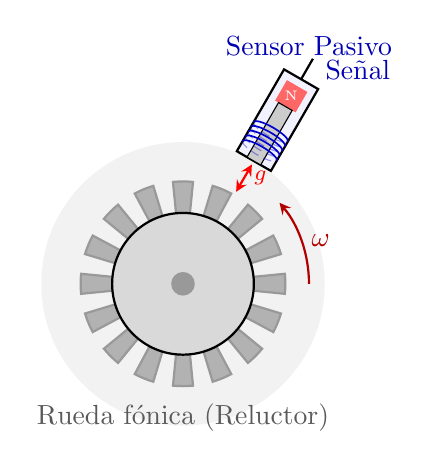
\begin{tikzpicture}[
    scale=1, 
    %font=\scriptsize,
    >=stealth,
    diente/.style={fill=gray!60, draw=gray!80, thick},
    alma/.style={fill=gray!30, draw=black, thick}
  ]

    % --- Parámetros Geométricos ---
    \def\Ri{0.9}    % Radio interior
    \def\Ro{1.3}    % Radio exterior (dientes)
    \def\Nd{16}     % Número de dientes para que se vea más denso
    \def\angSensor{60} % Ángulo donde situamos el sensor

    % --- Disco dentado (Reluctor) ---
    \fill[gray!10] (0,0) circle (\Ro + 0.5); % Fondo sutil para dar contexto
    
    % Dibujo de los dientes
    \foreach \i in {0,1,...,\numexpr\Nd-1\relax} {
      \pgfmathsetmacro{\angInicio}{\i * 360/\Nd - (360/\Nd)/4}
      \pgfmathsetmacro{\angFin}{\i * 360/\Nd + (360/\Nd)/4}
      
      \fill[gray!60] (\angInicio:\Ri) -- (\angInicio:\Ro) 
        arc (\angInicio:\angFin:\Ro) -- (\angFin:\Ri) 
        arc (\angFin:\angInicio:\Ri) -- cycle;
      \draw[gray!80, thick] (\angInicio:\Ri) -- (\angInicio:\Ro) 
        arc (\angInicio:\angFin:\Ro) -- (\angFin:\Ri) 
        arc (\angFin:\angInicio:\Ri);
    }
    
    % Alma del disco (círculo interior)
    \draw[alma] (0,0) circle (\Ri);
    \fill[gray!80] (0,0) circle (0.15); % Eje

    % Flecha de rotación omega
    \draw[->, thick, red!70!black] (0:1.6) arc (0:40:1.6) 
      node[midway, right, red!70!black] {$\omega$};

    % --- Sensor de Reluctancia Variable ---
    % Situado exactamente sobre el diente en \angSensor
    \begin{scope}[shift={(\angSensor:1.8)}, rotate=\angSensor-90]
      
      % Carcasa del sensor
      \draw[fill=blue!5, thick] (-0.25, 0) rectangle (0.25, 1.2);
      
      % Imán permanente (parte trasera)
      \fill[red!60] (-0.15, 0.8) rectangle (0.15, 1.1);
      \node[white, font=\tiny] at (0, 0.95) {N};
      
      % Núcleo de hierro (Polo)
      \fill[gray!40, draw=black] (-0.1, 0) rectangle (0.1, 0.8);
      
      % Bobina (Windings) - Representación más densa
      \foreach \y in {0.15, 0.22, 0.29, 0.36, 0.43} {
        \draw[blue!80!black, semithick] (-0.25, \y) arc (180:0:0.25 and 0.06);
        \draw[blue!80!black, densely dashed, opacity=0.4] (-0.25, \y) arc (180:360:0.25 and 0.06);
      }
      
      % Salida de cables
      \draw[thick] (0, 1.2) -- (0, 1.5) coordinate (finalCable);
      \node[blue!70!black, right] at (0.1, 1.4) {Señal};
    \end{scope}

    % --- Detalles de medida ---
    % Entrehierro g (medido desde la punta del diente al núcleo)
    \draw[<->, red, thick] (\angSensor:\Ro + 0.05) -- (\angSensor:1.8 - 0.05)
      node[midway, right, font=\footnotesize\bfseries] {$g$};

    % Etiquetas de componentes
    \node[anchor=north, gray!70!black] at (0,-1.4) {Rueda fónica (Reluctor)};
    \node[anchor=south, blue!70!black] at (\angSensor:3.2) {Sensor Pasivo};

  \end{tikzpicture}
  \caption[Sensor de velocidad de rueda ABS.]{Sensor de velocidad de rueda ABS (Rueda fónica). El movimiento de los dientes altera la reluctancia del circuito magnético del sensor, induciendo una tensión alterna cuya frecuencia es proporcional a la velocidad angular de la rueda.}\label{fig:abs_sensor}
\end{marginfigure}

% ------- Marginnote: funcionamiento del ABS -------
\marginnote{\textbf{Cómo actúa el ABS:} La Unidad de Control Electrónico (UCE) monitoriza las cuatro ruedas simultáneamente. Si durante una frenada la frecuencia de una rueda cae a cero mientras las demás siguen girando, la UCE detecta \emph{bloqueo inminente} y activa el módulo hidráulico: reduce la presión de frenado en esa rueda ($\approx \qty{20}{ms}$), la deja recuperar velocidad y vuelve a aplicar presión. Este ciclo (\emph{reduce\,--\,mantiene\,--\,aumenta}) se repite a \qtyrange{8}{15}{\hertz}, manteniendo la rueda en el rango de deslizamiento óptimo ($\lambda \approx \qty{15}{\percent}$) donde la adherencia neumático-asfalto es máxima.%
}

% -----------------------------------------------------------
\subsection{Transformador Diferencial de Variación Lineal (LVDT)}\label{sub:lvdt}
% -----------------------------------------------------------

El \emph{Linear Variable Differential Transformer} (LVDT) es el sensor de desplazamiento de referencia en instrumentación de precisión. Combina la ausencia de contacto mecánico, la robustez intrínseca de los sensores inductivos y una respuesta \emph{intrínsecamente lineal} en un amplio rango. Se emplea en ensayos de materiales, control de turbinas de aviación y microscopía de fuerza atómica.

\paragraph{Estructura Interna}

\begin{marginfigure}[0em]
  \centering
  \shorthandoff{>}
  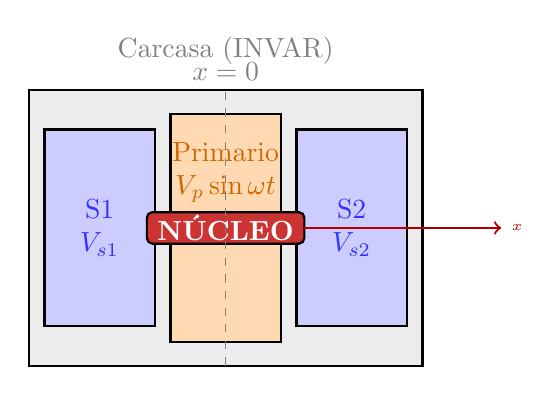
\begin{tikzpicture}[scale=1]
    % Cuerpo del LVDT (sección transversal)
    \draw[fill=gray!15, thick] (0,0) rectangle (5, 3.5);
    \node[gray] at (2.5, 4) {Carcasa (INVAR)};

    % Bobina primaria (centro)
    \draw[fill=orange!30, thick] (1.8, 0.3) rectangle (3.2, 3.2);
    \node[orange!80!black, align=center, above] at (2.5, 1.95)
         {Primario\\$V_p \sin\omega t$};

    % Bobina secundaria 1 (izquierda)
    \draw[fill=blue!20, thick] (0.2, 0.5) rectangle (1.6, 3.0);
    \node[blue!80, align=center] at (0.9, 1.75) {S1\\$V_{s1}$};

    % Bobina secundaria 2 (derecha)
    \draw[fill=blue!20, thick] (3.4, 0.5) rectangle (4.8, 3.0);
    \node[blue!80,align=center] at (4.1, 1.75) {S2\\$V_{s2}$};

    % Núcleo ferromagnético
    \draw[fill=red!60!gray, thick, rounded corners=2pt]
         (1.5, 1.55) rectangle (3.5, 1.95);
    \node[white, font=\bfseries] at (2.5, 1.75) {NÚCLEO};

    % Varilla de accionamiento
    \draw[thick, red!70!black] (3.5, 1.75) -- (5.5, 1.75);
    \draw[->, thick, red!70!black] (5.5, 1.75) -- (6.0, 1.75)
          node[right, font=\tiny] {$x$};

    % Posición nula
    \draw[dashed, gray] (2.5, 0) -- (2.5, 3.5)
          node[above, gray] {$x=0$};
  \end{tikzpicture}
  \caption{Sección transversal del LVDT. El primario está alimentado con una señal alterna. Las dos secundarias están conectadas en oposición de serie. La varilla de accionamiento controla la posición del núcleo ferromagnético. El núcleo ferromagnético se encuentra en la sección transversal.}\label{fig:lvdt_estructura}
\end{marginfigure}

Como se muestra en la figura~\ref{fig:lvdt_estructura}, el LVDT consta de tres bobinas coaxiales: un \emph{primario} central excitado con $V_p \sin(\omega t)$ (tipicamente entre \qty{1}{kHz} y \qty{10}{kHz}) y dos \emph{secundarios} (S1 y S2) situados simétricamente a ambos lados, conectados en oposición de serie:

\begin{equation}\label{eq:v_out_lvdt}
    V_{out} = V_{S1} - V_{S2}
\end{equation}

\paragraph{Análisis de Transferencia}

El acoplamiento mutuo entre el primario y cada secundario depende de la posición del núcleo ferromagnético:

\begin{equation}
    M_1(x) = M_0 + k \cdot x \qquad ; \qquad M_2(x) = M_0 - k \cdot x
\end{equation}

donde $k$ es una constante de sensibilidad geométrica y $x$ el desplazamiento del núcleo. Las tensiones inducidas son $V_{S1} \propto M_1$ y $V_{S2} \propto M_2$, por lo que la salida diferencial resulta:

\begin{equation}\label{eq:lvdt_lineal}
    V_{out}(x) = 2k \cdot x \cdot V_p \sin(\omega t + \phi)
\end{equation}

La ecuación~\eqref{eq:lvdt_lineal} revela dos propiedades fundamentales del LVDT:

\begin{enumerate}
    \item \emph{Linealidad perfecta:} La amplitud de $V_{out}$ es estrictamente proporcional a $x$.
    \item \emph{Información de dirección en la fase:} Para $x > 0$, $V_{out}$ está en fase con $V_p$ ($\phi = 0°$); para $x < 0$, $V_{out}$ se invierte ($\phi = 180°$). Un simple voltímetro de valor eficaz \emph{no puede distinguir} la dirección; se requiere \emph{demodulación síncrona}.
\end{enumerate}

\marginnote{\textbf{Punto nulo eléctrico:} En la posición central ($x=0$), la salida ideal es $V_{out} = 0$. En la práctica, siempre existe una pequeña tensión residual de cuadratura (en fase con $dV_p/dt$) debida a acoplamientos capacitivos parásitos entre bobinas. Esta tensión de cuadratura es el indicador de calidad de fabricación del LVDT.}

\begin{marginfigure}
  \centering
  \shorthandoff{>}
  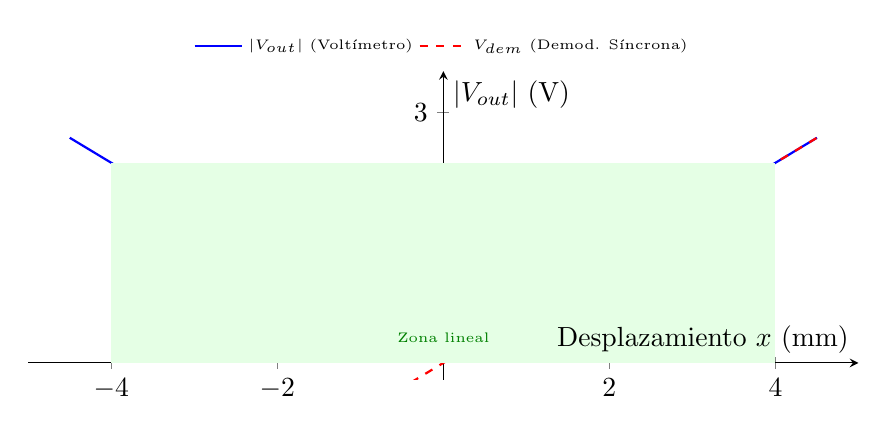
\begin{tikzpicture}
    \begin{axis}[
      width=\linewidth, height=5.5cm,
      xlabel={Desplazamiento $x$ (mm)},
      ylabel={$|V_{out}|$ (V)},
      xmin=-5, xmax=5,
      ymin=-0.2, ymax=3.5,
      axis lines=center,
      xtick={-4,-2,0,2,4},
      ytick={0,1,2,3},
      legend style={at={(0.5,1.02)}, anchor=south,
                    legend columns=2, draw=none, font=\tiny}
    ]
      % Salida ideal (módulo = V-forma)
      \addplot[thick, blue, domain=-4.5:4.5, samples=100]
              {abs(0.6*x)};
      \addlegendentry{$|V_{out}|$ (Voltímetro)}

      % Salida con signo (demodulada)
      \addplot[thick, red, dashed, domain=-4.5:4.5, samples=100]
              {0.6*x};
      \addlegendentry{$V_{dem}$ (Demod. Síncrona)}

      % Zona lineal
      \fill[green!10] (axis cs:-4,0) rectangle (axis cs:4,2.4);
      \node[green!50!black, font=\tiny] at (axis cs:0, 0.3)
           {Zona lineal};
    \end{axis}
  \end{tikzpicture}
  \caption{Curvas de transferencia del LVDT. Sin demodulación síncrona solo se obtiene el módulo (azul). La detección de fase proporciona el desplazamiento con signo (rojo).}\label{fig:lvdt_curvas}
\end{marginfigure}

La Tabla~\ref{tab:lvdt_pros_cons} resume las ventajas e inconvenientes del LVDT para el diseñador de sistemas de instrumentación. Su linealidad intrínseca y robustez lo convierten en la opción preferida para aplicaciones de alta precisión, aunque su complejidad de señal y sensibilidad a campos magnéticos externos pueden ser limitantes en entornos industriales ruidosos.

\begin{table}[ht]
  \centering
  \small
  \begin{tabularx}{\linewidth}{X X}
    \toprule
    \textbf{Ventajas} & \textbf{Inconvenientes} \\
    \midrule
    Sin contacto mecánico: vida infinita & Requiere electrónica de demodulación síncrona \\
    Linealidad $< 0.1\%$ del fondo de escala & Sensible a campos magnéticos externos \\
    Resolución ilimitada (solo limitada por ruido) & Frecuencia de excitación fija por diseño \\
    Robusto a vibración, temperatura y polvo & Mayor tamaño que sensores capacitivos MEMS \\
    \bottomrule
  \end{tabularx}
  \caption{Comparativa de ventajas e inconvenientes del LVDT para el diseñador de sistemas de instrumentación.}\label{tab:lvdt_pros_cons}
\end{table}

\paragraph{Rangos típicos de especificación}

Un LVDT industrial estándar (p.ej. familia HCD de Sensata o Series 100 de Measurement Specialties) presenta: rango de $\pm$\qty{0.5}{mm} a $\pm$\qty{500}{mm}, linealidad mejor del \qty{0.25}{\%} F.E., resolución en el orden de \qty{1}{\micro m} con electrónica de 16~bits, y temperatura de operación de \qtyrange{-55}{150}{\degreeCelsius}.

% -----------------------------------------------------------
\subsection{Sensores de Corrientes de Foucault (\textit{Eddy Currents})}\label{sub:eddy}
% -----------------------------------------------------------

\paragraph{Fenómeno Físico}

Cuando un conductor eléctrico (no necesariamente ferromagnético) se introduce en un campo magnético variable, la Ley de Faraday induce en su interior corrientes circulares denominadas \emph{corrientes de Foucault} o \emph{eddy currents}. Estas corrientes generan, a su vez, un campo magnético opuesto al inductor (Lenz), modificando la impedancia efectiva de la bobina de excitación:

\begin{equation}\label{eq:z_eddy}
  Z_{ef\!f}(\delta) = R_0 + j\omega L_0 + \Delta Z(\delta)
\end{equation}

donde $\delta$ es la distancia entre la bobina y el conductor objetivo (\textit{target}), y $\Delta Z(\delta)$ es la perturbación de impedancia debida a las corrientes de Foucault. En la práctica, $\Delta Z$ reduce tanto la parte real (pérdidas en el target) como la parte imaginaria (pérdidas de inductancia).

\begin{marginfigure}[0em]
  \centering
  \shorthandoff{>}
  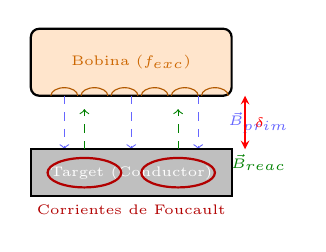
\begin{tikzpicture}[scale=0.85]
    % Bobina de excitación
    \draw[fill=orange!20, thick, rounded corners=3pt]
         (0, 2.0) rectangle (3, 3.0);
    \foreach \x in {0.3, 0.75, 1.2, 1.65, 2.1, 2.55} {
      \draw[orange!70!black] (\x, 2.0) arc[start angle=180, end angle=0,
                                           x radius=0.2, y radius=0.12];
    }
    \node[font=\tiny, orange!80!black] at (1.5, 2.5) {Bobina ($f_{exc}$)};

    % Flujo primario (flechas azules hacia abajo)
    \foreach \x in {0.5, 1.5, 2.5} {
      \draw[->, blue!60, dashed] (\x, 2.0) -- (\x, 1.2);
    }
    \node[blue!60, font=\tiny] at (3.4, 1.6) {$\vec{B}_{prim}$};

    % Entrehierro
    \draw[<->, red, >=stealth] (3.2, 1.2) -- (3.2, 2.0)
          node[midway, right, font=\tiny, red] {$\delta$};

    % Target conductor
    \draw[fill=gray!50, thick] (0, 0.5) rectangle (3, 1.2);
    \node[font=\tiny, white] at (1.5, 0.85) {Target (Conductor)};

    % Corrientes de Foucault (elipses rojas)
    \draw[thick, red!70!black, ->]
         (0.8, 0.85) ellipse (0.55cm and 0.22cm);
    \draw[thick, red!70!black, ->]
         (2.2, 0.85) ellipse (0.55cm and 0.22cm);
    \node[red!70!black, font=\tiny] at (1.5, 0.3) {Corrientes de Foucault};

    % Campo de reacción (flechas hacia arriba)
    \foreach \x in {0.8, 2.2} {
      \draw[->, green!50!black, dashed] (\x, 1.2) -- (\x, 1.8);
    }
    \node[green!50!black, font=\tiny] at (3.4, 1.0) {$\vec{B}_{reac}$};
  \end{tikzpicture}
  \caption{Principio de los sensores de corrientes de Foucault. Las corrientes inducidas en el target crean un campo de reacción que modifica la impedancia de la bobina como función de $\delta$.}\label{fig:eddy_principio}
\end{marginfigure}

\paragraph{Profundidad de Penetración (\textit{Skin Depth})}

Las corrientes de Foucault no se distribuyen uniformemente en el conductor: se concentran en la superficie. La \emph{profundidad de penetración} $\delta_{skin}$ define la capa efectiva donde circula el \qty{63}{\%} de la corriente total:

\begin{equation}\label{eq:skin_depth}
  \delta_{skin} = \sqrt{\frac{2\rho}{\omega \mu_0 \mu_r}} = \sqrt{\frac{\rho}{\pi f \mu_0 \mu_r}}
\end{equation}

donde $\rho$ es la resistividad del material y $f$ la frecuencia de excitación.

\marginnote{\textbf{Implicación de diseño:} La frecuencia de excitación determina la profundidad de análisis. A \qty{10}{kHz} en aluminio ($\rho = \qty{28}{n\Omega\cdot m}$), $\delta_{skin} \approx \qty{0.8}{mm}$. A \qty{1}{MHz}, $\delta_{skin} \approx \qty{0.08}{mm}$. Esto permite usar los sensores de Eddy Currents para \emph{END} (Ensayos No Destructivos): a baja frecuencia se detectan defectos internos; a alta frecuencia, solo superficiales.}

\begin{marginfigure}
  \centering
  \shorthandoff{>}
  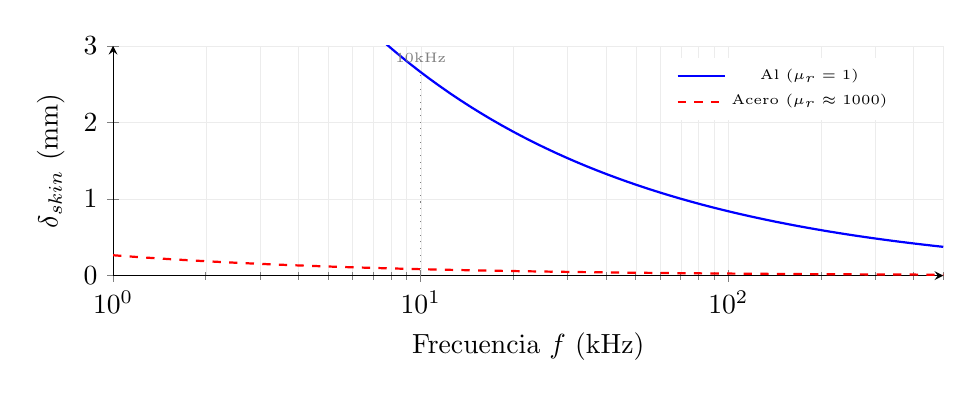
\begin{tikzpicture}
    \begin{axis}[
      width=\linewidth, height=4.5cm,
      xlabel={Frecuencia $f$ (kHz)},
      ylabel={$\delta_{skin}$ (\unit{mm})},
      xmin=1, xmax=500,
      ymin=0, ymax=3,
      xmode=log,
      axis lines=left, grid=both,
      grid style={line width=.1pt, draw=gray!15},
      legend style={at={(0.95,0.95)}, anchor=north east,
                    draw=none, font=\tiny}
    ]
      % Aluminio: delta = sqrt(rho/(pi*f*mu0)) con rho=2.8e-8, mu0=4pi*1e-7
      % delta_mm = sqrt(2.8e-8 / (pi * f*1e3 * 4*pi*1e-7)) * 1000
      % = sqrt(2.8e-8 / (1.2566e-6 * f*1e3)) * 1000
      % = sqrt(22.28e-3 / f) * 1000 = sqrt(22.28/f) * ... simplificamos:
      % delta = 8.4 / sqrt(f_kHz)  mm  (approx. para Al)
      \addplot[thick, blue, domain=1:500, samples=80] {8.4/sqrt(x)};
      \addlegendentry{Al ($\mu_r=1$)}

      % Acero: mu_r ≈ 1000, delta = 8.4/sqrt(1000*f) = 0.266/sqrt(f)
      \addplot[thick, red, dashed, domain=1:500, samples=80] {0.266/sqrt(x)};
      \addlegendentry{Acero ($\mu_r \approx 1000$)}

      % Linea guia
      \draw[gray, dotted] (axis cs:10, 0) -- (axis cs:10, 2.66)
           node[above, font=\tiny] {\qty{10}{kHz}};
    \end{axis}
  \end{tikzpicture}
  \caption{Profundidad de penetración $\delta_{skin}$ frente a frecuencia de excitación para aluminio y acero. El acero, al ser ferromagnético ($\mu_r \gg 1$), confina las corrientes en una capa mucho más delgada.}\label{fig:skin_depth}
\end{marginfigure}

\paragraph{Circuito Equivalente y Medida}

El sistema bobina + target puede modelarse como un transformador con el secundario cortocircuitado. La impedancia vista desde el primario tiene la forma:

\begin{equation}
  Z_{in} = \left(R_0 + \frac{\omega^2 M^2 R_t}{R_t^2 + \omega^2 L_t^2}\right)
           + j\omega\left(L_0 - \frac{\omega^2 M^2 L_t}{R_t^2 + \omega^2 L_t^2}\right)
\end{equation}

Ambas partes (resistiva e inductiva) dependen de $\delta$ a través del acoplamiento mutuo $M(\delta) \propto e^{-\delta/\delta_0}$. En la práctica, la medida se realiza mediante un \emph{analizador de impedancias} o un \emph{circuito resonante} donde se monitoriza el desplazamiento de la frecuencia de resonancia.

\paragraph{Características y Aplicaciones}

\begin{table}[ht]
  \centering
  \small
  \begin{tabularx}{\linewidth}{l X}
    \toprule
    \textbf{Parámetro} & \textbf{Valor típico} \\
    \midrule
    Rango de medida & \qtyrange{0.5}{30}{mm} \\
    Resolución & $<\qty{1}{\micro m}$ \\
    Frecuencia de excitación & \qtyrange{1}{10}{MHz} \\
    Materiales target & Cualquier conductor (Al, Cu, acero, Ti) \\
    Temperatura de operación & \qtyrange{-50}{200}{\degreeCelsius} \\
    Inmunidad a contaminantes & Aceite, polvo, agua: \textbf{total} \\
    \bottomrule
  \end{tabularx}
  \caption{Especificaciones típicas de los sensores de corrientes de Foucault industriales (familia Micro-Epsilon eddyNCDT).}\label{tab:eddy_specs}
\end{table}

Sus principales aplicaciones en ingeniería de telecomunicaciones e industrial son: medida de espesor de recubrimientos no conductores sobre metal, detección de grietas subsuperficiales en piezas aeronáuticas (\emph{END}), medida de desplazamiento de ejes en rodamientos magnéticos y control de calidad de placas PCB (grosor del cobre).

% -----------------------------------------------------------
\subsection{Sensores de Efecto Hall y Magnetorresistivos}\label{sub:hall_mr}
% -----------------------------------------------------------

\paragraph{Efecto Hall}

Cuando una corriente $I$ fluye por un conductor situado en un campo magnético $\vec{B}$ perpendicular, la fuerza de Lorentz ($\vec{F} = q\vec{v} \times \vec{B}$) desvía los portadores de carga acumulándose en las caras laterales del conductor hasta establecer un campo eléctrico transversal que equilibra la fuerza magnética. La tensión de Hall resultante es:

\begin{equation}\label{eq:v_hall}
  V_H = \frac{R_H \cdot I \cdot B}{t} = \frac{I \cdot B}{n_e \cdot q \cdot t}
\end{equation}
%
donde $R_H = 1/(n_e q)$ es la constante de Hall del material ($n_e$ densidad de portadores, $q$ carga del electrón) y $t$ el espesor del conductor.

% \begin{marginfigure}[1em]
%   \centering
%   \shorthandoff{>}
%   \begin{tikzpicture}[scale=0.8]
%     % Plaqueta de Hall (paralelepípedo)
%     \draw[fill=blue!15, thick]
%       (0.5, 0.5) -- (2.5, 0.5) -- (3.0, 1.0) --
%       (1.0, 1.0) -- cycle;                          % cara superior
%     \draw[fill=blue!25, thick]
%       (0.5, 0.5) -- (0.5, 2.5) -- (1.0, 3.0) --
%       (1.0, 1.0) -- cycle;                          % cara izquierda
%     \draw[fill=blue!10, thick]
%       (0.5, 2.5) -- (2.5, 2.5) -- (3.0, 3.0) --
%       (1.0, 3.0) -- cycle;                          % cara frontal
%     \draw[fill=blue!20, thick]
%       (2.5, 0.5) -- (2.5, 2.5) -- (3.0, 3.0) --
%       (3.0, 1.0) -- cycle;                          % cara derecha
%     \draw[fill=blue!5, thick]
%       (0.5, 0.5) -- (2.5, 0.5) -- (2.5, 2.5) --
%       (0.5, 2.5) -- cycle;                          % cara frontal

%     % Corriente I (horizontal, rojo)
%     \draw[->, thick, red] (-0.3, 1.5) -- (0.5, 1.5)
%           node[above, font=\tiny, red] {$I$};
%     \draw[->, thick, red] (2.5, 1.5) -- (3.3, 1.5);

%     % Campo B (vertical, verde, hacia arriba)
%     \draw[->, thick, green!60!black] (1.5, -0.2) -- (1.5, 0.5)
%           node[below left, font=\tiny, green!60!black] {$\vec{B}$};
%     \draw[->, thick, green!60!black] (1.5, 2.5) -- (1.5, 3.2);

%     % Tensión Hall (azul, lateral)
%     \draw[<->, thick, blue] (0.1, 0.8) -- (0.1, 2.2)
%           node[midway, left, font=\tiny, blue] {$V_H$};

%     % Espesor t
%     \draw[<->, gray] (2.7, 0.5) -- (2.7, 2.5)
%           node[midway, right, font=\tiny, gray] {$t$};
%   \end{tikzpicture}
%   \caption{Geometría del efecto Hall. La corriente $I$ fluye horizontalmente; el campo $\vec{B}$ es perpendicular. Los portadores se acumulan generando $V_H$ en la dirección transversal.}\label{fig:hall_geometria}
% \end{marginfigure}

% \begin{marginfigure}[2em]
%   \centering
%   \shorthandoff{>}
%   \begin{tikzpicture}[
%     x=(10:2cm), y=(90:1.5cm), z=(210:1.0cm), % Perspectiva isométrica
%     font=\scriptsize,
%     >=stealth
%   ]

%     % --- Parámetros de la plaqueta ---
%     \def\w{2.0} % ancho
%     \def\h{0.6} % alto
%     \def\t{1.2} % espesor (profundidad)

%     % --- Dibujo de la plaqueta (Slab) ---
%     % Cara inferior
%     \fill[blue!5] (0,0,0) -- (\w,0,0) -- (\w,0,\t) -- (0,0,\t) -- cycle;
    
%     % Cara trasera
%     \fill[blue!10] (0,0,\t) -- (\w,0,\t) -- (\w,\h,\t) -- (0,\h,\t) -- cycle;
    
%     % Cara izquierda
%     \fill[blue!15] (0,0,0) -- (0,0,\t) -- (0,\h,\t) -- (0,\h,0) -- cycle;

%     % Cara frontal
%     \fill[blue!20, opacity=0.8] (0,0,0) -- (\w,0,0) -- (\w,\h,0) -- (0,\h,0) -- cycle;
%     \draw[thick, blue!80!black] (0,0,0) -- (\w,0,0) -- (\w,\h,0) -- (0,\h,0) -- cycle;

%     % Cara superior
%     \fill[blue!10, opacity=0.8] (0,\h,0) -- (\w,\h,0) -- (\w,\h,\t) -- (0,\h,\t) -- cycle;
%     \draw[thick, blue!80!black] (0,\h,0) -- (\w,\h,0) -- (\w,\h,\t) -- (0,\h,\t) -- cycle;
%     \draw[thick, blue!80!black] (\w,0,0) -- (\w,0,\t) -- (\w,\h,\t) -- (\w,\h,0);
%     \draw[thick, blue!80!black] (0,\h,\t) -- (\w,\h,\t);

%     % --- Vectores ---

%     % Corriente I (Eje X)
%     \draw[ultra thick, red, ->] (-0.5, \h/2, \t/2) -- (0, \h/2, \t/2) node[pos=0, left] {$I$};
%     \draw[red, dashed] (0, \h/2, \t/2) -- (\w, \h/2, \t/2);
%     \draw[ultra thick, red, ->] (\w, \h/2, \t/2) -- (\w+0.5, \h/2, \t/2);

%     % Campo Magnético B (Eje Z - Entrante)
%     \foreach \x in {0.5, 1.5} {
%         \draw[ultra thick, green!60!black, ->] (\x, \h+0.5, \t+0.5) -- (\x, \h+0.5, \t-0.5) 
%               node[pos=0, above] {$\vec{B}$};
%     }

%     % Portadores y Fuerza de Lorentz (Cargas negativas acumuladas al frente)
%     \foreach \z in {0.2, 0.6, 1.0} {
%         \node[blue!80!black, font=\tiny] at (0.3, \h-0.15, 0) {$-$};
%         \node[red!80!black, font=\tiny] at (0.3, 0.15, 0) {$+$};
%     }

%     % --- Tensión de Hall V_H (Eje Y) ---
%     \draw[<->, blue, thick] (-0.3, 0, 0) -- (-0.3, \h, 0) 
%           node[midway, left] {$V_H$};
    
%     % --- Dimensiones ---
%     \draw[<->, gray] (\w, -0.2, 0) -- (\w, -0.2, \t) node[midway, below right] {$d$};
%     \draw[<->, gray] (0, -0.2, 0) -- (\w, -0.2, 0) node[midway, below] {$w$};

%   \end{tikzpicture}
%   \caption[Principio del Efecto Hall.]{Geometría del efecto Hall en un semiconductor tipo $n$. La aplicación de un campo magnético perpendicular $\vec{B}$ a la dirección de la corriente $I$ desvía los portadores de carga hacia las caras laterales debido a la fuerza de Lorentz, originando un campo eléctrico transversal y una diferencia de potencial $V_H$.}\label{fig:hall_geometria}
% \end{marginfigure}

% \begin{marginfigure}
%   \centering
%   \shorthandoff{>}
%   \begin{tikzpicture}[
%     x={(0:1cm)}, y={(90:1cm)}, z={(210:0.5cm)}, % Perspectiva
%     font=\scriptsize, >=stealth,
%     cargap/.style={circle, fill=red!20, draw=red, inner sep=0.5pt, font=\tiny},
%     cargan/.style={circle, fill=blue!20, draw=blue, inner sep=0.5pt, font=\tiny}
%   ]

%     % --- IMÁN SUPERIOR ---
%     \begin{scope}[shift={(1.5, 4, 0)}]
%         % Polo Norte (Rojo)
%         \fill[red!80!black] (-0.5, 0.5) rectangle (0.5, 1.2);
%         \node[white, font=\bfseries] at (0, 0.85) {N};
%         % Cuerpo imán
%         \fill[gray!20] (-0.5, -0.2) rectangle (0.5, 0.5);
%         % Polo Sur (Azul)
%         \fill[blue!80!black] (-0.5, -0.9) rectangle (0.5, -0.2);
%         \node[white, font=\bfseries] at (0, -0.55) {S};
%         \draw[thick] (-0.5, -0.9) rectangle (0.5, 1.2);
%         \node[above] at (0, 1.2) {Imán};
%     \end{scope}

%     % --- LÍNEAS DE FUERZA (B) ---
%     \foreach \x in {-0.4, -0.2, 0.2, 0.4} {
%         \draw[blue!60, dashed, ->] (1.5+\x, 3.1) .. controls (1.5+\x, 2.5) .. (1.5+\x, 1.1);
%     }
%     \node[right, blue!60, font=\tiny, align=left] at (2, 2.8) {Líneas de\\fuerza};

%     % --- ELEMENTO HALL (Plaqueta tipo P) ---
%     % Base
%     \fill[brown!40!black] (0,0,2) -- (3,0,2) -- (3,0,0) -- (0,0,0) -- cycle;
%     % Cuerpo (Semiconductor)
%     \fill[cyan!20, opacity=0.8] (0,0,2) -- (3,0,2) -- (3,0.3,2) -- (0,0.3,2) -- cycle; % Frontal
%     \fill[cyan!10, opacity=0.8] (0,0.3,2) -- (3,0.3,2) -- (3,0.3,0) -- (0,0.3,0) -- cycle; % Superior
%     \draw[thick, brown!40!black] (0,0,2) -- (3,0,2) -- (3,0.3,2) -- (0,0.3,2) -- cycle;
%     \draw[thick, brown!40!black] (0,0.3,2) -- (3,0.3,2) -- (3,0.3,0) -- (0,0.3,0) -- cycle;
%     \draw[thick, brown!40!black] (3,0,2) -- (3,0,0) -- (3,0.3,0) -- (3,0.3,2);

%     % --- PORTADORES Y CORRIENTE ---
%     \draw[->, purple, ultra thick] (0.5, 0.15, 1) -- (2.5, 0.15, 1) node[midway, above, font=\tiny] {Flujo de corriente constante};
    
%     % Acumulación de cargas (Huecos al fondo, electrones al frente por Lorentz)
%     % En tipo P, el campo B hacia abajo y v a la derecha desvía huecos (+) hacia atrás
%     \foreach \i in {0.5, 1.2, 2, 2.7} {
%         \node[cargap] at (\i, 0.4, 0.2) {+};
%         \node[cargan] at (\i, 0.4, 1.8) {-};
%     }
%     \node[anchor=east, font=\tiny] at (0, 0, 2) {Elemento Hall tipo P};

%     % --- CIRCUITO DE ALIMENTACIÓN (DC) ---
%     \draw (0, 0.15, 1) -- (-0.8, 0.15, 1) -- (-0.8, -1.5, 1) -- (0.5, -1.5, 1);
%     \draw (3, 0.15, 1) -- (3.8, 0.15, 1) -- (3.8, -1.5, 1) -- (1.5, -1.5, 1);
%     \begin{scope}[shift={(1, -1.5, 1)}]
%         \draw[thick] (0, -0.3) -- (0, 0.3); \draw[thick] (0.2, -0.15) -- (0.2, 0.15); % Batería
%         \node[below=0.2cm] at (0.1, 0) {Fuente DC};
%         \node[above left] at (0, 0) {+}; \node[above right] at (0.2, 0) {-};
%         \draw[->, purple] (1.5, 0.2) -- (0.8, 0.2) node[midway, above] {$i$};
%     \end{scope}

%     % --- CIRCUITO VOLTÍMETRO (V_H) ---
%     \fill[black] (1.5, 0.3, 0) circle (2pt); % Contacto atrás
%     \fill[black] (1.5, 0.3, 2) circle (2pt); % Contacto adelante
%     \draw (1.5, 0.3, 0) -- (4.5, 0.3, 0) -- (4.5, 0.5, 1);
%     \draw (1.5, 0.3, 2) -- (4.5, 0.3, 2) -- (4.5, 1.5, 1);
%     \draw (4.5, 1, 1) circle (0.3) node {$V_H$};
%     \node[right] at (4.8, 1, 1) {Tensión de Hall};
%     \node[blue, left] at (4.5, 1.5, 1) {+};
%     \node[blue, left] at (4.5, 0.5, 1) {-};

%   \end{tikzpicture}
%   \caption{Sensor de efecto Hall con semiconductor tipo P. El campo magnético vertical $H$ desvía los huecos y electrones hacia los laterales de la plaqueta, creando la tensión transversal $V_H$.}\label{fig:hall_completo}
% \end{marginfigure}

\begin{marginfigure}
  \centering
  \shorthandoff{>}
  \begin{tikzpicture}[
    x={(0:1cm)}, y={(90:1cm)}, z={(210:0.5cm)},
    font=\scriptsize, >=stealth,
    cargap/.style={circle, fill=red!20, draw=red, inner sep=0.5pt, font=\tiny},
    cargan/.style={circle, fill=blue!20, draw=blue, inner sep=0.5pt, font=\tiny}
  ]

    % --- CAMPO MAGNÉTICO (Vectores verticales atravesando) ---
    % Dibujamos algunos vectores detrás de la plaqueta
    \foreach \ix in {0.5, 1.5, 2.5} {
        \foreach \iz in {0.5, 1.5} {
            \draw[green!60!black, thick, ->] (\ix, -0.5, \iz) -- (\ix, 2.5, \iz);
        }
    }
    \node[green!60!black, font=\bfseries] at (2.8, 2.2, 0.5) {$\vec{B}$};

    \draw[->, purple, ultra thick] (-0.5, 0.2, 1) -- (3.5, 0.2, 1) 
          node[pos=0, left, font=\tiny, align=right] {Corriente\\constante ($I$)};

    % --- ELEMENTO HALL (Plaqueta tipo P) ---
    % Base (Cara inferior)
    %\fill[cyan!10, opacity=0.7] (0,0,2) -- (3,0,2) -- (3,0,0) -- (0,0,0) -- cycle;
    % FRONTAL (Semiconductor translúcido para ver el campo)
    \fill[cyan!10, opacity=0.7] (0,0,2) -- (3,0,2) -- (3,0.4,2) -- (0,0.4,2) -- cycle; 
    % ARRIBA
    \fill[cyan!10, opacity=0.7] (0,0.4,2) -- (3,0.4,2) -- (3,0.4,0) -- (0,0.4,0) -- cycle; % Superior
    % trasera
    %\fill[cyan!10, opacity=0.7] (0,0,0) -- (3,0,0) -- (3,0.4,0) -- (0,0.4,0) -- cycle;
    % LADO
    \fill[cyan!10, opacity=0.7] (3,0,2) -- (3,0,0) -- (3,0.4,0) -- (3,0.4,2) -- cycle; % Derecha

    % Aristas de la plaqueta
    % FRONTAL
    \draw[thick, brown!60!black] (0,0,2) -- (3,0,2) -- (3,0.4,2) -- (0,0.4,2) -- cycle;
    % ARRIBA
    \draw[thick, brown!60!black] (0,0.4,2) -- (3,0.4,2) -- (3,0.4,0) -- (0,0.4,0) -- cycle;
    % lado
    \draw[thick, brown!60!black] (3,0,2) -- (3,0,0) -- (3,0.4,0) -- (3,0.4,2);

    % --- PORTADORES Y CORRIENTE ---
    % Flecha de corriente principal
    
    
    % Acumulación de cargas (Lorentz)
    % En tipo P con B hacia arriba e I a la derecha:
    % Huecos (+) se van al fondo, electrones (-) vienen al frente
    \foreach \i in {0.6, 1.4, 2.2} {
        \node[cargap] at (\i, 0.45, 0.3) {+};
        \node[cargan] at (\i, 0.45, 1.7) {-};
    }
    \node[anchor=north west, font=\tiny, gray] at (0,0,2) {Semiconductor Tipo P};

    % --- CIRCUITO VOLTÍMETRO (V_H) ---
    \fill[black] (1.5, 0.4, 0.1) circle (1.5pt); % Contacto atrás
    \fill[black] (1.5, 0.4, 1.9) circle (1.5pt); % Contacto adelante
    
    \draw (1.5, 0.4, 0.1) -- (4, 0.4, 0.1) -- (4, 0.6, 1);
    \draw (1.5, 0.4, 1.9) -- (4, 0.4, 1.9) -- (4, 1.4, 1);
    
    \draw[fill=white] (4, 1, 1) circle (0.3) node {$V_H$};
    \node[right] at (4.3, 1, 1) {Tensión de Hall};
    
    % Signos del voltímetro
    \node[blue, font=\bfseries] at (3.8, 1.4, 1) {+};
    \node[blue, font=\bfseries] at (3.8, 0.6, 1) {-};

    % --- ETIQUETAS DE DIMENSIONES ---
    \draw[<->, gray] (3.2, 0, 2) -- (3.2, 0.4, 2) node[midway, right] {$d$};

  \end{tikzpicture}
  \caption{Principio del efecto Hall. El campo magnético $\vec{B}$ atraviesa verticalmente el material. La fuerza de Lorentz desvía los portadores mayoritarios (huecos en tipo P) hacia la cara posterior, estableciendo una diferencia de potencial transversal $V_H$.}\label{fig:hall_vectorial}
\end{marginfigure}

\paragraph{Sensores Magnetorresistivos (AMR/GMR)}

Los materiales \emph{anisótropos magnetorresistivos} (AMR) presentan una variación de su resistividad con la dirección del campo magnético. En una tira de permalloy (Ni$_{80}$Fe$_{20}$), la resistividad varía como:

\begin{equation}\label{eq:amr}
  \rho(\theta) = \rho_0 + \Delta\rho \cos^2(\theta)
\end{equation}

donde $\theta$ es el ángulo entre la magnetización y la corriente. Para campos pequeños, la sensibilidad es muy superior a la del efecto Hall, con variaciones del \qty{2}{\%}-\qty{3}{\%} de la resistencia por unidad de campo.

Los \emph{sensores GMR} (Giant Magnetoresistance, Nobel de Física 2007) alcanzan variaciones de hasta el \qty{80}{\%} mediante multicapas cuánticas ferromagnético/antiferromagnético (Fe/Cr). Son la base de los cabezales de lectura de discos duros y de los sensores de ángulo en los codificadores magnéticos de precisión.


\marginnote{\textbf{Para el diseñador:} La elección entre Hall, AMR y GMR depende del rango de campo y la sensibilidad requerida. \textbf{Hall}: campos fuertes (\qtyrange{0.1}{1}{\tesla}), bajo coste. \textbf{AMR}: campos medios (\qty{1}{\micro\tesla} a \qty{1}{\milli\tesla}), buena linealidad. \textbf{GMR}: campos débiles (\qty{<1}{\micro\tesla}), máxima sensibilidad pero no lineal.}

\begin{table}[!ht]
  \centering
  \small
  \setlength{\tabcolsep}{4pt}
  \begin{tabularx}{\linewidth}{l c c c X}
    \toprule
    \textbf{Tipo} & \textbf{Sens.} & \textbf{Rango} & \textbf{Lineal.} & \textbf{Aplicación típica} \\
    \midrule
    Hall & \qty{1}{\milli\volt\per\milli\tesla} & \qtyrange{0.1}{1}{\tesla} & Buena & Posición, corriente \\
    AMR  & \qty{50}{\milli\volt\per\milli\tesla} & \qty{1}{\micro\tesla} a \qty{1}{\milli\tesla} & Buena & Brújulas, encoders \\
    GMR  & \qty{500}{\milli\volt\per\milli\tesla} & \qty{<1}{\micro\tesla} & Regular & HDD, biosensores \\
    \bottomrule
  \end{tabularx}
  \caption{Comparativa Hall / AMR / GMR para el diseño de instrumentación magnética.}\label{tab:hall_vs_mr}
\end{table}

\section{Sensores Inductivos y Electromagnéticos}\label{sec:inductivos}

\subsection{Sensores de Inductancia Variable (Reluctancia)}
% Sensores de núcleo móvil.
\subsection{Transformador Diferencial de Variación Lineal (LVDT)}
% El sensor estrella de este capítulo. Estructura, fase y magnitud.
\subsection{Sensores de Corrientes de Foucault (\textit{Eddy Currents})}
\subsection{Sensores de Efecto Hall vs. Magnetorresistivos (Repaso)}

\section{Acondicionamiento de Sensores Reactivos}\label{sec:acondic_reactivo}

\subsection{Puentes de Alterna}
% Puente de Maxwell, puente de Hay y puente de Wien. Condiciones de equilibrio.
\subsection{Circuitos Resonantes y Osciladores}
% Conversión de C o L a frecuencia.
\subsection{Demodulación Síncrona (Detección de Fase)}
% Crucial para el LVDT para saber el sentido del desplazamiento.

\section{Resumen y Comparativa de Sensores Reactivos}\label{sec:resumen_reactivos}
% !TeX root = main.tex
% !TEX program = pdflatex

\chapter{Acondicionamiento de Señal: Amplificadores Operacionales}\label{cap:opamps}

Una vez que el sensor ha convertido la magnitud física en una variación eléctrica, la señal suele ser demasiado débil, ruidosa o no lineal para ser procesada directamente por un convertidos analógico-digital (\emph{analog-to-digital converter}, ADC). El acondicionamiento de la señal es el arte de extraer la señal del ruido y prepararla para que ocupe todo el rango dinámico del ADC. En este capítulo estudiaremos el acondicionamiento analógico mediante amplificadores operacionales de precisión, centrándonos en el amplificador de instrumentación, el amplificador de carga y los filtros activos.

\section{El Amplificador de Instrumentación (In-Amp)}\label{sec:inamp}

El amplificador de instrumentación es la joya de la corona en el acondicionamiento de puentes de Wheatstone. A diferencia de un operacional convencional, está diseñado para ofrecer una impedancia de entrada extremadamente alta en ambos terminales y un rechazo al modo común (CMRR) excepcionalmente elevado.

\paragraph{Estructura de Tres Operacionales}
La configuración clásica consta de una etapa de entrada diferencial (dos amplificadores de precisión con realimentación cruzada) y una etapa de salida restadora, como se esquematiza en la Figura~\ref{fig:inamp_diag}. La etapa diferencial amplifica la diferencia entre las señales de los dos terminales del puente, mientras que la etapa restadora elimina cualquier componente común a ambas entradas, como el ruido o las variaciones de temperatura.

\begin{marginfigure}
    \centering
    \shorthandoff{>}
    \begin{tikzpicture}[american, scale=0.65]
        \ctikzset{amplifiers/fill=blue!5, resistors/scale=0.4, capacitors/scale=0.6}
        
        % --- ETAPA 1: ENTRADA ---
        \draw (0,4) node[op amp, yscale=-1, scale=0.6] (oa1) {};
        \draw (0,0) node[op amp, scale=0.6] (oa2) {};
        
        \draw (oa1.+) to[short, -o] ++(-0.5,0) node[left] {$V_1$};
        \draw (oa2.+) to[short, -o] ++(-0.5,0) node[left] {$V_2$};
        
        \draw (oa1.out) to[R, l_=$R_1$, *-] ++(0,-1.5) coordinate (j1) -| (oa1.-);
        \draw (j1) to[R, l=$R_G$, color=red, *-*] ++(0,-1) coordinate (j2) -| (oa2.-);
        \draw (j2) to[R, l_=$R_1$, -*] (oa2.out);
        
        % --- ETAPA 2: RESTADORA ---
        \draw (4.5,2) node[op amp, scale=0.6] (oa3) {}; % Separadas las etapas para mayor claridad
        
        % Conexiones e intermedias R2
        \draw (oa1.out) -- ++(0.5,0) |- ([xshift=-1.2cm]oa3.-) to[R, l=$R_2$,-*] (oa3.-); 
        \draw (oa2.out) -- ++(0.5,0) |- ([xshift=-1.2cm]oa3.+) to[R, l_=$R_2$] (oa3.+); 
        
        % Realimentación y referencia R3
        \draw (oa3.-) -- ++(0,1) to[R, l=$R_3$] ++(2.2,0) -| (oa3.out) node[circ]{};
        \draw (oa3.+) to[R, l=$R_3$,*-] ++(0,-1.5) node[ground]{};
        
        % Salida final
        \draw (oa3.out) to[short, -o] ++(0.5,0) node[right] {$V_{out}$};

        % Etiquetas de etapas
        \node[gray] at (0, 5.5) {Etapa Entrada};
        \node[gray] at (4.5, 4.5) {Etapa Diferencial}; 

    \end{tikzpicture}
    \caption[Circuito completo del amplificador de instrumentación.]{Amplificador de instrumentación de tres operacionales. La primera etapa proporciona alta impedancia y ganancia diferencial, mientras que la segunda etapa (restadora) elimina el modo común.}\label{fig:inamp_diag}
\end{marginfigure}

Para entender el funcionamiento del In-Amp, analizamos la corriente en la red de entrada. Debido al cortocircuito virtual, la tensión en los terminales de $R_G$ es exactamente $V_1 - V_2$. La corriente resultante $I_G = (V_1 - V_2)/R_G$ circula también por ambas $R_1$, generando una salida diferencial tras la primera etapa de $V_{o1} - V_{o2}=I_G (2 R_1 + R_G)$. Sustituyendo $I_G$, obtenemos la ganancia diferencial de la primera etapa:

\begin{equation}
    V_{o1} - V_{o2} = (V_1 - V_2) \left( 1 + \frac{2R_1}{R_G} \right)
\end{equation}

Finalmente, la etapa restadora multiplica esta diferencia por el factor de la segunda etapa, resultando en una ganancia total:
\begin{equation}
    G = \left( 1 + \frac{2R_1}{R_G} \right) \frac{R_3}{R_2}
\end{equation}

En la Figura \ref{fig:inamp_diag}, se muestra el circuito completo del In-Amp. La elección de los valores de $R_1$, $R_G$, $R_2$ y $R_3$ determina la ganancia total del amplificador, así como su rechazo al modo común. En aplicaciones de instrumentación, es común elegir $R_1 = R_G$ para simplificar el diseño y garantizar una alta CMRR.

¿Por qué es tan importante el rechazo al modo común? El CMRR del In-Amp es un indicador de la calidad del sensor. Se define como la razón entre la ganancia de la etapa restadora y la ganancia diferencial de la primera etapa. Nos interesa que este indicador sea elevado para asegurar la calidad del sensor. Es decir que la ganacia de la etapa restadora sea mayor que la ganancia diferencial de la primera etapa. Lo que pretendemos es que el In-Amp amplifique la señal diferencial (la señal útil) y rechace cualquier señal común a ambas entradas (ruido, interferencias, variaciones de temperatura, etc). En un entorno industrial, las interferencias electromagnéticas pueden inducir voltajes comunes en ambos terminales del sensor. Un In-Amp con un CMRR de \qty{100}{dB} puede atenuar estas interferencias en un factor de \qty{100000}{\%}, asegurando que la señal útil se amplifique sin distorsión. 

% \begin{table}[h]
%     \centering
%     \small
%     \begin{tabularx}{\linewidth}{l X}
%         \toprule
%         \textbf{Componente} & \textbf{Función en la Ganancia} \\
%         \midrule
%         $R_1, R_G$ & Definen la ganancia diferencial de entrada. \\
%         $R_2, R_3$ & Definen la ganancia de la etapa restadora y el CMRR. \\
%         \bottomrule
%     \end{tabularx}
% \end{table}

\marginnote{\textbf{Ventaja clave:} En un In-Amp, las corrientes de entrada son del orden de los \unit{pA}. Esto anula virtualmente el \emph{efecto de carga} que estudiamos en el Capítulo 3 para los potenciómetros.}

\section{Amplificadores de Carga}\label{sec:amp_carga}

Como vimos en el Capítulo~\ref{cap:reactivos}, los sensores capacitivos y piezoeléctricos generan variaciones de carga eléctrica ($q$) muy pequeñas. Un amplificador de tensión convencional fallaría debido a las capacidades parásitas de los cables. El \emph{amplificador de carga} soluciona esto manteniendo el sensor en un cortocircuito virtual.

\begin{equation}
    V_{out} = -\frac{q_{in}}{C_f}
\end{equation}

donde $C_f$ es la capacidad de realimentación. En esta configuración, la tensión de salida no depende de la capacidad del cable, lo que permite alejar el sensor de la electrónica de acondicionamiento sin perder sensibilidad.

\section{Filtros Activos en Instrumentación}\label{sec:filtros}

El ruido es inevitable. Sin embargo, sabemos que las magnitudes físicas suelen variar lentamente en comparación con el ruido electromagnético de alta frecuencia.

\paragraph{Filtro de Antialiasing}
Antes de cualquier conversión A/D, es obligatorio colocar un filtro paso bajo para cumplir con el teorema de Nyquist. Un filtro Sallen-Key de segundo orden es la opción más equilibrada entre complejidad y rendimiento.

\begin{marginfigure}
    \centering
    \shorthandoff{>}
    \begin{tikzpicture}[american, scale=0.8]
        \ctikzset{amplifiers/fill=green!5, resistors/scale=0.6, capacitors/scale=0.6}
        \draw (2,0) node[op amp, anchor=+] (oa) {};
        \draw (oa.-) -- ++(0,-0.5) -| (oa.out) node[circ]{};
        \draw (oa.+) to[R, l=$R$, -*] ++(-1.5,0) coordinate (mid) to[R, l=$R$, o-] ++(-1.5,0) node[left] {$V_{in}$};
        \draw (mid) to[C, l=$C$] ++(0,1.5) -| (oa.out);
        \draw (oa.+) to[C, l=$C$] ++(0,-1.5) node[ground]{};
    \end{tikzpicture}
    \caption{Filtro paso bajo Sallen-Key de segundo orden. Presenta una caída de \qty{40}{dB/decada} tras la frecuencia de corte.}\label{fig:sallen_key}
\end{marginfigure}

\section{Errores y Limitaciones Reales}\label{sec:errores_opamp}

En instrumentación de precisión, no podemos ignorar las imperfecciones de los operacionales reales:

\begin{itemize}
    \item \emph{Tensión de Offset ($V_{os}$)}: Pequeña tensión continua en la salida incluso con entradas a cero. Crítico en medidas de termopares.
    \item \emph{Corrientes de Polarización ($I_b$)}: Corrientes que fluyen hacia las entradas del operacional. Generan errores de tensión al circular por las resistencias del puente.
    \item \emph{Deriva Térmica}: El cambio de los parámetros anteriores con la temperatura.
\end{itemize}

\marginnote{\textbf{Selección de componentes:} Para un sensor de alta impedancia (pH, fotodiodos), elegimos operacionales con entrada \textbf{FET} o \textbf{CMOS}. Para señales de muy baja tensión (termopares), preferimos operacionales \textbf{Bipolares} de bajo ruido o tipo \textbf{Chopper}.}

\section{Resumen del Capítulo}\label{sec:resumen_opamp}

El acondicionamiento analógico es el arte de extraer la señal del ruido. Un buen diseño minimiza los errores sistemáticos de los componentes y prepara la señal para que ocupe todo el rango dinámico del ADC, maximizando así la resolución efectiva del sistema.

\cleardoublepage
% !TeX root = main.tex
% !TEX program = pdflatex

\chapter{Sensores Generadores}\label{cap:generadores}

A diferencia de los sensores pasivos (resistivos y reactivos), los sensores generadores transforman directamente la energía del mensurando en energía eléctrica sin necesidad de una fuente de alimentación externa para la transducción. En este capítulo analizaremos los dos grupos más relevantes en la industria: los termopares, basados en efectos termoeléctricos, y los sensores piezoeléctricos, basados en la generación de carga por deformación mecánica.


\section{Sensores Termoeléctricos: Termopares}\label{sec:termopares}
Los termopares son los sensores de temperatura más utilizados en la industria debido a su robustez, bajo coste y, especialmente, su amplísimo rango de medida (desde \qty{-200}{\degree C} hasta más de \qty{2000}{\degree C}). Su funcionamiento se basa en la termoelectricidad, un fenómeno donde la energía térmica se convierte en potencial eléctrico. 

\subsection{Fundamentos Físicos: Efectos Seebeck, Peltier y Thomson}
\paragraph{El Efecto Seebeck}
El principio físico subyacente es el \emph{efecto Seebeck}, descubierto en 1821. Como se muestra en la figura \ref{fig:seebeck_principio}, cuando dos conductores de materiales distintos ($A$ y $B$) se unen en sus extremos formando un lazo, y existe una diferencia de temperatura entre las uniones, aparece una fuerza electromotriz (f.e.m.) que induce una corriente.

\begin{marginfigure}[2em]
    \centering
    \shorthandoff{>}
    \begin{tikzpicture}[scale=1, >=stealth]
        % Material A
        \draw[ultra thick, blue!70!black] (0,2) .. controls (1,2.5) .. (2,2) node[midway, above, black] {Metal A};
        % Material B
        \draw[ultra thick, red!70!black] (0,0) .. controls (1,-0.5) .. (2,0) node[midway, below, black] {Metal B};
        
        % Unión caliente T1 con efecto irradiante (elipses concéntricas)
        \begin{scope}[shift={(0,1)}]
            % Elipse central (el núcleo caliente)
            \fill[orange] (0,0) ellipse (0.1cm and 0.15cm);
            % Elipses concéntricas con diferentes estilos para el efecto irradiante
            \draw[orange, dashed, thick] (0,0) ellipse (0.4cm and 0.6cm);
            \draw[orange, dotted, thick] (0,0) ellipse (0.3cm and 0.45cm);
            \draw[orange, thin] (0,0) ellipse (0.2cm and 0.3cm);
        \end{scope}
        \node[left, gray, align=center] at (-0.6,1) {$T_1$ \\ (Caliente)};
        
        % Conexión al voltímetro
        \draw[thick] (2,2) -- (2.5,2);
        \draw[thick] (2,0) -- (2.5,0);
        \draw (2.7,1) circle (0.3) node[font=\tiny] {V};
        \draw (2.5,2) |- (2.7,1.3);
        \draw (2.5,0) |- (2.7,0.7);
        
        \node[right] at (3.1,1) {$V_{AB}$};
        \node[right, gray, align=center] at (1,1) {$T_2$ \\ (Fría)};
        \draw[dashed, gray] (2,-0.5) -- (2,2.5);
    \end{tikzpicture}
    \caption{Lazo termoeléctrico básico. La tensión de Seebeck $V_{AB}$ es proporcional a la diferencia de temperatura entre la unión de medida ($T_1$) y la unión de referencia ($T_2$).}\label{fig:seebeck_principio}
\end{marginfigure}

\marginnote{\textbf{Nota Histórica:} Thomas Seebeck descubrió el efecto de forma accidental al observar que una aguja de brújula se desviaba cerca de un lazo de dos metales con distinto gradiente térmico, confundiéndolo inicialmente con un fenómeno magnético.
}

Físicamente, esto ocurre porque la densidad de electrones libres en un conductor depende de la temperatura. Al calentar un extremo, los electrones adquieren energía cinética y migran hacia la zona fría, creando un potencial electrostático. Como cada metal tiene una \emph{afinidad} distinta por sus electrones (función de trabajo), la magnitud de este desplazamiento es diferente en el metal A y en el metal B, resultando en una diferencia de potencial neta.

La tensión de circuito abierto $V_{AB}$ generada es proporcional a la diferencia de temperatura entre la unión caliente ($T_h$) y la unión fría o de referencia ($T_c$):

\begin{equation}\label{eq:seebeck_integral}
    V_{AB} = \int_{T_c}^{T_h} (\alpha_A(T) - \alpha_B(T)) \, dT
\end{equation}

Donde $\alpha_A$ y $\alpha_B$ son los \emph{coeficientes de Seebeck} de cada material (medidos en \unit{\mu V/\degree C}). Para variaciones de temperatura moderadas, los coeficientes se consideran constantes y la relación se simplifica a:

\begin{equation}\label{eq:seebeck_lineal}
    V_{AB} \approx \alpha_{AB} \cdot (T_h - T_c)
\end{equation}

Aquí, $\alpha_{AB}$ es la \emph{sensibilidad del termopar}. Es fundamental recalcar que un termopar \emph{no mide temperatura absoluta}, sino la diferencia de temperatura entre dos puntos. Para conocer $T_h$, es imperativo conocer con precisión la temperatura de la unión de referencia $T_c$.

\paragraph{Efectos Peltier y Thomson}
Aunque el efecto Seebeck es el aprovechado para la sensórica, existen otros dos efectos relacionados en la termoelectricidad:
\begin{itemize}
    \item \emph{Efecto Peltier}: Descubierto por Jean Peltier en 1834. Es el inverso del Seebeck: al hacer circular corriente, la unión absorbe o libera calor.
    \item \emph{Efecto Thomson}: Predicho por William Thomson (Lord Kelvin) en 1854 mediante termodinámica, describe el intercambio de calor en un único conductor con gradiente térmico.
\end{itemize}

\marginnote{\textbf{Peltier y Lenz:} El efecto Peltier fue tan sorprendente que el físico Emil Lenz tuvo que demostrarlo en 1838 congelando agua en una unión de bismuto y antimonio para convencer a los escépticos de la época.}

\marginnote{\textbf{La síntesis de Kelvin:} Lord Kelvin unificó la termoelectricidad en su obra \textit{On the Dynamical Theory of Heat}, demostrando que Seebeck y Peltier eran dos caras de la misma moneda termodinámica.}

\begin{marginfigure}
    \centering
    \shorthandoff{>}
    \begin{tikzpicture}
        \begin{axis}[
            width=\linewidth, height=5cm,
            xlabel={$T$ (\unit{\degree C})}, ylabel={$V$ (\unit{mV})},
            xmin=0, xmax=1050, ymin=0, ymax=50,
            axis lines=left, grid=both,
            grid style={line width=.1pt, draw=gray!10},
            font=\scriptsize,
            legend style={at={(0.1,0.9)}, anchor=north west, draw=none}
        ]
            % Tipo K (Chromel-Alumel) aprox 41 uV/C
            \addplot[thick, red, domain=0:1000] {0.041*x};
            \addlegendentry{Tipo K}
            % Tipo S (Platino-Rodio) aprox 10 uV/C
            \addplot[thick, blue, domain=0:1000] {0.010*x + 0.000005*x^2};
            \addlegendentry{Tipo S}
        \end{axis}
    \end{tikzpicture}
    \caption{Curvas de respuesta para termopares estándar. El tipo K es casi lineal y sensible, mientras que el tipo S (metales nobles) es menos sensible pero extremadamente estable a altas temperaturas.}\label{fig:curvas_termopares}
\end{marginfigure}


\subsection{Leyes de los Circuitos Termoeléctricos}
Para el diseño de sistemas de medida, el ingeniero debe aplicar tres leyes fundamentales que permiten manipular los cables sin introducir errores:

\begin{enumerate}
    \item \emph{Ley de los Metales Intermedios}: Si se inserta un tercer metal $C$ en cualquier punto de un circuito termoeléctrico, la f.e.m. total no varía siempre que las dos nuevas uniones creadas estén a la misma temperatura. Esto permite soldar los termopares o conectarlos a bornes de cobre.
    \item \emph{Ley de las Temperaturas Intermedias}: La f.e.m. producida entre $T_1$ y $T_3$ es la suma algebraica de las f.e.m. producidas entre $T_1, T_2$ y las de $T_2, T_3$. Esto facilita la calibración y el uso de tablas referenciadas a \qty{0}{\degree C}.
\end{enumerate}

\marginnote{\textbf{Importancia del Aislamiento:} En la fabricación de termopares, los hilos deben estar aislados eléctricamente entre sí en toda su longitud, excepto en la unión de medida (punta caliente). Un cortocircuito accidental en cualquier otro punto crearía una "nueva unión" y la medida correspondería a la temperatura de ese punto de fallo.
}

\subsection{Tipos de Termopares y Rangos (Normativa IEC)}

Las combinaciones de metales para formar termopares han sido estandarizadas internacionalmente por normas como la \emph{IEC 60584} o la ANSI MC96.1. Cada tipo se identifica por una letra y posee características de sensibilidad y resistencia ambiental específicas como se muestra en la Tabla~\ref{tab:tipos_termopares} y en la Figura~\ref{fig:curvas_termopares}.

\paragraph{Clasificación General}
Los termopares se dividen fundamentalmente en dos grupos:
\begin{enumerate}
    \item \emph{Metales Básicos}: Tipos J, K, T, E y N. Son económicos y poseen una sensibilidad elevada (típicamente \qtyrange{40}{60}{\mu V/\degree C}).
    \item \emph{Metales Nobles}: Tipos R, S y B. Basados en Platino y Rodio. Son costosos, pero extremadamente estables a muy altas temperaturas y resistentes a la oxidación. Su sensibilidad es baja (\qty{10}{\mu V/\degree C}).
\end{enumerate}

\begin{table}[ht]
    \centering
    \small
    \caption{Características de los termopares estándar según IEC. Los valores de sensibilidad son promedios en sus rangos lineales.}\label{tab:tipos_termopares}
    \setlength{\tabcolsep}{15pt}
    \begin{tabularx}{\linewidth}{c X c c}
        \toprule
        \textbf{Tipo} & \textbf{Materiales (+ / -)} & \textbf{Rango (\qty{}{\degree C})} & \textbf{Sensibilidad} \\
        \midrule
        \emph{K} & Chromel / Alumel & \num{-200} a \num{1250} & \qty{41}{\mu V/\degree C} \\
        \emph{J} & Hierro / Constantán & \num{0} a \num{750} & \qty{52}{\mu V/\degree C} \\
        \emph{T} & Cobre / Constantán & \num{-200} a \num{350} & \qty{43}{\mu V/\degree C} \\
        \emph{E} & Chromel / Constantán & \num{-200} a \num{900} & \qty{68}{\mu V/\degree C} \\
        \emph{N} & Nicrosil / Nisil & \num{-200} a \num{1300} & \qty{39}{\mu V/\degree C} \\
        \emph{S} & Pt-10\%Rh / Pt & \num{0} a \num{1450} & \qty{10}{\mu V/\degree C} \\
        \bottomrule
    \end{tabularx}
\end{table}

\paragraph{Termopar Tipo K (El estándar universal)}
Es el más utilizado en la industria general debido a su amplio rango y buena resistencia a la oxidación. Sin embargo, no debe utilizarse en atmósferas reductoras sin protección, ya que el cromo puede sufrir un fenómeno de "corrosión verde" que altera la calibración.

\paragraph{Termopar Tipo J (Económico)}
Muy popular en maquinaria de inyección de plásticos. Su principal limitación es el hierro, que se oxida rápidamente por encima de los \qty{750}{\degree C}, lo que limita su vida útil en ambientes húmedos u oxidantes.

\paragraph{Termopar Tipo T (Precisión y Criogenia)}
Es el único que utiliza cobre en uno de sus hilos, lo que facilita enormemente la conexión a los terminales de medida. Es el preferido en aplicaciones biomédicas y criogénicas por su excelente estabilidad en el rango de \qty{-200}{\degree C} a \qty{200}{\degree C}.

\begin{marginfigure}
    \centering
    \shorthandoff{>}
    \begin{tikzpicture}
        \begin{axis}[
            width=\linewidth, height=6cm,
            xlabel={$T$ (\unit{\degree C})}, ylabel={$V$ (\unit{mV})},
            xmin=0, xmax=1200, ymin=0, ymax=80,
            axis lines=left, grid=both,
            grid style={line width=.1pt, draw=gray!10},
            font=\scriptsize,
            legend style={at={(0.05,0.95)}, anchor=north west, font=\tiny, draw=none}
        ]
            % E: ~68uV/C
            \addplot[ultra thick, purple, domain=0:900] {0.068*x};
            \node[purple, font=\tiny] at (axis cs:700, 65) {Tipo E};
            
            % K: ~41uV/C
            \addplot[ultra thick, red, domain=0:1200] {0.041*x};
            \node[red, font=\tiny] at (axis cs:1000, 48) {Tipo K};
            
            % S: ~10uV/C (más curvado)
            \addplot[ultra thick, blue, domain=0:1200] {0.008*x + 0.000004*x^2};
            \node[blue, font=\tiny] at (axis cs:1000, 18) {Tipo S};
        \end{axis}
    \end{tikzpicture}
    \caption{Comparativa de salida de tensión. El Tipo E ofrece la mayor relación señal-ruido, mientras que el Tipo S se reserva para aplicaciones donde la estabilidad es prioritaria sobre la amplitud de señal.}\label{fig:comparativa_mv}
\end{marginfigure}

\marginnote{\textbf{Código de Colores:} 
    A diferencia de las resistencias, los termopares se identifican por el color de sus fundas. \emph{IEC}: El positivo es siempre el color del termopar y el negativo es \emph{blanco}. \emph{ANSI}: El negativo es siempre \emph{rojo}. Esta confusión de estándares es una causa común de errores de polaridad en el laboratorio.
}

\paragraph{Termopares de Metales Nobles (R, S y B)}
Se utilizan exclusivamente en laboratorios de calibración y procesos de fundición de vidrio o acero. Su elevado coste se justifica por su inmunidad a la contaminación química y su capacidad de mantener la precisión a temperaturas extremas, aunque su sensibilidad sea inferior como se muestra en Figura~\ref{fig:comparativa_mv}).

\marginnote{\textbf{Linealidad:} Ningún termopar es perfectamente lineal. Los instrumentos modernos almacenan polinomios de orden 9 (ITS-90) para realizar la conversión de \unit{mV} a \unit{\degree C} con errores de milésimas de grado.
}



\subsection{Compensación de la Unión Fría (CJC)}\label{sec:cjc}
% Aquí es vital explicar la necesidad de un sensor adicional (NTC o Pt100) en el conector.

Como se ha analizado anteriormente, un termopar genera una tensión proporcional a la \emph{diferencia de temperatura} entre sus dos uniones. Matemáticamente:
\begin{equation}
    V_{out} = \alpha (T_{medida} - T_{ref})
\end{equation}
Para obtener la temperatura absoluta $T_{medida}$, es imprescindible conocer con exactitud la temperatura del punto donde los cables del termopar se conectan al instrumento de medida (normalmente bornes de cobre). Este punto se denomina \emph{Unión Fría} o de referencia ($T_{ref}$).

\paragraph{El Bloque Isotérmico}
En la práctica, los terminales de conexión del instrumento se montan sobre una pieza de material con alta conductividad térmica pero aislante eléctrico, denominada bloque isotérmico. Como se muestra en la Figura~\ref{fig:bloque_isotermico}, el objetivo es garantizar que ambas conexiones (el hilo positivo y el negativo) se encuentren exactamente a la misma temperatura $T_{ref}$, evitando que aparezcan gradientes térmicos parásitos que falsearían la medida.

Dentro del bloque isotérmico se coloca un sensor de temperatura auxiliar (típicamente una NTC o un RTD) que mide $T_{ref}$ con precisión. Esta información es crucial para realizar la compensación de la unión fría, ya sea por software o por hardware, y así obtener una medida correcta de $T_{medida}$.

\begin{marginfigure}[0em]
    \centering
    \shorthandoff{>}
    \begin{tikzpicture}[american, scale=1]
        % Termopar
        \draw[ultra thick, red] (0,2) -- (2,2) node[midway, above, black] {K+};
        \draw[ultra thick, yellow!80!black] (0,1) -- (2,1) node[midway, below, black] {K-};
        
        % Unión de medida
        %\fill[black] (0,1.5) ellipse (2pt and 4pt);
        \begin{scope}[shift={(0,1.5)}]
            % Elipse central (el núcleo caliente)
            \fill[orange] (0,0) ellipse (0.1cm and 0.15cm);
            % Elipses concéntricas con diferentes estilos para el efecto irradiante
            \draw[orange, dashed, thick] (0,0) ellipse (0.4cm and 0.6cm);
            \draw[orange, dotted, thick] (0,0) ellipse (0.3cm and 0.45cm);
            \draw[orange, thin] (0,0) ellipse (0.2cm and 0.3cm);
        \end{scope}
        \node[left,gray] at (-0.4,1.5) {$T_{medida}$};
        
        % Bloque isotérmico
        \draw[dashed, gray!60, fill=gray!5] (2,0.5) rectangle (4,2.5);
        \node[gray,align=center] at (3, 2.9) {BLOQUE\\ISOTÉRMICO};
        
        % Terminales y Sensor CJC
        \fill[black] (2.2,2) circle (2pt) node[above right] {Cu};
        \fill[black] (2.2,1) circle (2pt) node[below right] {Cu};
        \draw[blue, thick] (3.5, 0.99) to[R, l=NTC, color=blue] (3.5, 2.01);
        \node[blue, align=center, font=\tiny] at (3.5, 0.6) {Sensor \\ $T_{ref}$};
        
        % Hacia el voltímetro
        \draw (2.2,2) -- (4.5,2);
        \draw (2.2,1) -- (4.5,1);
        \draw[<->, >=stealth] (4.3, 1) -- (4.3, 2) node[midway, right] {$V_{m}$};
    \end{tikzpicture}
    \caption{Esquema de un bloque de compensación. Un sensor auxiliar (NTC o RTD) mide la temperatura de los terminales de cobre para permitir la corrección por software o hardware.}\label{fig:bloque_isotermico}
\end{marginfigure}

\paragraph{Compensación por Software}
Es el método estándar en sistemas digitales. El proceso sigue tres pasos:
\begin{enumerate}
    \item Se mide la tensión del termopar ($V_m$) mediante un \textit{Analog-to-Digital Converter} (ADC) de alta resolución.
    \item Un sensor auxiliar (típicamente una NTC o un sensor integrado digital) mide la temperatura del bloque de terminales ($T_{ref}$).
    \item El microcontrolador convierte $T_{ref}$ en su tensión equivalente de termopar ($V_{ref}$) usando las tablas estándar y realiza la suma:
    \begin{equation}
        V_{corregida} = V_m + V_{ref}(T_{ref})
    \end{equation}
    Finalmente, se busca en la tabla inversa para obtener $T_{medida}$ a partir de $V_{corregida}$.
\end{enumerate}

\marginnote{\textbf{¿Por qué no sumar temperaturas?}
    Un error común es sumar $T_{medida\_aparente} + T_{ref}$. Esto es incorrecto porque la sensibilidad ($\alpha$) de los termopares no es constante. Se deben sumar \textbf{tensiones}, no grados, para mantener el rigor del modelo ITS-90.
}

\paragraph{Compensación por Hardware (Compensación de Unión Fría Activa)}
En instrumentos analógicos antiguos o controladores simples, se introduce en serie una fuente de tensión dependiente de la temperatura que compensa exactamente la caída de tensión en la unión fría. Esto se lograba mediante puentes de Wheatstone que incluían una resistencia sensible a la temperatura (como el níquel).

\paragraph{Cables de Extensión y Compensación}
Si el instrumento de medida está lejos del proceso, no se debe usar cable de cobre común, ya que esto crearía una \emph{unión fría} en un lugar desconocido.
\begin{itemize}
    \item \emph{Cables de Extensión}: Fabricados con el mismo material que el termopar. Trasladan la unión de referencia hasta el instrumento.
    \item \emph{Cables de Compensación}: Aleaciones baratas que imitan la curva Seebeck del termopar en rangos limitados (ej. hasta \qty{200}{\degree C}). Se identifican con la letra 'X' (ej. KX para el tipo K).
\end{itemize}
% esta información es escasa me puedes ayudar a entenderlo?
\marginnote{\textbf{Importancia de la Polaridad en Cables de Compensación:}
En el caso de los cables de compensación, la unión de medida se encuentra en el extremo positivo y la unión de referencia en el negativo. Esto se debe a que el cable de compensación está diseñado para generar una tensión que compense la caída en la unión fría. Si se invirtieran las conexiones, el cable de compensación generaría una tensión adicional que aumentaría el error en lugar de corregirlo.
}

\marginnote{\textbf{Precisión del CJC:} 
    El error total en la medida de un termopar suele estar dominado por el error del sensor de unión fría. Si la NTC del bloque mide con un error de \qty{1}{\degree C}, la medida del termopar heredará, como mínimo, ese mismo error.
}

\section{Sensores Piezoeléctricos}\label{sec:piezoelectricos}

A diferencia de los termopares, que generan una tensión continua, los sensores piezoeléctricos se basan en la generación de una \emph{carga eléctrica} ante un esfuerzo mecánico. Son transductores de alta impedancia, ideales para la medida de magnitudes dinámicas debido a su extraordinaria rapidez de respuesta.



\subsection{El Efecto Piezoeléctrico: Generación de Carga}

El fenómeno de la piezoelectricidad (del griego \emph{piezein}, presionar) ocurre en cristales no centrosimétricos. Al aplicar una fuerza mecánica sobre estos materiales, su estructura cristalina se deforma, provocando un desplazamiento de los centros de carga positiva y negativa, lo que resulta en la aparición de una carga eléctrica neta en las caras del material.

Como se ilustra en la Figura~\ref{fig:celda_piezo}, la cantidad de carga acumulada $q$ en las caras del cristal es directamente proporcional a la fuerza aplicada $F$:
\begin{equation}\label{eq:carga_piezo}
    q = d \cdot F
\end{equation}
donde $d$ es el \emph{coeficiente piezoeléctrico} del material (expresado en \qty{}{\pico C/\newton}).

\begin{marginfigure}
    \centering
    \shorthandoff{>}
    \begin{tikzpicture}[scale=1]
        % Material piezo (bloque)
        \draw[thick, fill=blue!5] (0,0) rectangle (2,1.5);
        \node at (1,0.75) {\textbf{CRISTAL}};
        
        % Electrodos
        \draw[ultra thick, gray!80] (0,1.5) -- (2,1.5) coordinate (top);
        \draw[ultra thick, gray!80] (0,0) -- (2,0) coordinate (bot);
        
        % Flechas de fuerza
        \draw[ultra thick, red, ->] (1,2.2) -- (1,1.6) node[above, pos=0, black] {$F$};
        \draw[ultra thick, red, <-] (1,-0.1) -- (1,-0.7) node[below, pos=1, black] {$F$};
        
        % Cargas generadas
        \foreach \x in {0.3, 0.7, 1, 1.3, 1.7} {
            \node[red] at (\x, 1.35) {\tiny $+$};
            \node[blue] at (\x, 0.15) {\tiny $-$};
        }
        
        % Terminales
        \draw (top) -- (2.5,1.5) node[right] {$+$};
        \draw (bot) -- (2.5,0) node[right] {$-$};
    \end{tikzpicture}
    \caption[Principio de transducción piezoeléctrica.]{Principio de transducción piezoeléctrica. La fuerza $F$ desequilibra los dipolos internos, induciendo cargas superficiales que son captadas por los electrodos metálicos.}\label{fig:celda_piezo}
\end{marginfigure}

\marginnote{\textbf{Materiales Comunes Piezoeléctricos:} \\
    \textbf{Cuarzo:} Excelente linealidad y estabilidad, pero baja sensibilidad. \\
    \textbf{PZT (Cerámica):} Alta sensibilidad (\qty{300}{\pico C/\newton}), muy usado en ultrasonidos. \\
    \textbf{PVDF:} Polímero flexible, ideal para medir impactos en superficies curvas.
}

\subsection{Modelo Eléctrico Equivalente}
Para un ingeniero electrónico, el sensor se modela como una fuente de corriente proporcional a la derivada de la fuerza (ya que $i = dq/dt$) en paralelo con la capacidad propia del cristal $C_s$ y su resistencia de aislamiento $R_s$, como se presenta en la Figura~\ref{fig:modelo_equivalente_piezo}.

\begin{marginfigure}
    \centering
    \shorthandoff{>}
    \begin{tikzpicture}[american, scale=1]
        \ctikzset{resistors/scale=0.7, capacitors/scale=0.7}
        % Fuente de carga/corriente
        \draw (0,0) to[isource, l={$i = d\frac{dq}{dt}$}] (0,2) -- (1,2);
        \draw (1,2) to[C, l=$C_s$, *-*] (1,0);
        \draw (1,2) -- (2,2) to[R, l=$R_s$, *-*] (2,0);
        \draw (0,0) -- (3,0);
        \draw (2,2) -- (3,2) to[short, -o] (3.5,2) node[right] {$V_{out}$};
        \draw (3,0) to[short, -o] (3.5,0);
    \end{tikzpicture}
    \caption[Circuito equivalente del sensor piezoeléctrico.]{Circuito equivalente de un sensor piezoeléctrico. $C_s$ es la capacidad interna (\qtyrange{10}{1000}{\pico F}) y $R_s$ es la resistencia de fugas, que debe ser muy elevada ($>\qty{10}{\giga\Omega}$).}\label{fig:modelo_equivalente_piezo}
\end{marginfigure}

Puesto que $R_s$ es finita, cualquier carga generada terminará por drenarse a través de ella. Esto implica que los sensores piezoeléctricos \emph{no pueden medir fuerzas estáticas}: la señal decae hacia cero aunque la fuerza permanezca constante.

\subsection{Respuesta en Frecuencia y Error Dinámico}
% Conectar con el amplificador de carga visto en el Cap 5.
Físicamente, el sensor se comporta como un \emph{filtro paso alto}. La frecuencia de corte inferior $f_c$ depende de la constante de tiempo $\tau = R_{eq}C_{eq}$ del sistema. Como se muestra en la Figura~\ref{fig:bode_piezo}, el sensor solo es útil en el rango de frecuencias donde la sensibilidad es plana.

\begin{marginfigure}[3em]
    \centering
    \shorthandoff{>}
    \begin{tikzpicture}
        \begin{axis}[
            width=\linewidth, height=4.5cm,
            xlabel={Frecuencia (log)}, ylabel={Sensibilidad},
            xmode=log, ymode=log,
            xmin=0.1, xmax=1000, ymin=0.1, ymax=10,
            axis lines=left, grid=both,
            grid style={line width=.1pt, draw=gray!10},
            font=\scriptsize,
            xtick={0.1, 1, 10, 100, 1000},
            ytick={1}, yticklabels={Max},
            scaled ticks=false
        ]
            % Curva característica pasa-alto
            \addplot[thick, blue, domain=0.1:1000, samples=100] {1/sqrt(1 + (1/x)^2)};
            \draw[dashed, red] (axis cs:1, 0.1) -- (axis cs:1, 0.707) -- (axis cs:0.1, 0.707);
            \node[red, font=\tiny, anchor=west] at (axis cs:1.2, 0.4) {$f_c$};
        \end{axis}
    \end{tikzpicture}
    \caption[Respuesta en frecuencia cualitativa.]{Respuesta en frecuencia cualitativa. El sensor es insensible a la componente continua. La medida estática es imposible debido a la descarga a través de $R_s$.}\label{fig:bode_piezo}
\end{marginfigure}

\marginnote[2em]{\textbf{Temperatura de Curie:} La temperatura de curie de un material piezoeléctrico es la temperatura a la que el material pierde sus propiedades dipolares permanentemente. En el cuarzo es de \qty{573}{\degree C}, mientras que en cerámicas PZT ronda los \qty{300}{\degree C}.
}

\paragraph{Acondicionamiento: El Amplificador de Carga}
Si conectamos el sensor a un amplificador de tensión convencional, la capacidad del cable ($C_c$) atenuará la señal y hará que la calibración dependa de la longitud del cable ($V = q / (C_s + C_c)$).

Para solucionar esto, se emplea el \emph{Amplificador de Carga} analizado en el Capítulo~\ref{cap:opamps}. Gracias a la tierra virtual, el potencial del cable se mantiene en cero, anulando la carga en $C_c$ y haciendo que la tensión de salida dependa exclusivamente del condensador de realimentación $C_f$:
\begin{equation}
    V_{out} = -\frac{q}{C_f} = -\frac{d \cdot F}{C_f}
\end{equation}

\marginnote{\textbf{Aplicación: Acelerómetros:} 
    Son el uso más común de estos sensores. Una masa sísmica presiona el cristal ante una aceleración $a$, generando una fuerza $F=m \cdot a$. Permiten medir vibraciones de hasta \qty{50}{\kilo\hertz} en motores y estructuras.
}


\section{Otros Sensores Generadores}\label{sec:otros_generadores}
Para completar el estudio de los sensores generadores, se analizan aquellos dispositivos que transforman la energía radiante y la energía cinética directamente en señales eléctricas utilizables por un sistema de instrumentación.

\subsection{Sensores Fotovoltaicos (Células solares)}
Se basan en el efecto fotovoltaico, el cual ocurre en una unión PN de material semiconductor (típicamente silicio) cuando es impactada por fotones con energía superior al \textit{bandgap} del material. A diferencia de las fotorresistencias (LDR) analizadas en capítulos previos, estos sensores no modulan una resistencia, sino que actúan como una fuente real de corriente.

Como se ilustra en la Figura~\ref{fig:celda_fotovoltaica}, la incidencia de luz genera pares electrón-hueco en la zona de deplexión de la unión. En aplicaciones de instrumentación de precisión (como fotómetros), el sensor debe operar en \emph{modo de cortocircuito}. En esta configuración, la corriente generada $I_{ph}$ presenta una relación lineal con la iluminancia $E$ recibida:

\begin{equation}\label{eq:corriente_luz}
    I_{ph} \approx k \cdot E
\end{equation}

\begin{marginfigure}[0em]
    \centering
    \shorthandoff{>}
    \begin{tikzpicture}[scale=1]
        % Unión PN
        \draw[fill=blue!15] (0,0.5) rectangle (3,1); \node at (1.5,0.75) {Capa P};
        \draw[fill=red!15] (0,0) rectangle (3,0.5); \node at (1.5,0.25) {Capa N};
        
        % Fotones (h*nu)
        \foreach \x in {0.5, 1.5, 2.5} {
            \draw[orange, ->, thick, decoration={snake, amplitude=1pt, segment length=5pt}, decorate] (\x, 2) -- (\x, 1.1);
        }
        \node[orange, font=\bfseries] at (1.5, 2.2) {$h\nu$ (Luz)};
        
        % Circuito
        \draw (0.2,0.75) -- (-0.6,0.75) -- (-0.6,-1) coordinate (bot_left);
        \draw (2.8,0.25) -- (3.6,0.25) -- (3.6,-1) coordinate (bot_right);
        
        % Amperímetro
        \draw (1.5, -1) circle (0.3) node {A};
        \draw (bot_left) -- (1.2, -1);
        \draw (bot_right) -- (1.8, -1);
        
        \node[blue!70!black, font=\tiny, align=center] at (1.5, -1.5) {Modo de medida\\(Baja impedancia)};
    \end{tikzpicture}
    \caption[Principio del sensor fotovoltaico.]{Operación de un sensor fotovoltaico. La energía de los fotones genera portadores de carga que dan lugar a la corriente de fotodiodo $I_{ph}$.}\label{fig:celda_fotovoltaica}
\end{marginfigure}

\marginnote[0em]{
    \textbf{Respuesta Espectral:} La sensibilidad no es uniforme para todos los colores. Los sensores de silicio tienen su pico de respuesta en el infrarrojo cercano (aprox. \qty{900}{nm}). Para medir iluminancia visible, se requieren filtros ópticos que ajusten la respuesta a la curva fotópica del ojo humano.
}

\subsection{Sensores Electrodinámicos (Velocímetros)}

Estos sensores aprovechan la \emph{Ley de Inducción de Faraday} para medir la velocidad mecánica sin necesidad de alimentación. Constan de un imán permanente y un bobinado móvil. Cuando la bobina se desplaza a una velocidad $v$ dentro del campo magnético uniforme $B$, se induce una tensión proporcional a dicha velocidad:

\begin{equation}\label{eq:fem_velocidad}
    e = B \cdot l \cdot v
\end{equation}
donde $l$ es la longitud total del conductor del bobinado expuesto al flujo. Como se observa en la Figura~\ref{fig:velocimetro}, el sensor genera una tensión alterna si el movimiento es vibratorio.

\begin{marginfigure}
    \centering
    \shorthandoff{>}
    \begin{tikzpicture}[american, scale=0.9, font=\scriptsize]
        % Imán fijo
        \draw[thick, fill=gray!10] (0,0) rectangle (0.8,2);
        \node[red] at (0.4, 1.5) {\textbf{N}};
        \node[blue] at (0.4, 0.5) {\textbf{S}};
        
        % Líneas de campo B
        \foreach \y in {0.6, 1, 1.4} {
            \draw[green!60!black, ->, dashed] (0.9, \y) -- (2.3, \y);
        }
        \node[green!60!black, font=\tiny] at (1.6, 1.7) {$\vec{B}$};

        % Bobina móvil (Vibrante)
        \draw[ultra thick, orange!80!black] (2, 0.3) rectangle (2.4, 1.7);
        \foreach \y in {0.5, 0.8, 1.1, 1.4} {
            \draw[orange] (2, \y) -- (2.4, \y);
        }
        
        % Flecha de velocidad
        \draw[ultra thick, blue, <->, >=stealth] (2.2, 2) -- (2.2, 2.6) node[above] {$\vec{v}(t)$};
        
        % Salida
        \draw (2.2, 0.3) -- (2.2, -0.4) to[short, -o] (3, -0.4) node[right] {$V_{out} \propto v$};
    \end{tikzpicture}
    \caption[Esquema de un sensor electrodinámico.]{Transductor electrodinámico. La tensión de salida es una réplica exacta de la velocidad instantánea del objeto, muy común en sismometría y monitorización de turbinas.}\label{fig:velocimetro}
\end{marginfigure}

\marginnote{\textbf{Limitación en DC:} Al igual que los piezoeléctricos, los sensores electrodinámicos son incapaces de realizar medidas estáticas. Si la velocidad es nula, el flujo magnético no cambia y la tensión de salida cae a cero, independientemente de la posición del sensor.
}


\section{Resumen y Comparativa}\label{sec:resumen_generadores}

Para finalizar el capítulo, la Tabla~\ref{tab:resumen_generadores} presenta una comparativa técnica de las tecnologías generadoras analizadas. La principal ventaja competitiva de estos sensores es su \emph{autonomía energética}, extrayendo la energía necesaria para la señal directamente de la magnitud física medida.

\begin{table}[ht]
    \centering
    \small
    \caption{Comparativa de sensores generadores. Nótese la diversidad de señales de salida (tensión, carga o corriente), lo que exige etapas de acondicionamiento específicas para cada tecnología.}\label{tab:resumen_generadores}
    \setlength{\tabcolsep}{1pt}
    \begin{tabularx}{\linewidth}{l X X X}
        \toprule
        \textbf{Tipo} & \textbf{Efecto Físico} & \textbf{Salida Típica} & \textbf{Aplicación Principal} \\
        \midrule
        \emph{Termopar} & Seebeck & Tensión (mV) & Criogenia y fundiciones. \\
        \emph{Piezoeléctrico} & Polarización & Carga (pC) & Aceleración y ultrasonidos. \\
        \emph{Fotovoltaico} & Fotogeneración & Corriente ($\mu$A) & Medida de iluminancia (lux). \\
        \emph{Electrodinámico} & Inducción & Tensión (V) & Velocidad de vibración. \\
        \bottomrule
    \end{tabularx}
    
\end{table}

\marginnote{\textbf{Conclusión de Diseño:} Mientras que los sensores pasivos (Capítulos 3 y 4) suelen requerir puentes de medida para detectar variaciones pequeñas, los generadores exigen amplificadores con \textbf{impedancia de entrada extremadamente alta} o sistemas de \textbf{compensación de referencia} para no degradar la señal original.
}

\cleardoublepage
% !TeX root = main.tex
% !TEX program = pdflatex

\chapter{Sensores Ópticos}\label{cap:opticos}

Los sensores ópticos convierten la energía radiante (fotones) en señales eléctricas. En este capítulo analizaremos los dispositivos basados en semiconductores que operan mediante la interacción de la luz con la materia, abarcando desde detectores puntuales como fotodiodos y fototransistores hasta sensores de imagen matriciales como los sistemas CCD y CMOS.

\section{Fundamentos de la Detección Óptica}\label{sec:fundamentos_opticos}

La detección óptica es una aplicación tecnológica directa de los principios de la \emph{física cuántica}. Se fundamenta en el \emph{efecto fotoeléctrico interno}, un proceso donde la luz interactúa con la materia a nivel atómico. Este fenómeno demostró definitivamente la naturaleza dual de la luz: los fotones actúan como paquetes discretos de energía, una idea tan revolucionaria que permitió a Albert Einstein recibir el Premio Nobel de Física en 1921 por su explicación teórica.

\marginnote{\textbf{Einstein y el Nobel:} Aunque es mundialmente famoso por la Relatividad, el comité del Nobel le otorgó el premio específicamente por descubrir la ley del efecto fotoeléctrico, sentando las bases de la mecánica cuántica al tratar la luz como un flujo de partículas (fotones).}

A diferencia del efecto fotoeléctrico externo (donde los electrones son arrancados de la superficie de un metal), en el \emph{efecto interno} los portadores permanecen dentro del semiconductor pero cambian su estado energético. Cuando un fotón incide sobre el cristal, si su energía ($E = h \cdot f$) es superior a la energía de banda prohibida (\textit{bandgap}, $E_g$), un electrón de la banda de valencia absorbe esa energía y promociona a la banda de conducción.

\paragraph{Bandas de Energía en Semiconductores}
En un semiconductor, los electrones se organizan en niveles agrupados en bandas de energía. Existen dos bandas principales: la \emph{banda de valencia} y la \emph{banda de conducción}. Es crucial entender que la \emph{banda de conducción posee mayor energía} que la \emph{banda de valencia}. La banda de conducción se encuentra por encima de la banda de valencia. Los electrones tienden naturalmente a ocupar los estados de mínima energía, por lo que permanecen atrapados en la \emph{banda de valencia} (ligados a los átomos). 

\marginnote{\textbf{La analogía del estante:} Imagina un balón en el suelo (valencia) y un estante elevado (conducción). El balón no subirá solo porque el estante es un estado de mayor energía potencial. Para "promocionarlo", necesitas darle un impulso (el fotón) con energía suficiente para superar la altura del estante.}

Por encima de la banda de valencia se sitúa la \emph{banda de conducción}, que representa el nivel energético necesario para que las cargas se muevan libremente. Para que un electrón realice este salto entre bandas hacia un estado más energético, debe absorber energía externa. La región que separa ambos niveles es el \emph{bandgap} ($E_g$): una barrera que el electrón solo puede vencer si un fotón le entrega exactamente la energía que le falta para llegar arriba.

\begin{marginfigure}
    \centering
    \shorthandoff{>}
    \begin{tikzpicture}[scale=1]
        % Bandas de energía
        \draw[thick, fill=blue!10] (0,0) rectangle (3,1.5);
        \node at (1.5, .25) {Banda de Valencia};
        
        \draw[thick, fill=red!10] (0,2.5) rectangle (3,4);
        \node at (1.5, 3.75) {Banda de Conducción};
        
        % Bandgap
        \draw[<->, thick, gray] (3.2, 1.5) -- (3.2, 2.5) node[midway, right] {$E_g$};
        
        % Electrón en banda de valencia
        \node[circle, fill=blue, inner sep=1.5pt, label=left:{$e^-$}] (electron) at (1, 0.75) {};
        
        % Fotón incidente
        \draw[orange, thick, decoration={snake, amplitude=1.5pt, segment length=5pt}, decorate] (-1, 3.5) -- (electron.center);
        \node[orange, left] at (-1, 3.5) {$h \cdot f$};
        
        % Flecha de promoción del electrón
        \draw[->, ultra thick, blue] (electron.center) -- (1, 3.25) node[midway, right, black] {};
        
        % Electrón en banda de conducción
        \node[circle, fill=blue, inner sep=1.5pt, label=right:{$e^-$}] (electron_cond) at (1, 3.25) {};
        
        % Hueco en banda de valencia
        \node[circle, draw=red, fill=white, inner sep=1.5pt, label=right:{$h^+$}] (hole) at (1, 0.75) {};
        
        % Leyenda
        \node[align=left, font=\tiny, anchor=north west] at (0, -0) {
            $h \cdot f$: Energía del fotón \\
            $E_g$: Energía de banda prohibida \\
            $e^-$: Electrón \\
            $h^+$: Hueco
        };
    \end{tikzpicture}
    \caption[Efecto fotoeléctrico interno.]{Representación esquemática del efecto fotoeléctrico interno. Un fotón con energía suficiente ($h \cdot f > E_g$) excita un electrón de la banda de valencia a la banda de conducción, generando un par electrón-hueco. La \emph{banda de valencia} contiene los electrones ligados a los átomos, mientras que la \emph{banda de conducción} contiene los electrones libres que pueden conducir electricidad.}\label{fig:efecto_fotoelectrico_interno}
\end{marginfigure}

Este salto energético genera un \emph{par electrón-hueco}, transformando instantáneamente un estímulo óptico en portadores de carga eléctrica móviles. La importancia de este descubrimiento es incalculable: es el eslabón fundamental que permite convertir la luz en información, siendo la base de la imagen digital, las comunicaciones por fibra óptica y la energía solar fotovoltaica.

\paragraph{Respuesta Espectral}
La sensibilidad de un sensor óptico no es constante para todas las longitudes de onda. Se define mediante la \emph{responsividad} ($R$), que relaciona la corriente generada con la potencia óptica incidente (\unit{A/W}). Como se muestra en la Figura~\ref{fig:curva_espectral}, los sensores de Silicio (Si) son ideales para el espectro visible e infrarrojo cercano, mientras que el Arseniuro de Galio-Indio (InGaAs) se emplea en comunicaciones por fibra óptica.

\marginnote{\textbf{Uso de Silicio en el Espectro Visible?} El silicio se usa en el espectro visible a pesar de que el pico de responsividad del silicio está en el infrarrojo ($\approx \qty{900}{nm}$). El silicio se utiliza masivamente en el visible por: 
1. \emph{Sensibilidad:} Sigue siendo suficiente en el rango \qtyrange{400}{700}{nm}.
2. \emph{Coste/Integración:} Es el material base de la industria microelectrónica (CMOS).
3. \emph{Filtros IR:} Se emplean filtros de corte (\textit{IR-cut filters}) para bloquear el pico infrarrojo y ajustar la respuesta a la del ojo humano.}

\begin{marginfigure}
    \centering
    \shorthandoff{>}
    \begin{tikzpicture}
        \begin{axis}[
            width=\linewidth, height=5cm,
            xlabel={$\lambda$ (\qty{}{nm})}, ylabel={Responsividad (A/W)},
            xmin=300, xmax=1800, ymin=0, ymax=1.1,
            axis lines=left, grid=both,
            grid style={line width=.1pt, draw=gray!10},
            legend style={at={(0.95,0.95)}, anchor=north east, draw=none}
        ]
            % Silicio
            \addplot[thick, blue, domain=300:1100, samples=100] {0.65 * exp(-(x-900)^2/180000)};
            \node[blue, font=\tiny] at (axis cs:700, 0.6) {Silicio (Si)};
            
            % InGaAs
            \addplot[thick, red, domain=800:1700, samples=50] {0.95 * exp(-(x-1550)^2/40000)};
            \node[red, font=\tiny] at (axis cs:1200, 0.5) {InGaAs};
            
            % Banda visible sutil
            \fill[gray, opacity=0.1] (axis cs:400,0) rectangle (axis cs:700,1.1);
            \node[gray, rotate=90, font=\tiny] at (axis cs:350, 0.8) {VISIBLE};
        \end{axis}
    \end{tikzpicture}
    \caption[Curvas de responsividad espectral.]{Curvas de responsividad espectral para diferentes materiales. El límite de corte superior viene determinado por el \textit{bandgap} del material.}\label{fig:curva_espectral}
\end{marginfigure}

\marginnote{\textbf{Energía del fotón:} La longitud de onda de corte ($\lambda_c$) es la máxima que puede detectar un sensor:
    \[ \lambda_c \approx \frac{1240}{E_g \text{ (eV)}} \text{ nm} \]
    Para el Silicio ($E_g = \qty{1.12}{eV}$), el corte ocurre cerca de los \qty{1100}{nm}.
}

\section{Fotodiodos}\label{sec:fotodiodos}

Un fotodiodo es una unión PN semiconductora diseñada para operar bajo la incidencia de radiación lumínica. Aunque comparte la estructura física básica con una célula solar, su diseño está optimizado para maximizar la \emph{linealidad} (relación corriente-iluminancia) y la \emph{velocidad de respuesta} (ancho de banda), sacrificando la capacidad de entregar potencia eléctrica a una carga.

\paragraph{Modos de Operación}
El funcionamiento se basa en la generación de portadores de carga mediante la absorción de fotones. Como se ilustra en la Figura~\ref{fig:estructura_fotodiodo}, cuando un fotón con energía $h\nu \geq E_g$ impacta en el dispositivo, crea un par electrón-hueco. La separación de estos portadores por el campo eléctrico de la unión genera una corriente fotogenerada ($I_{ph}$) que es proporcional a la intensidad luminosa.

\begin{marginfigure}
    \centering
    \shorthandoff{>}
    \begin{tikzpicture}[scale=1, >=stealth]
        % --- Cuerpo del semiconductor ---
        % Capa P
        \fill[red!15] (0,1.5) rectangle (5,2.5);
        \node at (3.5,2.15) {Material Tipo P};
        
        % Zona de Deplexión (Región activa)
        \fill[gray!10] (0,1) rectangle (5,1.5);
        \draw[dashed, gray] (0,1.5) -- (5,1.5);
        \draw[dashed, gray] (0,1) -- (5,1);
        \node[gray!70!black] at (3.2,1.25) {Zona de Deplexión};
        
        % Capa N
        \fill[blue!15] (0,0) rectangle (5,1);
        \node at (1.5,0.35) {Material Tipo N};

        % --- Campo Eléctrico Interno ---
        \draw[->, thick, gray!80] (4.7, 1.4) -- (4.7, 1.1) node[midway, right] {$\vec{E}$};

        % --- Fotones ---
        \foreach \x/\yend in {0.6/1.7, 1.3/0.8, 2.0/1.4, 2.7/1.2} {
            \draw[orange, thick, ->, decoration={snake, amplitude=1pt, segment length=5pt}, decorate] 
                (\x, 3.2) -- (\x, \yend);
        }
        \node[orange, font=\bfseries] at (2, 3.4) {$h\nu$ (Fotones)};

        % --- Generación de pares ---
        % Hueco (+) moviéndose hacia P
        \node[circle, fill=red, inner sep=0.5pt, text=white] (h1) at (1.5, 1.3) {\tiny $+$};
        \draw[->, red] (h1.north) -- ++(0, 0.4);
        
        % Electrón (-) moviéndose hacia N
        \node[circle, fill=blue, inner sep=0.5pt, text=white] (e1) at (1.7, 1.2) {\tiny $-$};
        \draw[->, blue] (e1.south) -- ++(0, -0.4);

        % --- Terminales ---
        \draw (2.5, 2.5) -- (2.5, 2.8) node[ocirc] {} node[right] {Ánodo};
        \draw (2.5, 0) -- (2.5, -0.3) node[ocirc] {} node[right] {Cátodo};
        
    \end{tikzpicture}
    \caption[Estructura física de un fotodiodo.]{Estructura interna de un fotodiodo. El campo eléctrico $\vec{E}$ en la zona de deplexión separa rápidamente los pares electrón-hueco generados por la luz, dando lugar a la fotocorriente $I_{ph}$.}\label{fig:estructura_fotodiodo}
\end{marginfigure}

Si este par se genera dentro de la \emph{zona de deplexión}, el intenso campo eléctrico interno $\vec{E}$ separa los portadores antes de que puedan recombinarse: los huecos son arrastrados hacia el ánodo (P) y los electrones hacia el cátodo (N). Este flujo de carga constituye la \emph{fotocorriente} ($I_{ph}$), que circula en sentido inverso (del cátodo al ánodo).

\marginnote{\textbf{Corriente de Oscuridad ($I_d$):} Es la pequeña corriente que fluye por el fotodiodo en ausencia total de luz. Se debe a la generación térmica de portadores y representa el ruido de fondo que limita la resolución del sensor.
}

\paragraph{Linealidad y Responsividad}
La característica más valorada del fotodiodo en instrumentación es su linealidad. La corriente generada es estrictamente proporcional al número de fotones incidentes (flujo radiante $\Phi_e$) sobre una amplia gama de intensidades (hasta 6 o 7 décadas):
\begin{equation}\label{eq:responsividad}
    I_{ph} = \mathcal{R} \cdot \Phi_e
\end{equation}
donde $\mathcal{R}$ es la \emph{responsividad} del dispositivo, expresada en \qty{}{A/W}. 

\marginnote{\textbf{Diferencia con Célula Solar:} Mientras que la célula solar busca maximizar el producto $V \cdot I$ para generar potencia, el fotodiodo se utiliza con \emph{polarización nula o inversa} para garantizar que el tiempo de tránsito de los portadores sea mínimo, permitiendo anchos de banda de varios \qty{}{GHz}.
}

El ingeniero de instrumentación debe elegir entre dos modos de polarización, cada uno con ventajas específicas:

\begin{enumerate}
    \item \emph{Modo Fotovoltaico (Polarización cero)}: El fotodiodo se conecta a un amplificador de transimpedancia con tensión nula. Presenta el menor \emph{ruido de oscuridad} pero es más lento debido a la alta capacidad de unión.
    \item \emph{Modo Fotoconductivo (Polarización inversa)}: Se aplica una tensión inversa ($V_R$). Esto ensancha la zona de deplexión, reduciendo la capacidad de unión y aumentando drásticamente la \emph{velocidad de respuesta}. Sin embargo, aparece una corriente de oscuridad que limita la sensibilidad.
\end{enumerate}

La elección del modo de trabajo determina el punto de operación sobre la curva característica del semiconductor. Como se ilustra en la Figura~\ref{fig:curva_vi_modos}, la luz desplaza la curva del diodo hacia valores de corriente negativa (fotocorriente).

\begin{marginfigure}
    \centering
    \shorthandoff{>}
    \begin{tikzpicture}
        \begin{axis}[
            width=\linewidth, height=6cm,
            xlabel={$V_D$ (Tensión)}, ylabel={$I_D$ (Corriente)},
            xmin=-5, xmax=1.5, ymin=-4, ymax=1.5,
            axis lines=center,
            xtick={0}, ytick={0},
            font=\scriptsize,
            xlabel style={at={(ticklabel* cs:1)}, anchor=north},
            ylabel style={at={(ticklabel* cs:1)}, anchor=east},
        ]
            % Curva en oscuridad (Diodo normal)
            \addplot[thick, gray, dashed, domain=-5:0.8, samples=100] {0.1*(exp(x/0.2)-1)};
            \node[gray, font=\tiny] at (axis cs:0.5, 0.8) {Oscuridad};

            % Curva con Iluminación (Iph = 2)
            \addplot[ultra thick, blue, domain=-5:0.9, samples=100] {0.1*(exp(x/0.2)-1) - 2};
            \node[blue, font=\tiny] at (axis cs:-3, -2.4) {Iluminado ($\Phi$)};

            % --- MODO FOTOCONDUCTIVO ---
            \fill[red!20, opacity=0.5] (axis cs:-4.5,-2.5) rectangle (axis cs:-1,-0.5);
            \node[red, align=center] at (axis cs:-2.8, -1) {\textbf{Modo}\\\textbf{Fotoconductivo}};
            \draw[red, thick, ->] (axis cs:-2.8, -1.3) -- (axis cs:-2.8, -1.95);
            \node[red, font=\small] at (axis cs:-4.2, -3.2) {$V_{bias} < 0$};

            % --- MODO FOTOVOLTAICO ---
            \fill[green!60!black] (axis cs:0,-2) circle (2.5pt);
            \node[green!60!black, anchor=west, align=left] at (axis cs:0.2, -2) {\textbf{Modo}\\\textbf{Fotovoltaico}\\($V_D = 0$)};
            
            % Flecha de Iph
            \draw[<->, blue] (axis cs:-4, 0) -- (axis cs:-4, -2) node[midway, left] {$I_{ph}$};

        \end{axis}
    \end{tikzpicture}
    \caption[Modos de operación en la curva V-I.]{Curva característica del fotodiodo. El \emph{Modo Fotovoltaico} opera en el origen de tensiones ($V_D=0$), anulando la corriente de oscuridad. El \emph{Modo Fotoconductivo} opera con polarización inversa, aumentando la velocidad de respuesta.}\label{fig:curva_vi_modos}
\end{marginfigure}

\paragraph{Física del Modo Fotoconductivo}
Al aplicar una tensión de polarización inversa ($V_{bias} < 0$), los portadores mayoritarios son alejados de la unión, lo que ensancha la zona de deplexión ($w$). Puesto que un fotodiodo se comporta eléctricamente como un condensador de placas paralelas, su capacidad de unión ($C_j$) se reduce según la expresión:
\begin{equation}\label{eq:capacidad_union}
    C_j = \frac{\epsilon A}{w} \propto \frac{1}{\sqrt{V_{bi} + |V_{bias}|}}
\end{equation}
donde $V_{bi}$ es la tensión de barrera interna. Esta reducción de capacidad es fundamental en instrumentación de alta velocidad, ya que disminuye el tiempo de subida del sensor ($t_r \approx 2,2 \cdot R_L C_j$), permitiendo anchos de banda de megahercios a gigahercios.

\paragraph{Física del Modo Fotovoltaico}
En este modo, el ánodo y el cátodo se mantienen al mismo potencial, normalmente mediante la tierra virtual de un amplificador de transimpedancia. Al no existir un campo eléctrico externo, no hay una corriente de deriva térmica significativa. La Figura~\ref{fig:tia_pd} muestra que la corriente de oscuridad se anula, ya que el punto de operación se encuentra en el origen de tensiones ($V_D = 0$).

\marginnote{\textbf{Linealidad Precisa:} El modo fotovoltaico es el más lineal. Al operar con $V_D = 0$, evitamos que la resistencia serie del dispositivo y las variaciones de la corriente de saturación afecten a la medida, obteniendo una relación corriente-luz casi perfecta.
}

Como consecuencia, la \emph{corriente de oscuridad} ($I_{dark}$) se reduce al mínimo teórico, eliminando el principal componente de ruido sistemático. Esta configuración es obligatoria cuando se pretenden medir flujos luminosos extremadamente bajos, donde cualquier fuga térmica enmascararía la señal generada por los fotones.


El amplificador de transimpedancia TIA es el componente principal de un fotodiodo operado en modo fotovoltaico. Su función principal es convertir una corriente de entrada en una tensión de salida. Dado que un fotodiodo se comporta esencialmente como una fuente de corriente proporcional a la luz, y que la mayoría de los sistemas de adquisición (ADC) requieren una entrada de tensión, es necesario un bloque convertidor corriente-tensión ($I \to V$). El circuito estándar para esta tarea es el \emph{Amplificador de Transimpedancia}. El nombre proviene de la Ley de Ohm ($V=I \cdot Z$). Como la ganancia del circuito relaciona una tensión de salida con una corriente de entrada, las unidades de dicha ganancia son Ohmios (\unit{ohms}).

\begin{equation}
G = \frac{V_{out}}{I_{in}} \implies [\text{V}/{\text{A}}] = [\Omega]
\end{equation}
Por tanto, la ganancia es una "impedancia de transferencia" o transimpedancia.


Aquí tienes la explicación técnica detallada para incluir en tus apuntes, justificando por qué es el compañero inseparable del fotodiodo:

\marginnote{\textbf{Resumen para el diseño:} 
    \begin{itemize}
        \item \emph{¿Velocidad?} $\rightarrow$ Fotoconductivo ($V_{bias} < 0$).
        \item \emph{¿Bajo Ruido?} $\rightarrow$ Fotovoltaico ($V_{bias} = 0$).
    \end{itemize}
}


\begin{marginfigure}
    \centering
    \shorthandoff{>}
    \begin{tikzpicture}[american, scale=1]
        \ctikzset{amplifiers/fill=blue!5, capacitors/scale=0.6}
        % Op amp
        \draw (2,1) node[op amp] (oa) {};
        % Fotodiodo
        \draw (oa.-) -- ++(-1,0) coordinate(nodePD) to[photodiode, l=$I_{ph}$, *-] ++(0,-1.5) node[ground](GND){};
        % Realimentación
        \draw (oa.-) -- ++(0,1) coordinate(FB) to[R, l=$R_f$] (FB -| oa.out) -- (oa.out) node[circ]{};
        \draw (oa.+) -- (oa.+ |- GND) node[ground]{};
        % Salida
        \draw (oa.out) to[short, -o] ++(0.5,0) node[right] {$V_{out} = -I_{ph}R_f$};
        
        \node[red, font=\tiny, align=center] at (0.5, 0.5) {Tierra\\Virtual};
    \end{tikzpicture}
    \caption[Amplificador de transimpedancia para fotodiodo.]{Acondicionamiento típico de un fotodiodo (\emph{Transimpendance Ampifier}, TIA). El operacional mantiene el diodo en modo fotovoltaico (tensión nula) para maximizar la linealidad.}\label{fig:tia_pd}
\end{marginfigure}

\marginnote{
    \textbf{Fotodiodo PIN:} 
    Muchos sensores modernos introducen una capa intrínseca (I) entre la P y la N. Esto permite captar más fotones y reducir aún más la capacidad, logrando anchos de banda de \qty{}{GHz}.
}



\section{Fototransistores}\label{sec:fototransistores}

Un fototransistor combina un fotodiodo y un amplificador bipolar en el mismo cristal. La luz incide sobre la unión colector-base, generando una corriente que actúa como corriente de base ($I_b$).

\begin{equation}
    I_c = \beta \cdot I_{ph}
\end{equation}

Como se muestra en la Figura~\ref{fig:fototransistor}, el dispositivo ofrece una \textbf{ganancia intrínseca} ($\beta$), lo que simplifica el circuito de acondicionamiento al no requerir etapas de amplificación externas complejas. Sin embargo, su tiempo de respuesta es mucho mayor que el de un fotodiodo (µs frente a ns).

\begin{marginfigure}[2em]
    \centering
    \shorthandoff{>}
    \begin{tikzpicture}[american, scale=1]
        % Símbolo fototransistor
        \draw (0,0) node[npn, photo] (pt) {};
        \draw (pt.C) -- ++(0,0.5) to[R, l=$R_c$] ++(0,1.5) node[above] {$V_{CC}$};
        \draw (pt.E) node[ground]{};
        \draw (pt.C) to[short, *-o] ++(1,0) node[right] {$V_{out}$};
        
        \node[orange] at (-1, 0.5) {$h\nu$};
    \end{tikzpicture}
    \caption[Configuración de fototransistor.]{Fototransistor en configuración de emisor común. La ganancia $\beta$ proporciona una señal de salida robusta a cambio de una menor velocidad de conmutación.}\label{fig:fototransistor}
\end{marginfigure}

\section{Sensores de Imagen: CCD y CMOS}\label{sec:sensores_imagen}

Los sensores de imagen son matrices de millones de fotodetectores (píxeles). Aunque ambos se basan en el silicio, su arquitectura de lectura es radicalmente distinta.

\paragraph{CCD (\textit{Charge-Coupled Device})}
Los píxeles actúan como pozos de potencial que acumulan carga. La lectura es analógica y secuencial: las cargas se "desplazan" de un píxel a otro como en una brigada de cubos de agua hasta un único amplificador de salida. 
\begin{itemize}
    \item \textbf{Ventaja}: Alta uniformidad y bajo ruido.
    \item \textbf{Desventaja}: Alto consumo y lectura lenta.
\end{itemize}

\paragraph{CMOS (\textit{Complementary Metal-Oxide-Semiconductor})}
Cada píxel posee su propio amplificador y conversor A/D (\textit{Active Pixel Sensor}). La lectura es digital y paralela, similar a una memoria RAM.
\begin{itemize}
    \item \textbf{Ventaja}: Integración de funciones (Smart Sensors), bajo coste y alta velocidad.
    \item \textbf{Desventaja}: Mayor ruido de patrón fijo (\textit{Fixed Pattern Noise}).
\end{itemize}

\begin{table}[ht]
    \centering
    \small
    \caption{Comparativa técnica de sensores ópticos para instrumentación.}\label{tab:comparativa_optica}
    \begin{tabularx}{\linewidth}{l X X X}
        \toprule
        \textbf{Parámetro} & \textbf{Fotodiodo} & \textbf{Fototransistor} & \textbf{LDR} \\
        \midrule
        Linealidad & Excelente & Regular & Pobre (log) \\
        Velocidad & Muy alta (\unit{ns}) & Media (\unit{\mu s}) & Muy baja (\unit{ms}) \\
        Sensibilidad & Baja (\unit{nA/lux}) & Alta (\unit{mA/lux}) & Variable \\
        Acondic. & Crítico (TIA) & Sencillo & Divisor tensión \\
        \bottomrule
    \end{tabularx}
\end{table}

\marginnote{\textbf{Ruido de Disparo (\textit{Shot Noise}):} Es el ruido dominante en sensores ópticos. Se debe a la naturaleza discreta de los fotones y electrones. Su valor eficaz es $I_n = \sqrt{2qI\Delta f}$.
}

\cleardoublepage
% Material final (apéndices, bibliografía)
\input{backmatter}

\cleardoublepage

\includepdf[pages=-]{./imagenes/UPC-40x297-A4vert.pdf}
\end{document}